% !TEX root = ../../main.tex

\FloatBarrier%
\section{Characterisation}\label{appx:def:chara}

\begin{figure}[!h]

    \begin{subfigure}{0.25\linewidth}
        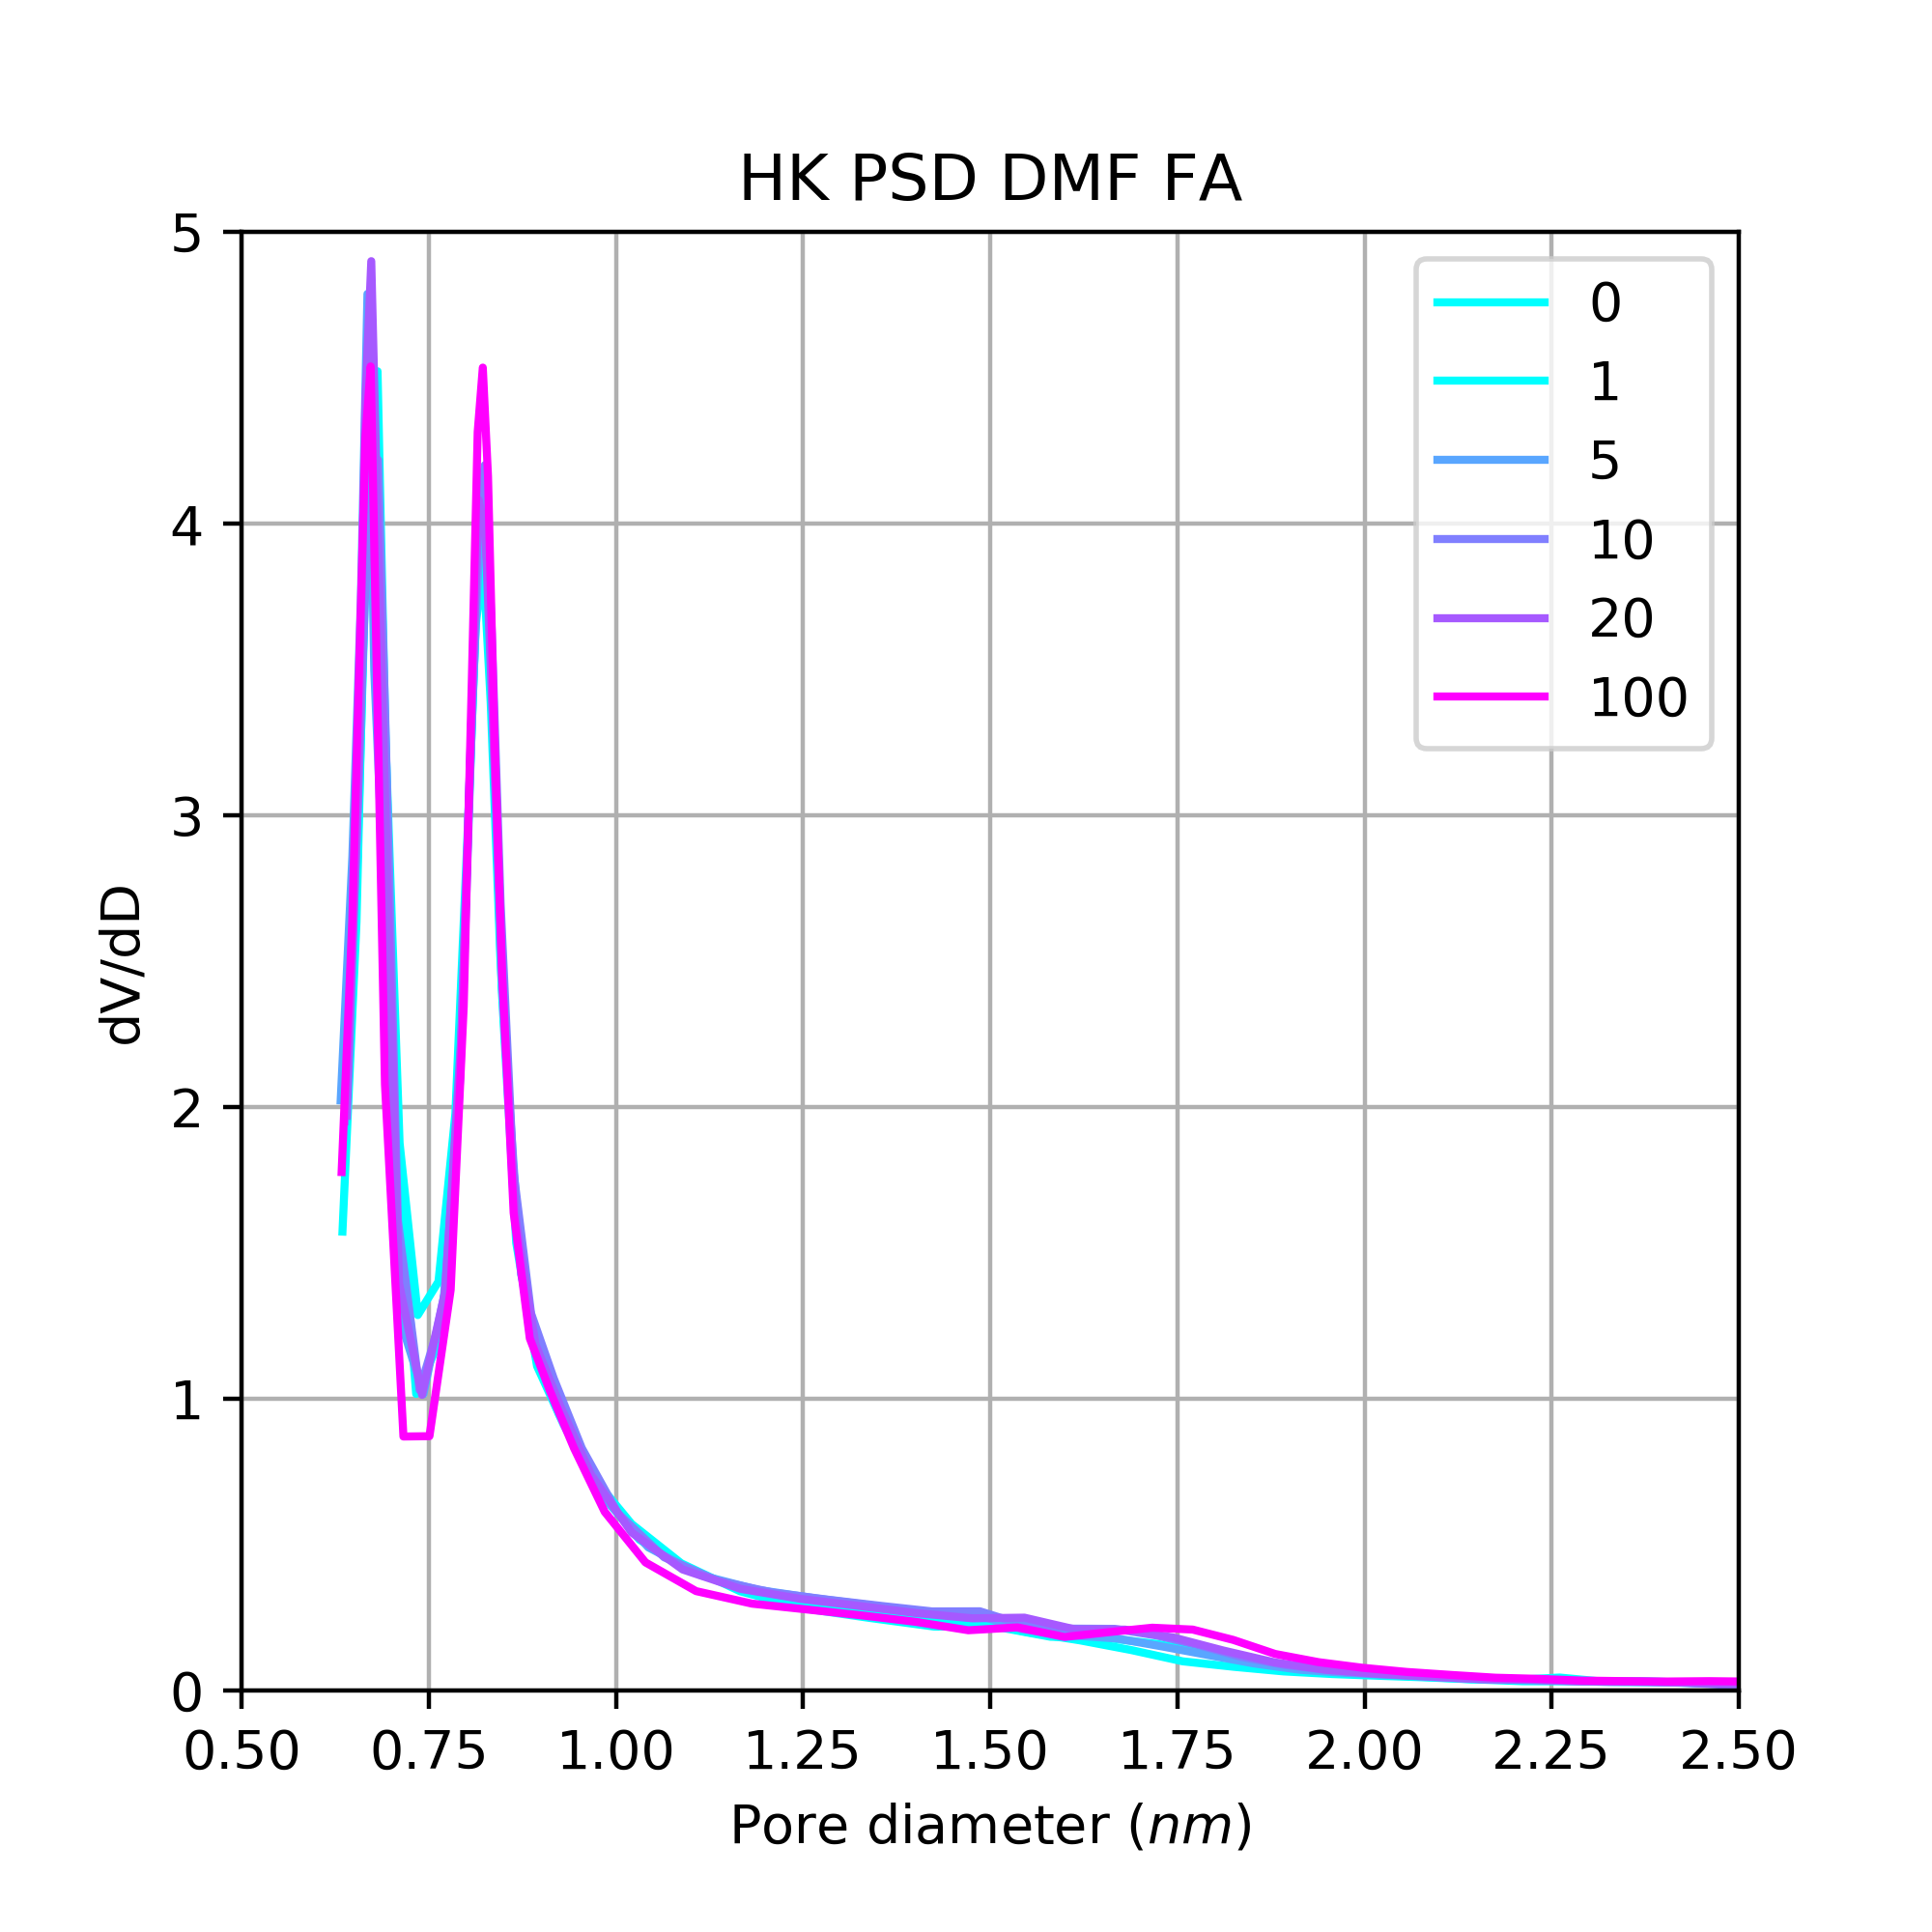
\includegraphics[width=\textwidth]{n2phys/dmf-fa-psd-hk}%
        \label{appx:def:fgr:psd-dmf-fa-hk}
    \end{subfigure}%
    \begin{subfigure}{0.25\linewidth}
        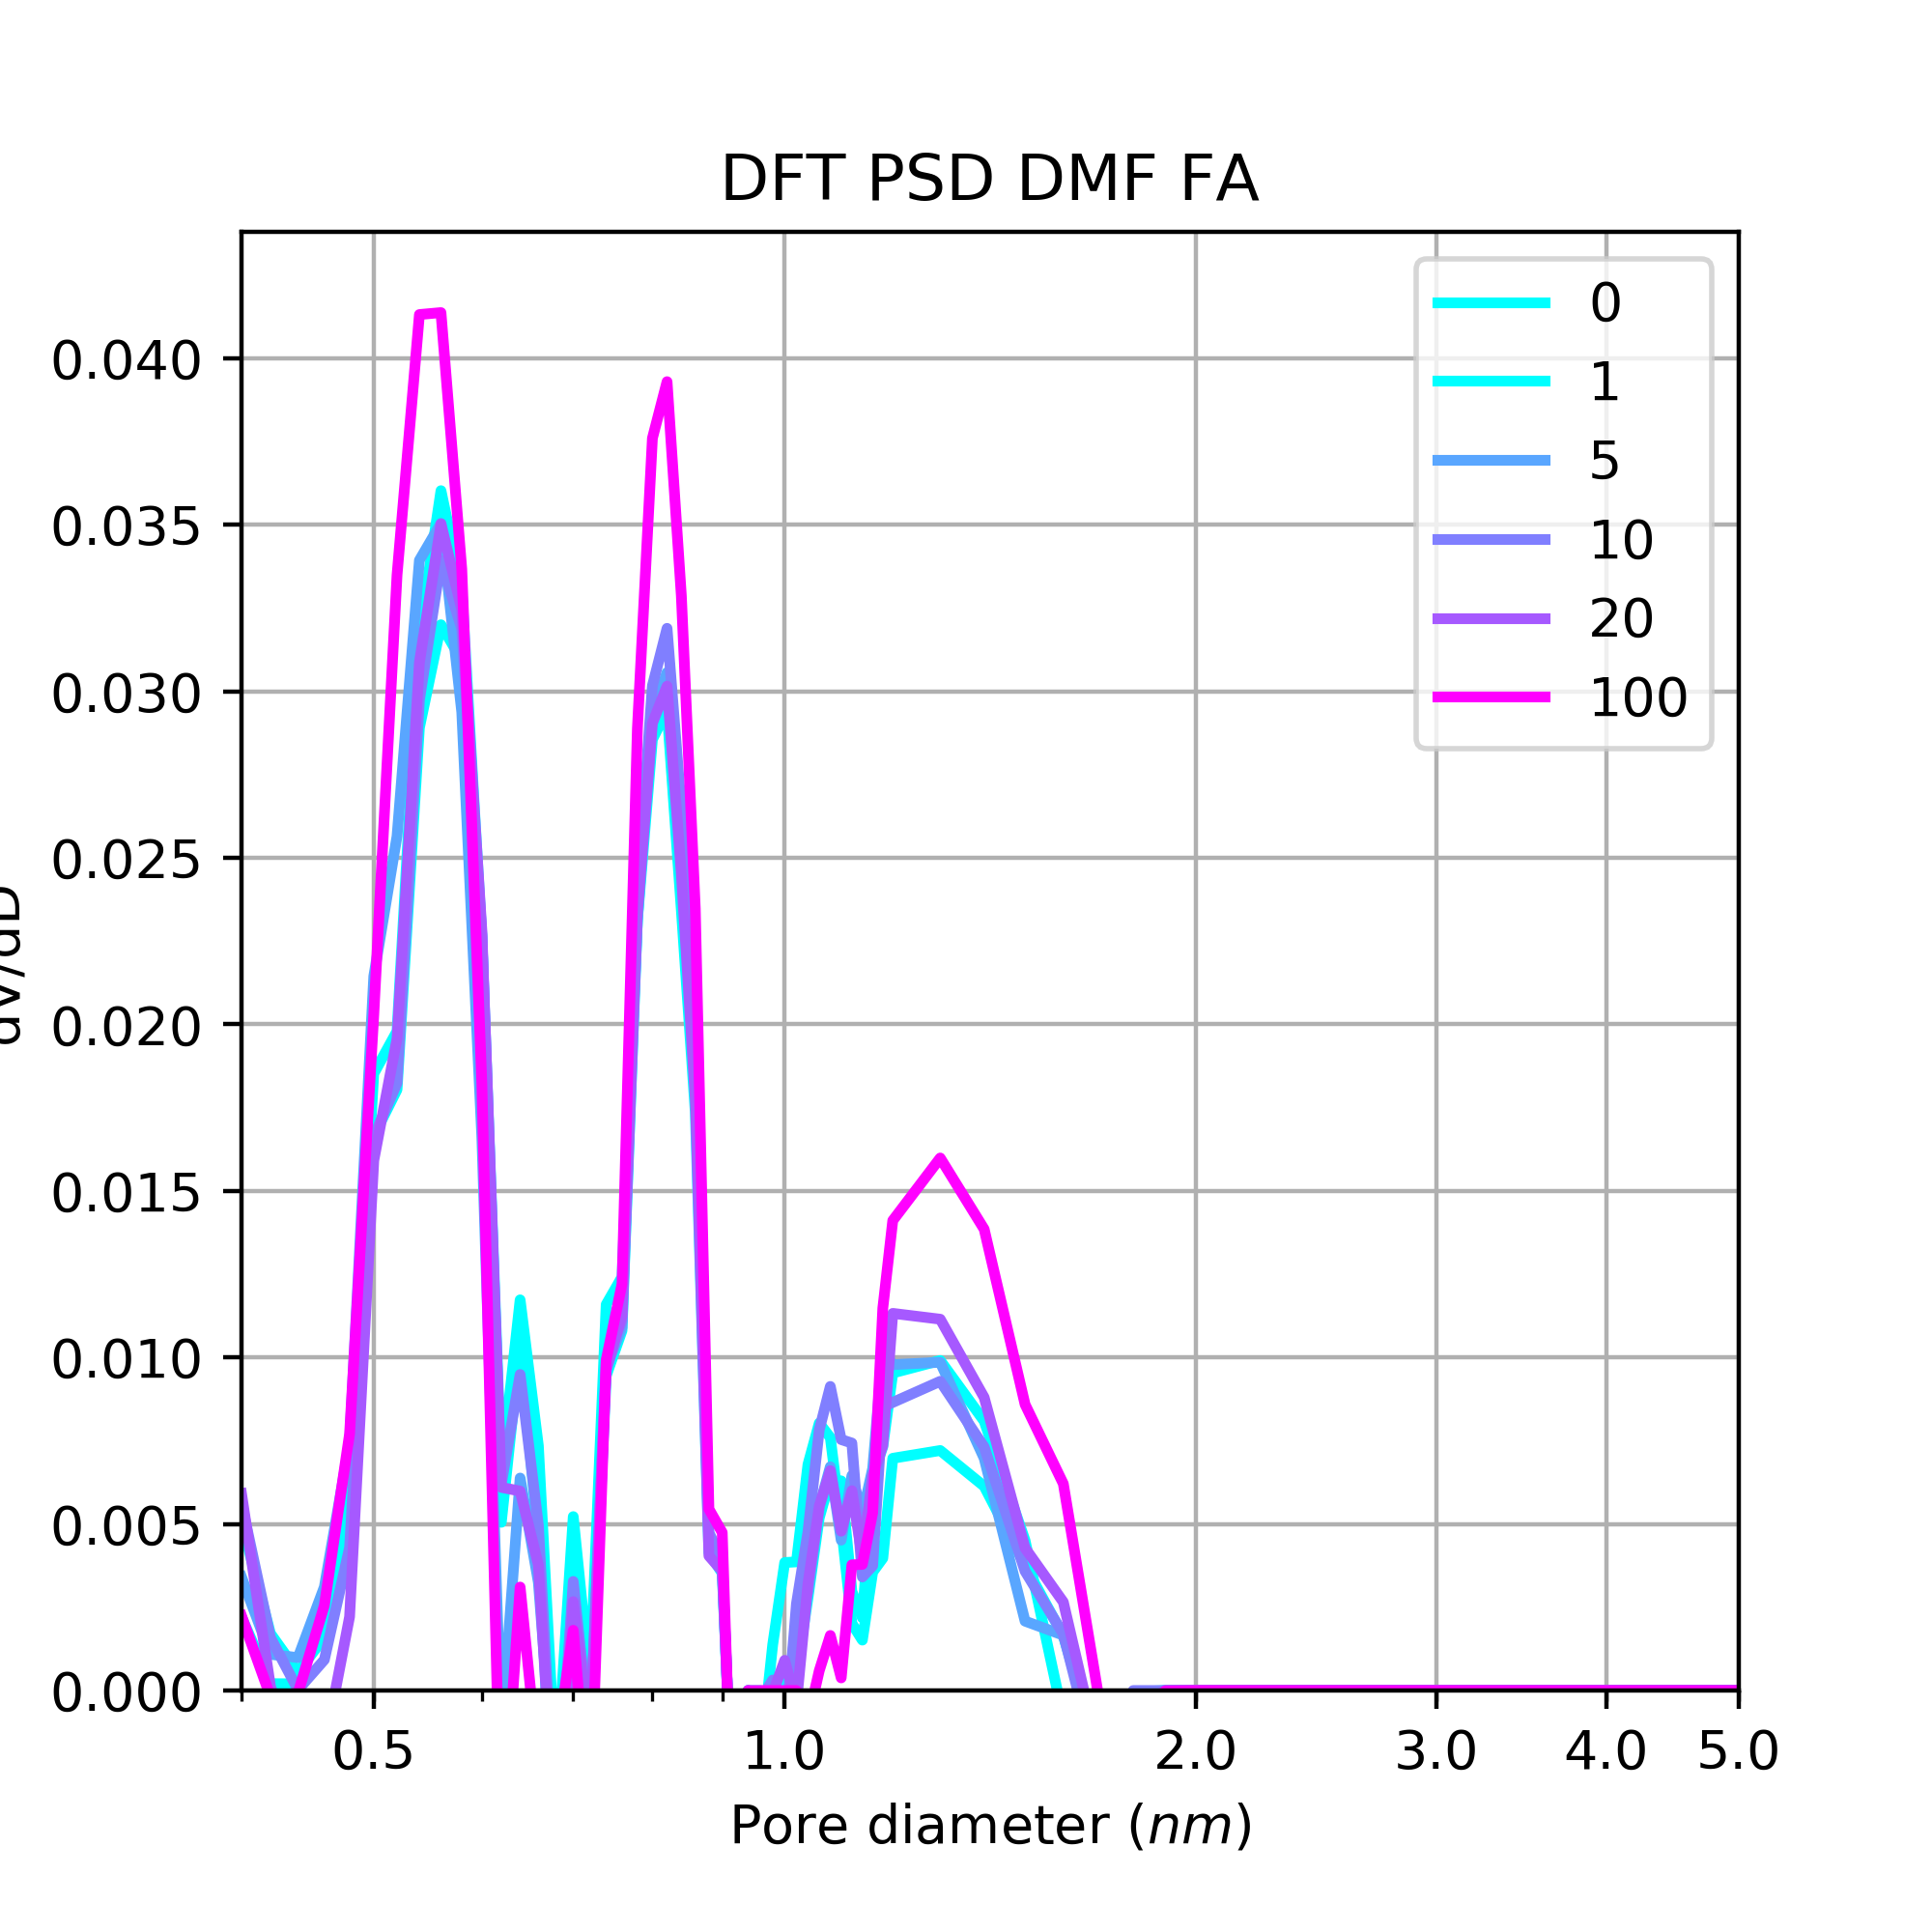
\includegraphics[width=\textwidth]{n2phys/dmf-fa-psd-dft}%
        \label{appx:def:fgr:psd-dmf-fa-dft}
    \end{subfigure}%
    \begin{subfigure}{0.25\linewidth}
        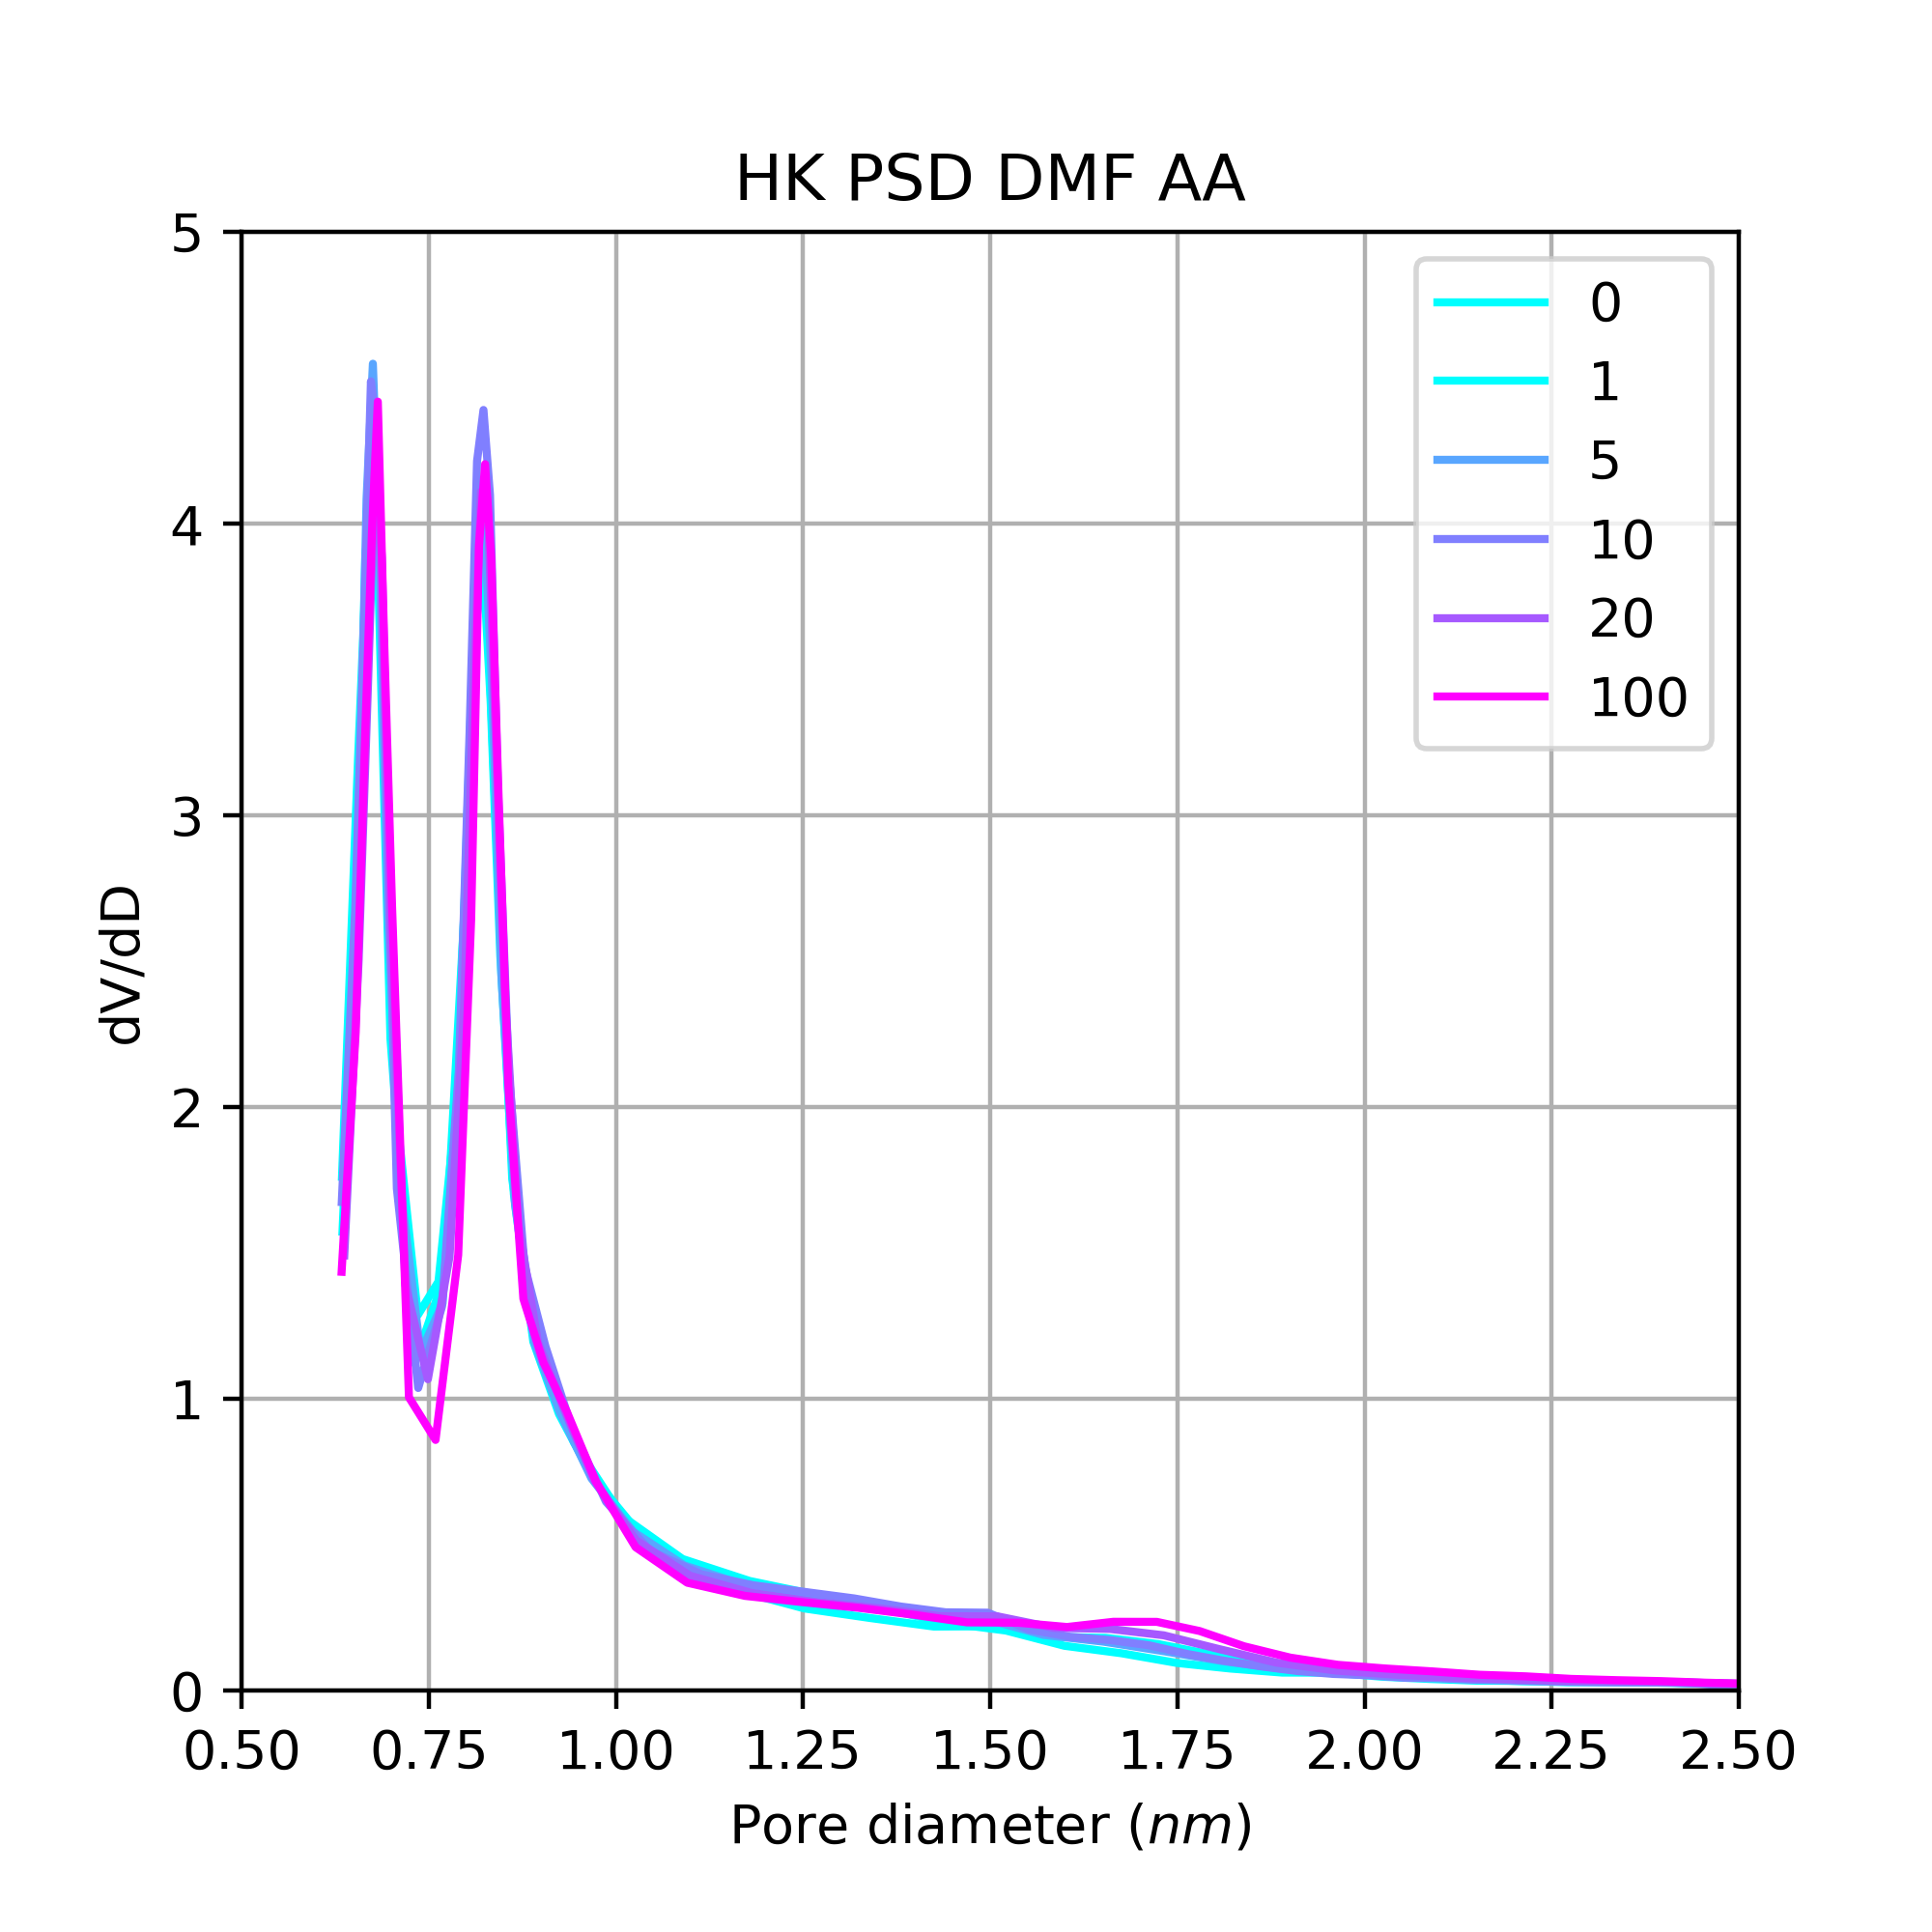
\includegraphics[width=\textwidth]{n2phys/dmf-aa-psd-hk}%
        \label{appx:def:fgr:psd-dmf-aa-hk}
    \end{subfigure}%
    \begin{subfigure}{0.25\linewidth}
        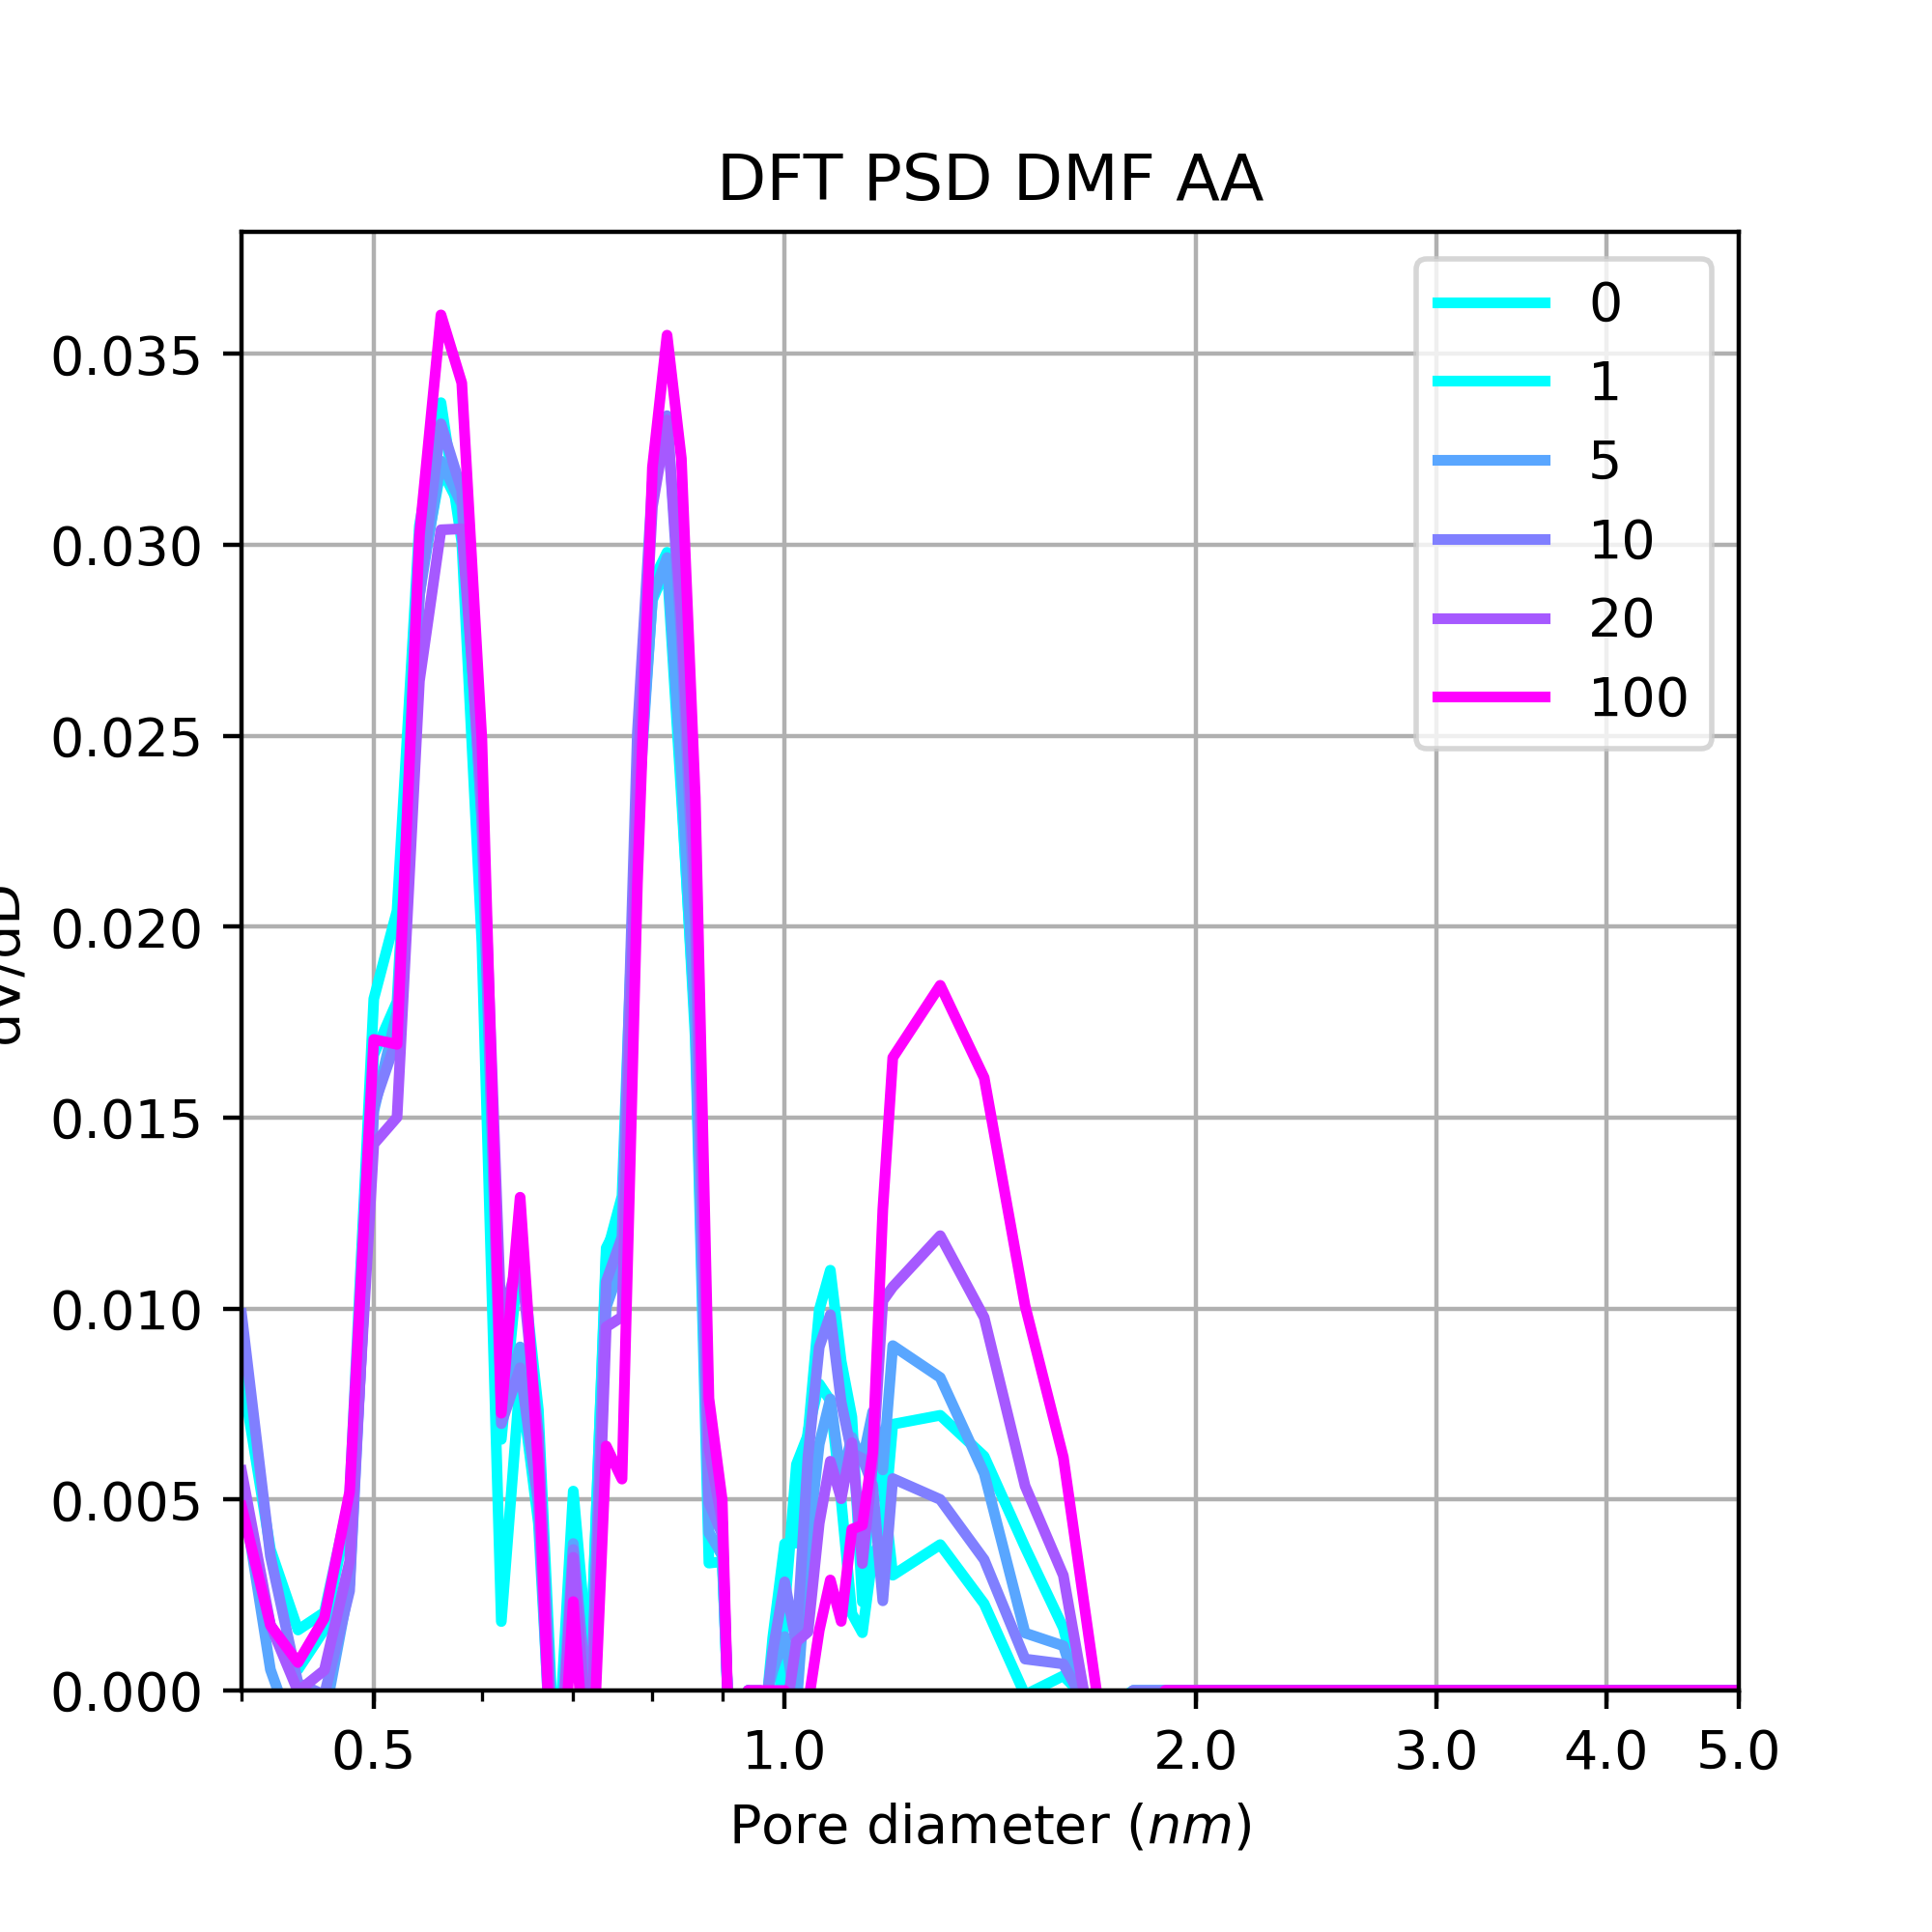
\includegraphics[width=\textwidth]{n2phys/dmf-aa-psd-dft}%
        \label{appx:def:fgr:psd-dmf-aa-dft}
    \end{subfigure}%

    \begin{subfigure}{0.25\linewidth}
        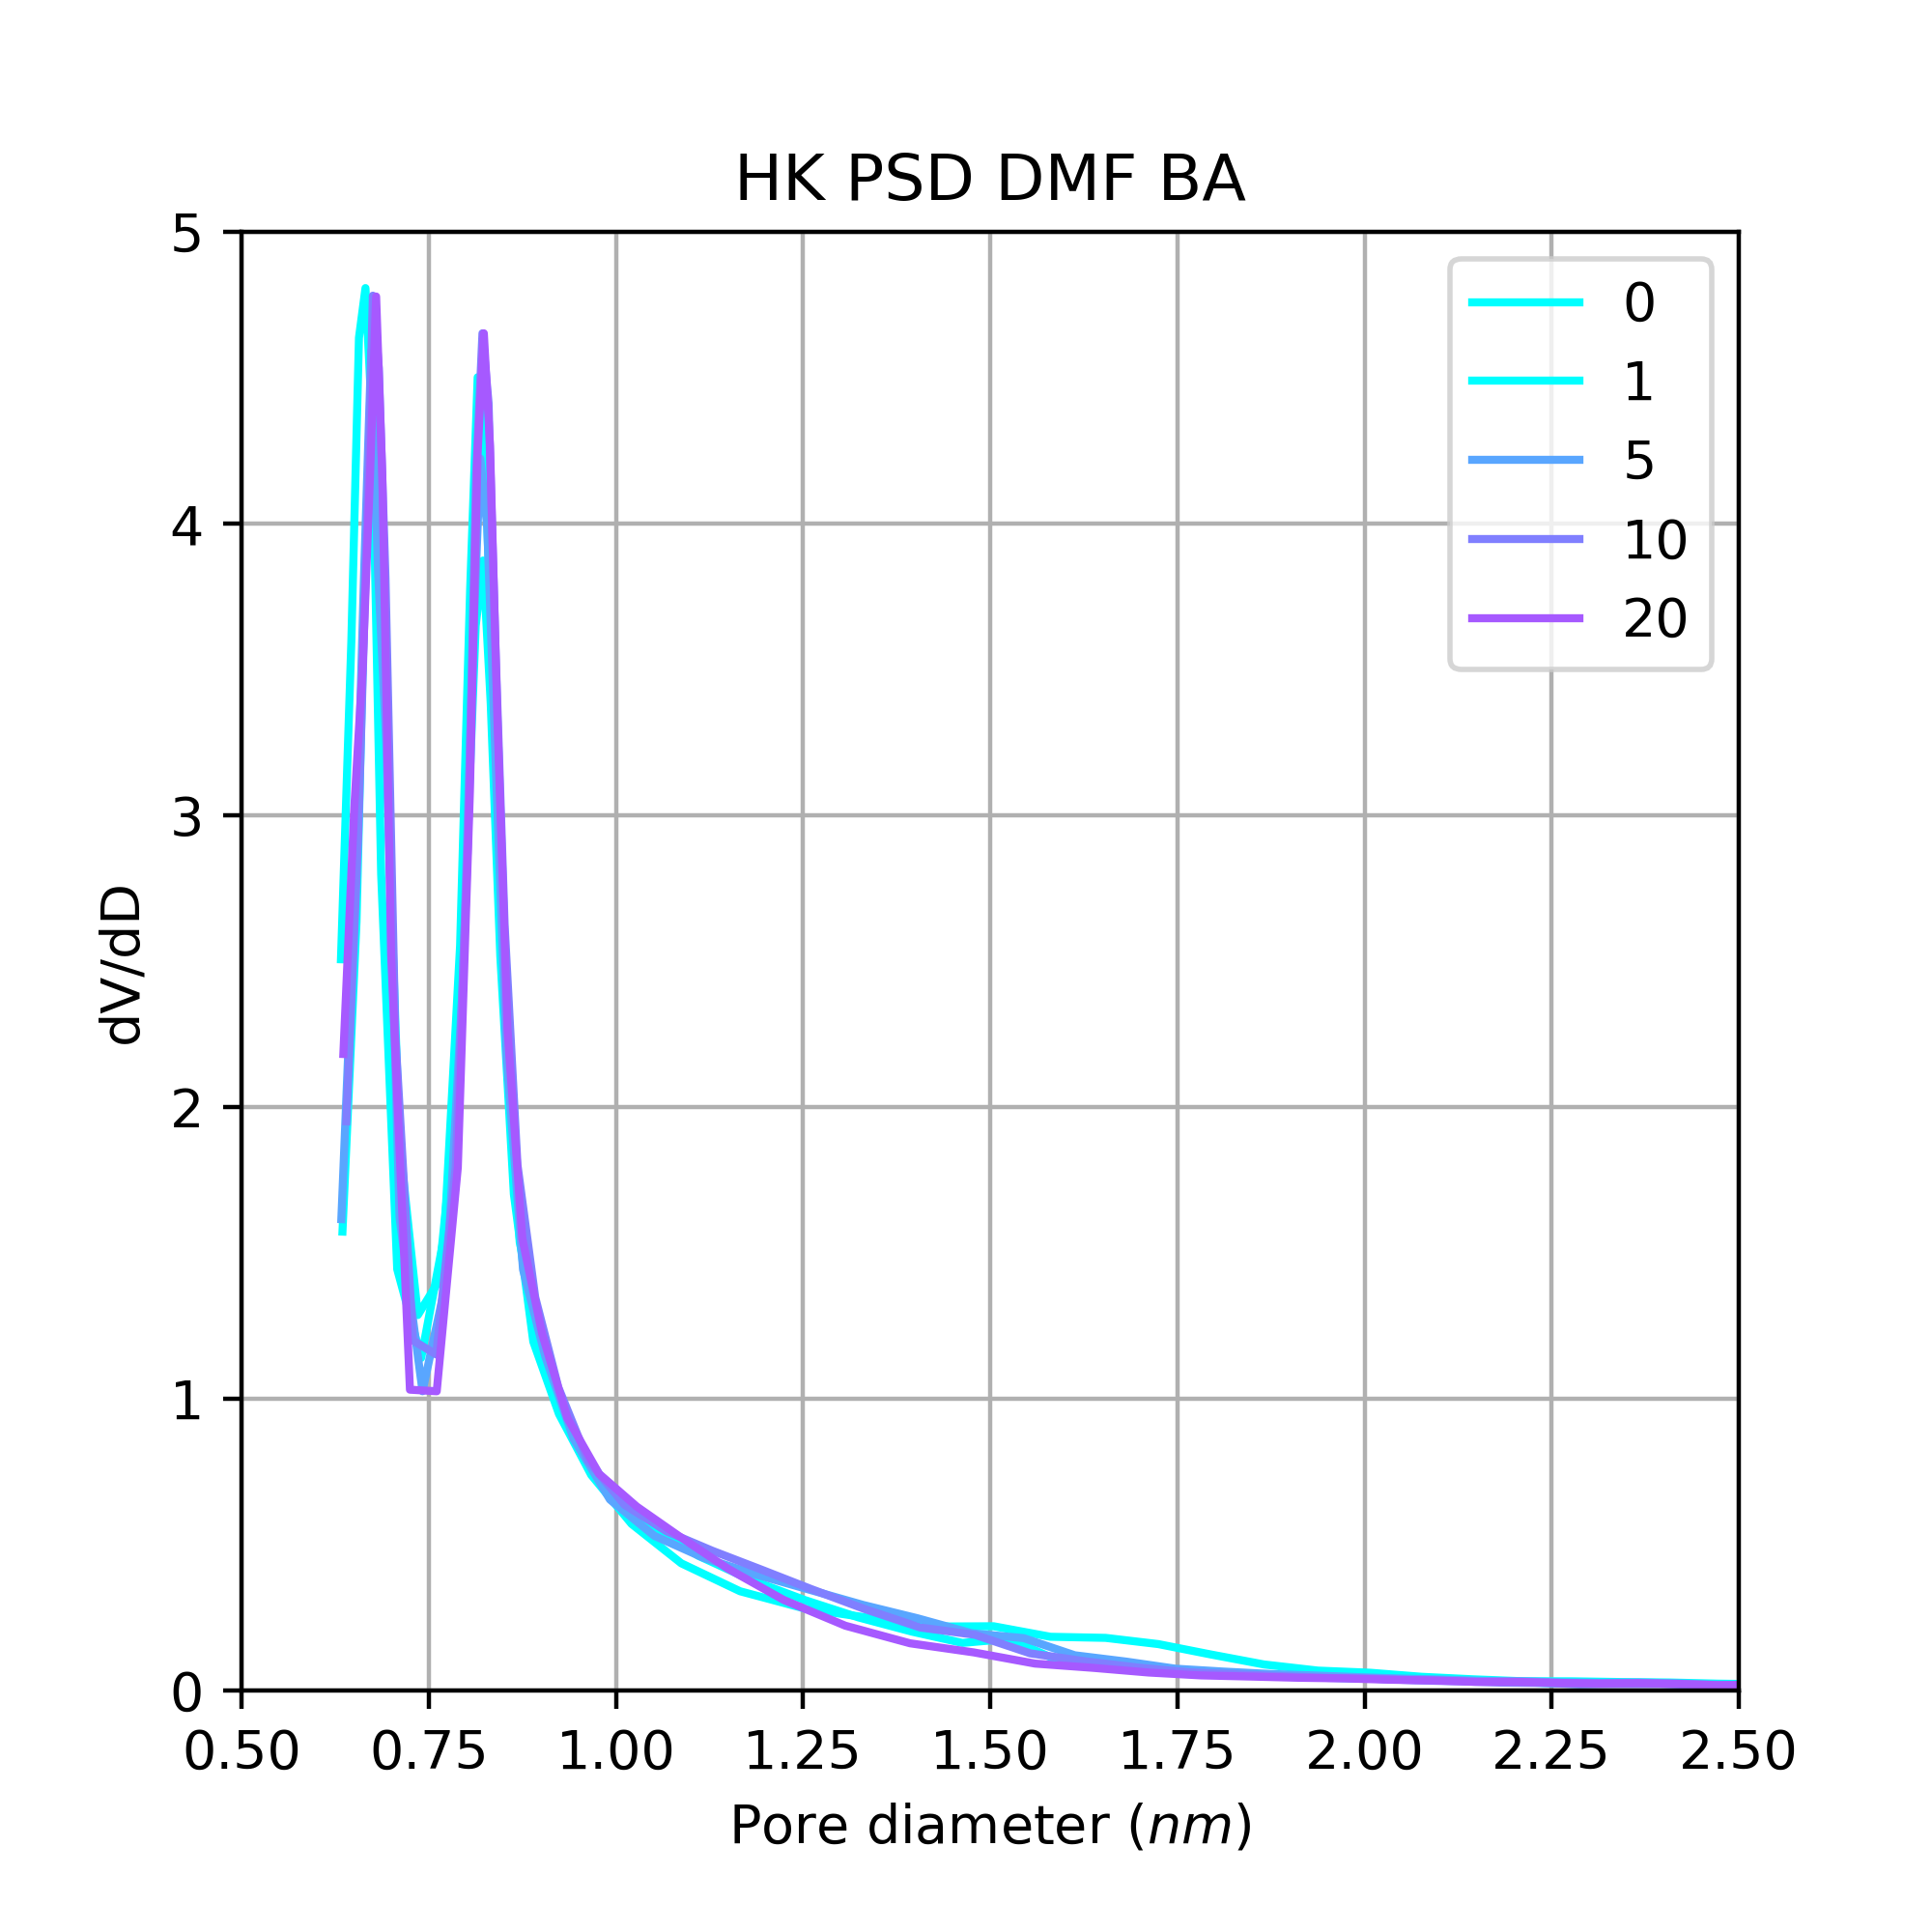
\includegraphics[width=\textwidth]{n2phys/dmf-ba-psd-hk}%
        \label{appx:def:fgr:psd-dmf-ba-hk}
    \end{subfigure}%
    \begin{subfigure}{0.25\linewidth}
        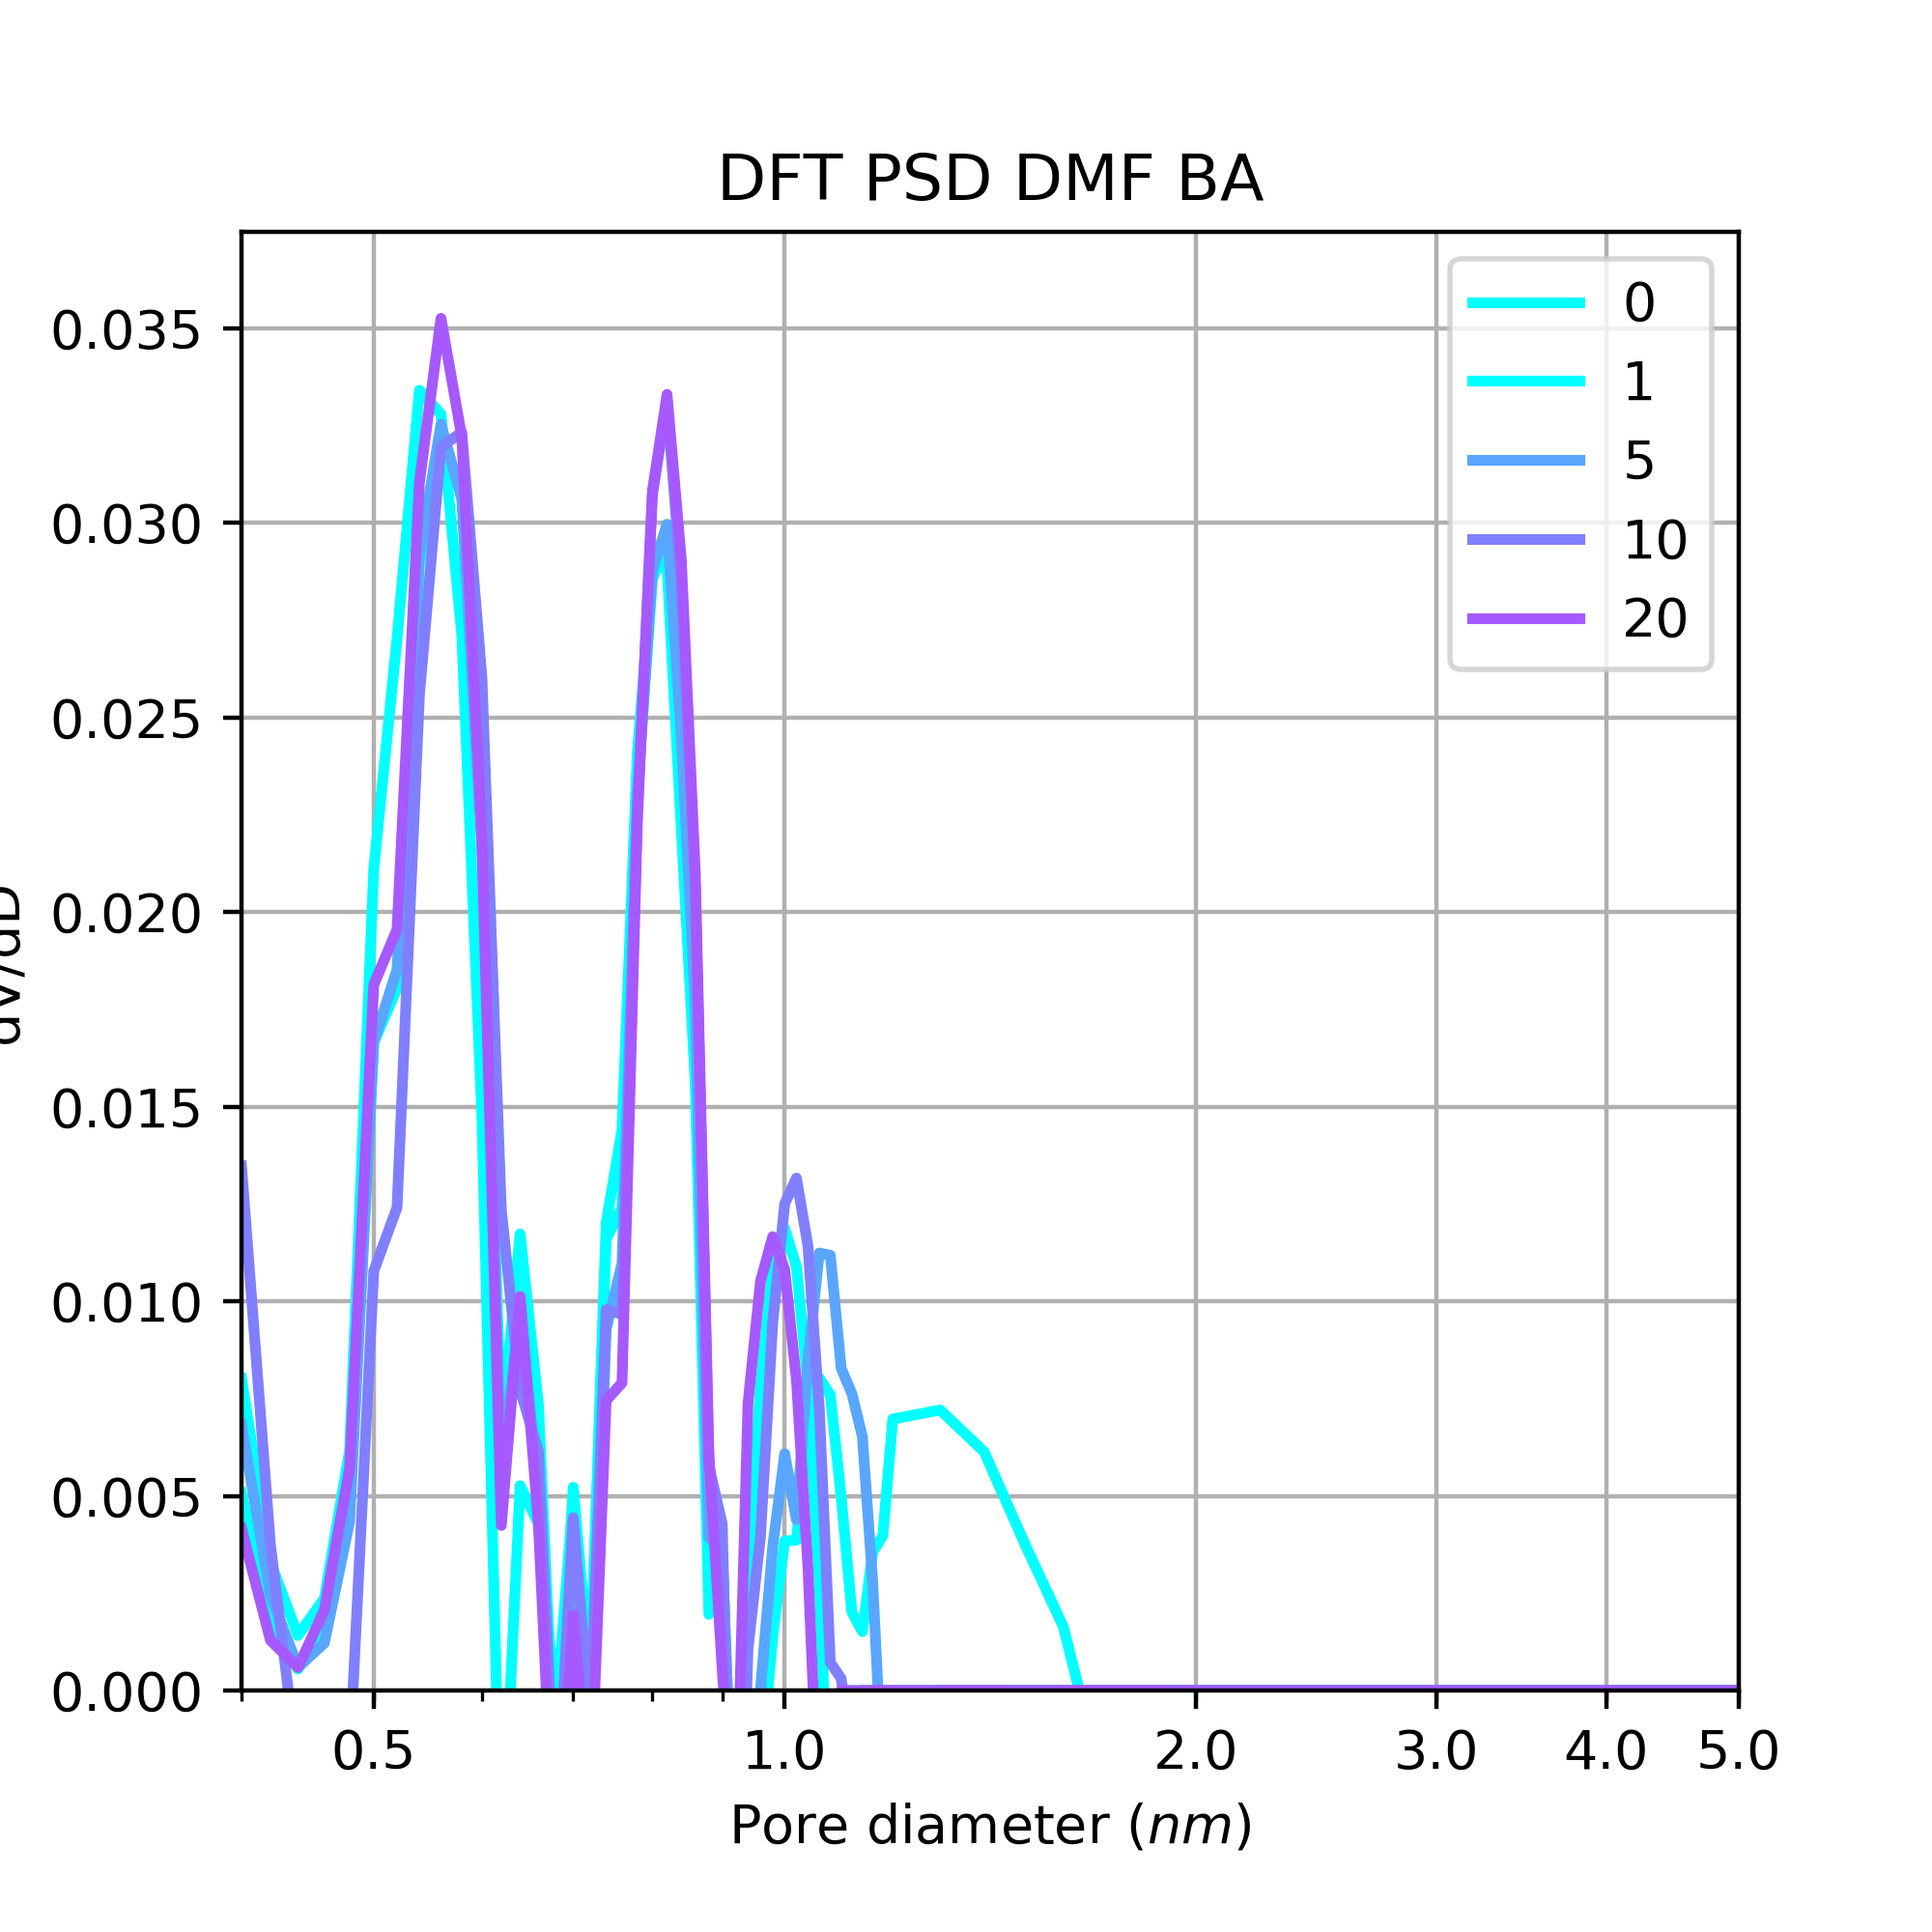
\includegraphics[width=\textwidth]{n2phys/dmf-ba-psd-dft}%
        \label{appx:def:fgr:psd-dmf-ba-dft}
    \end{subfigure}%

    \begin{subfigure}{0.25\linewidth}
        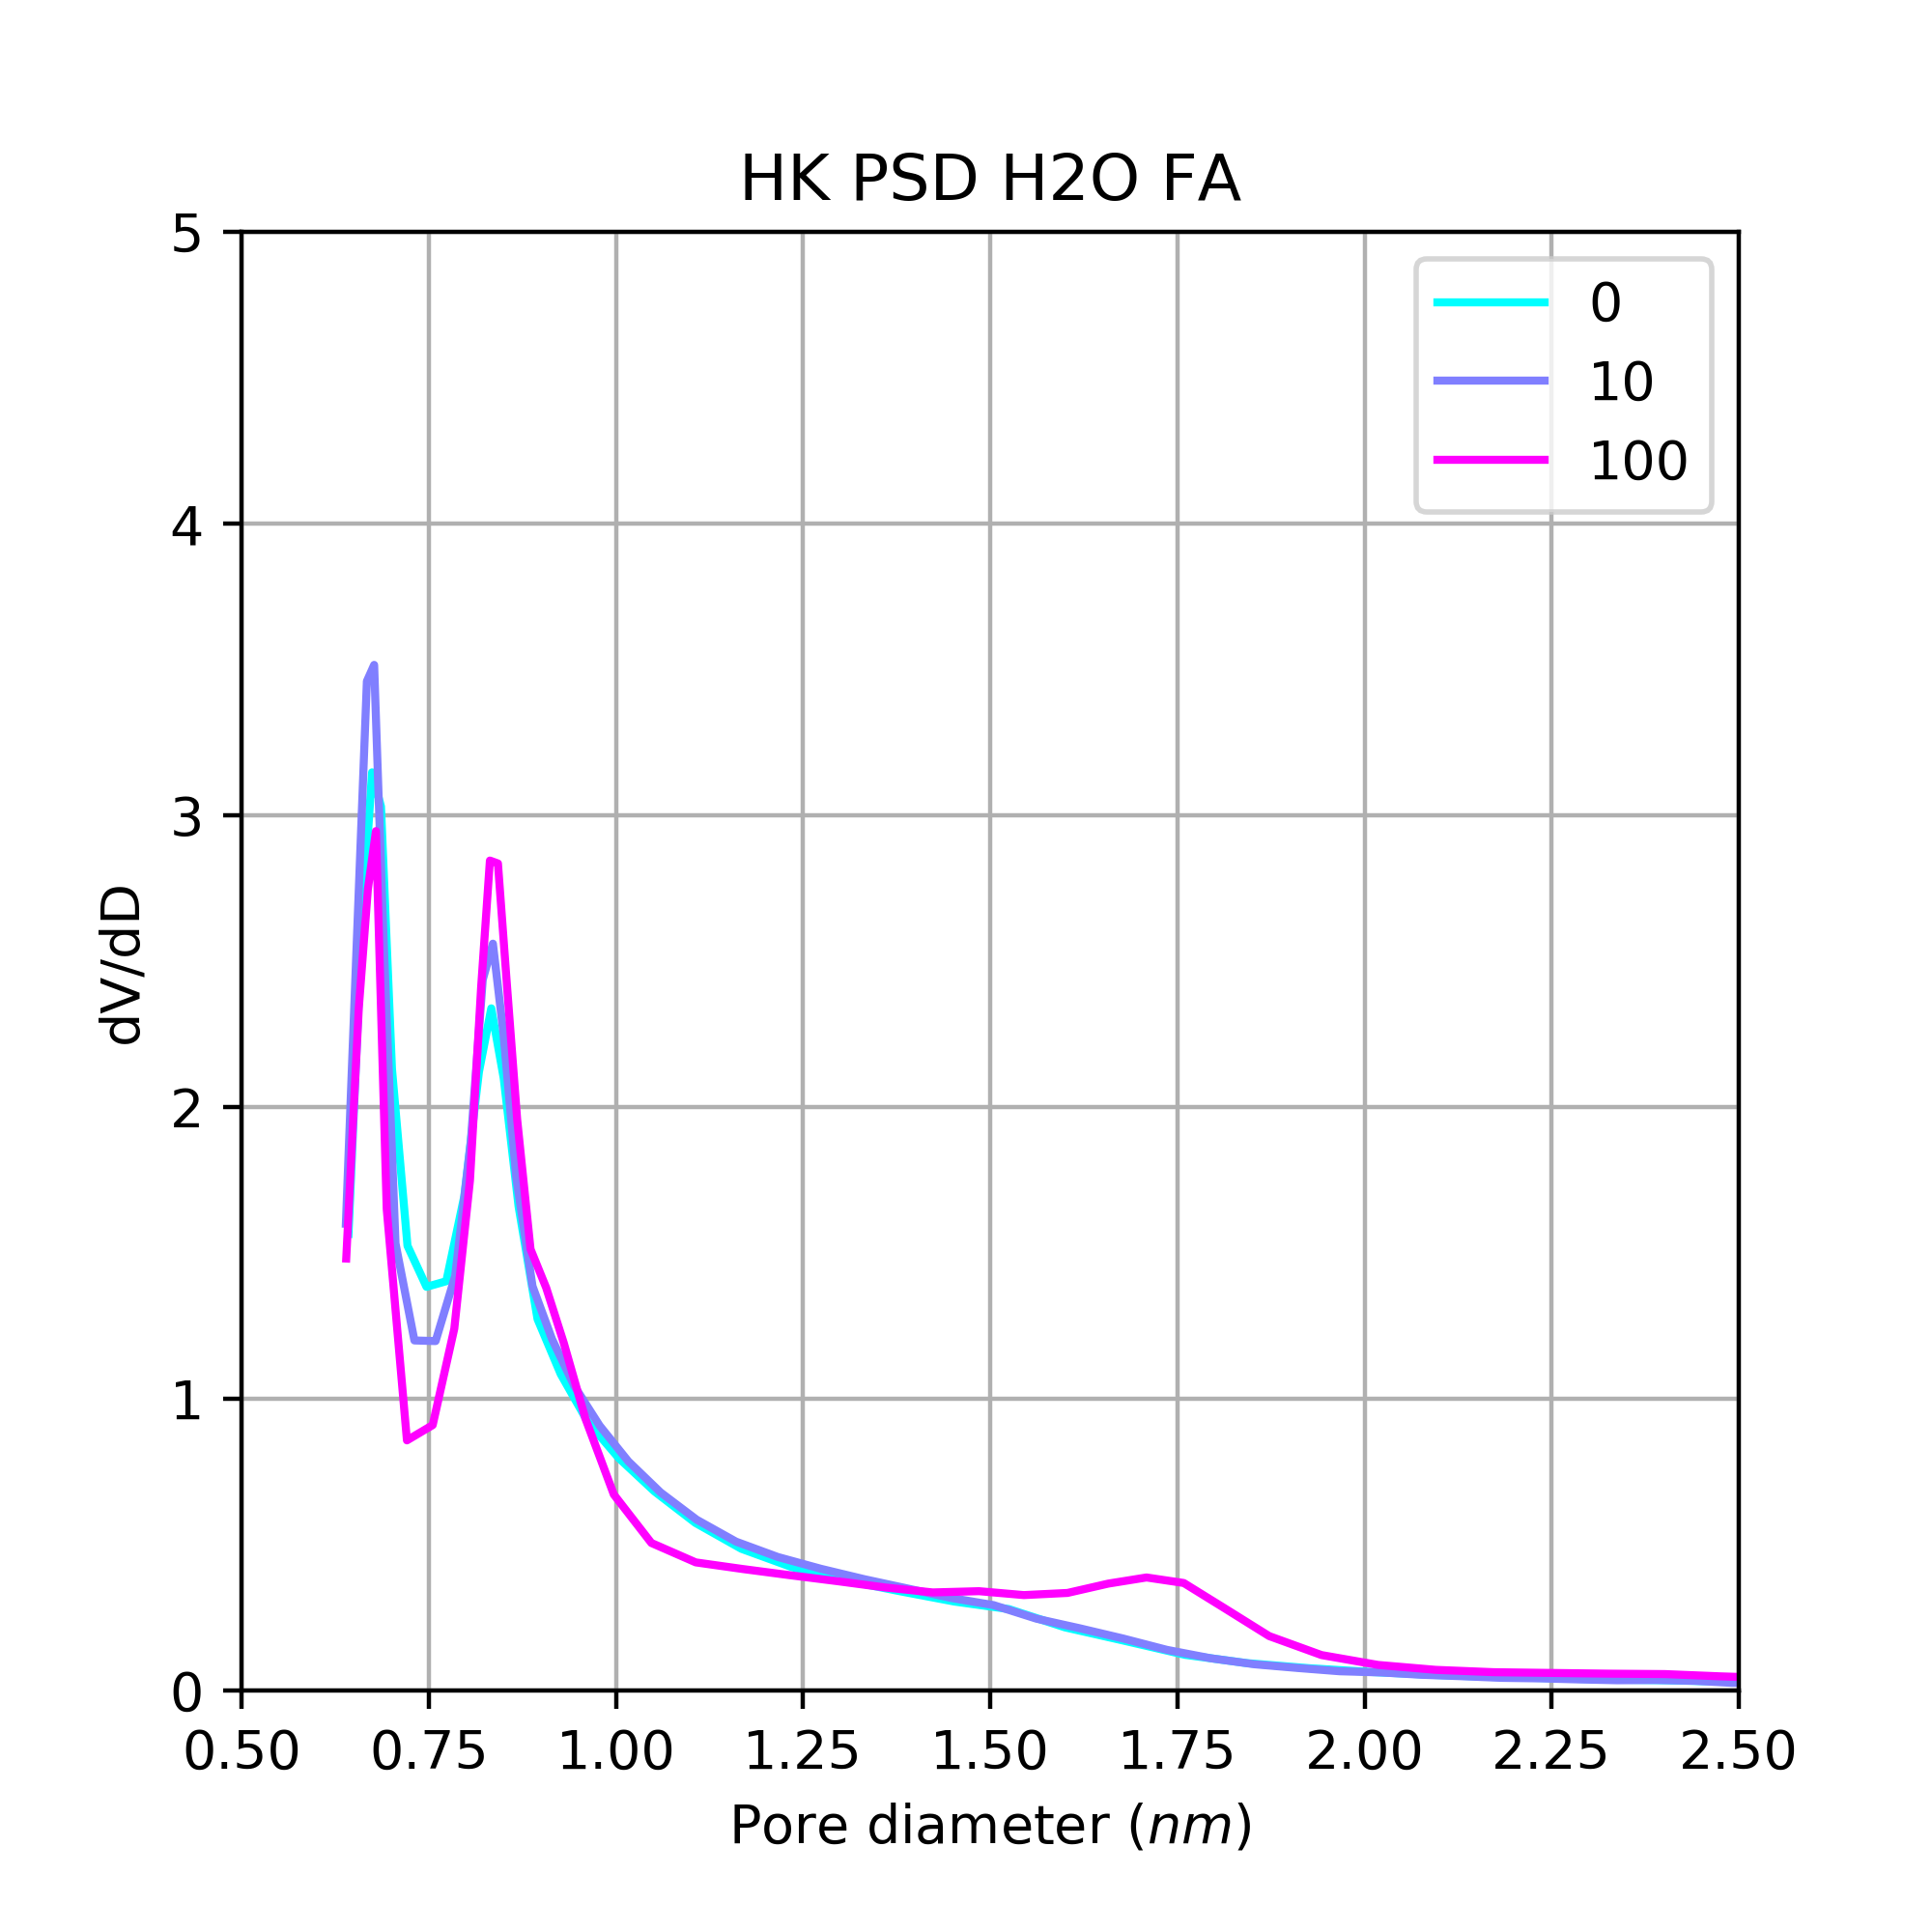
\includegraphics[width=\textwidth]{n2phys/h2o-fa-psd-hk}%
        \label{appx:def:fgr:psd-h2o-fa-hk}
    \end{subfigure}%
    \begin{subfigure}{0.25\linewidth}
        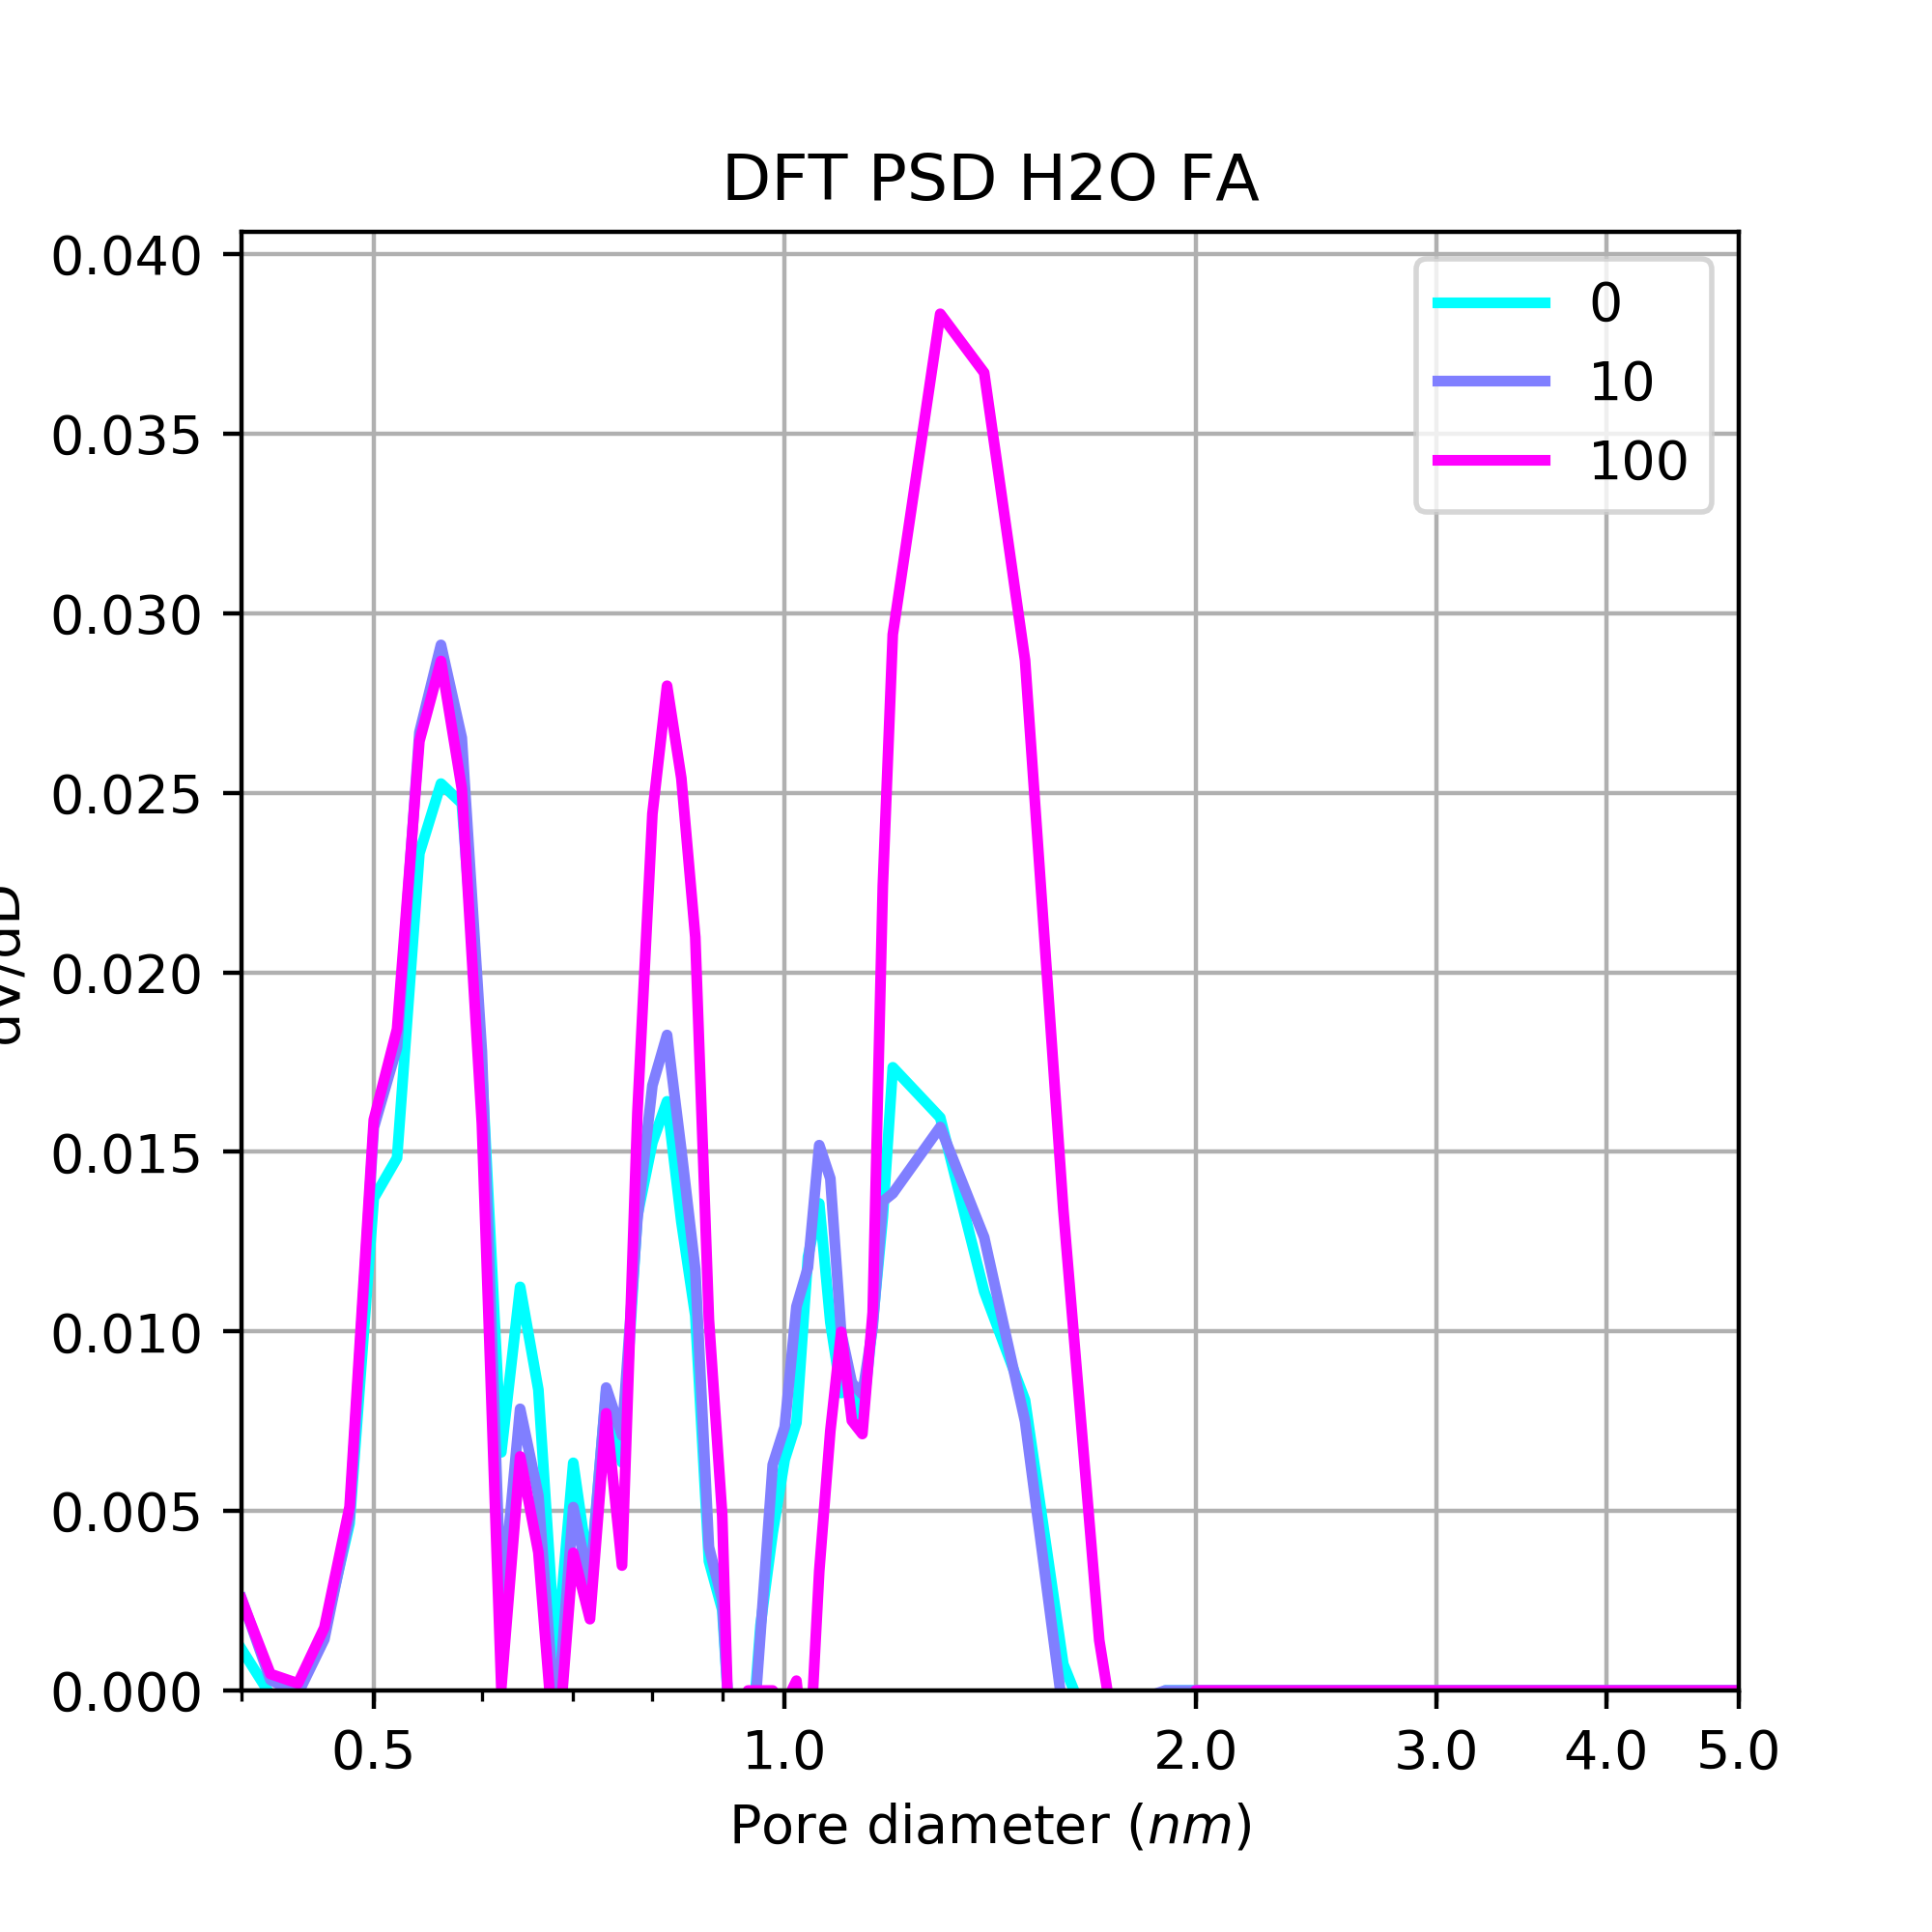
\includegraphics[width=\textwidth]{n2phys/h2o-fa-psd-dft}%
        \label{appx:def:fgr:psd-h2o-fa-dft}
    \end{subfigure}%
    \begin{subfigure}{0.25\linewidth}
        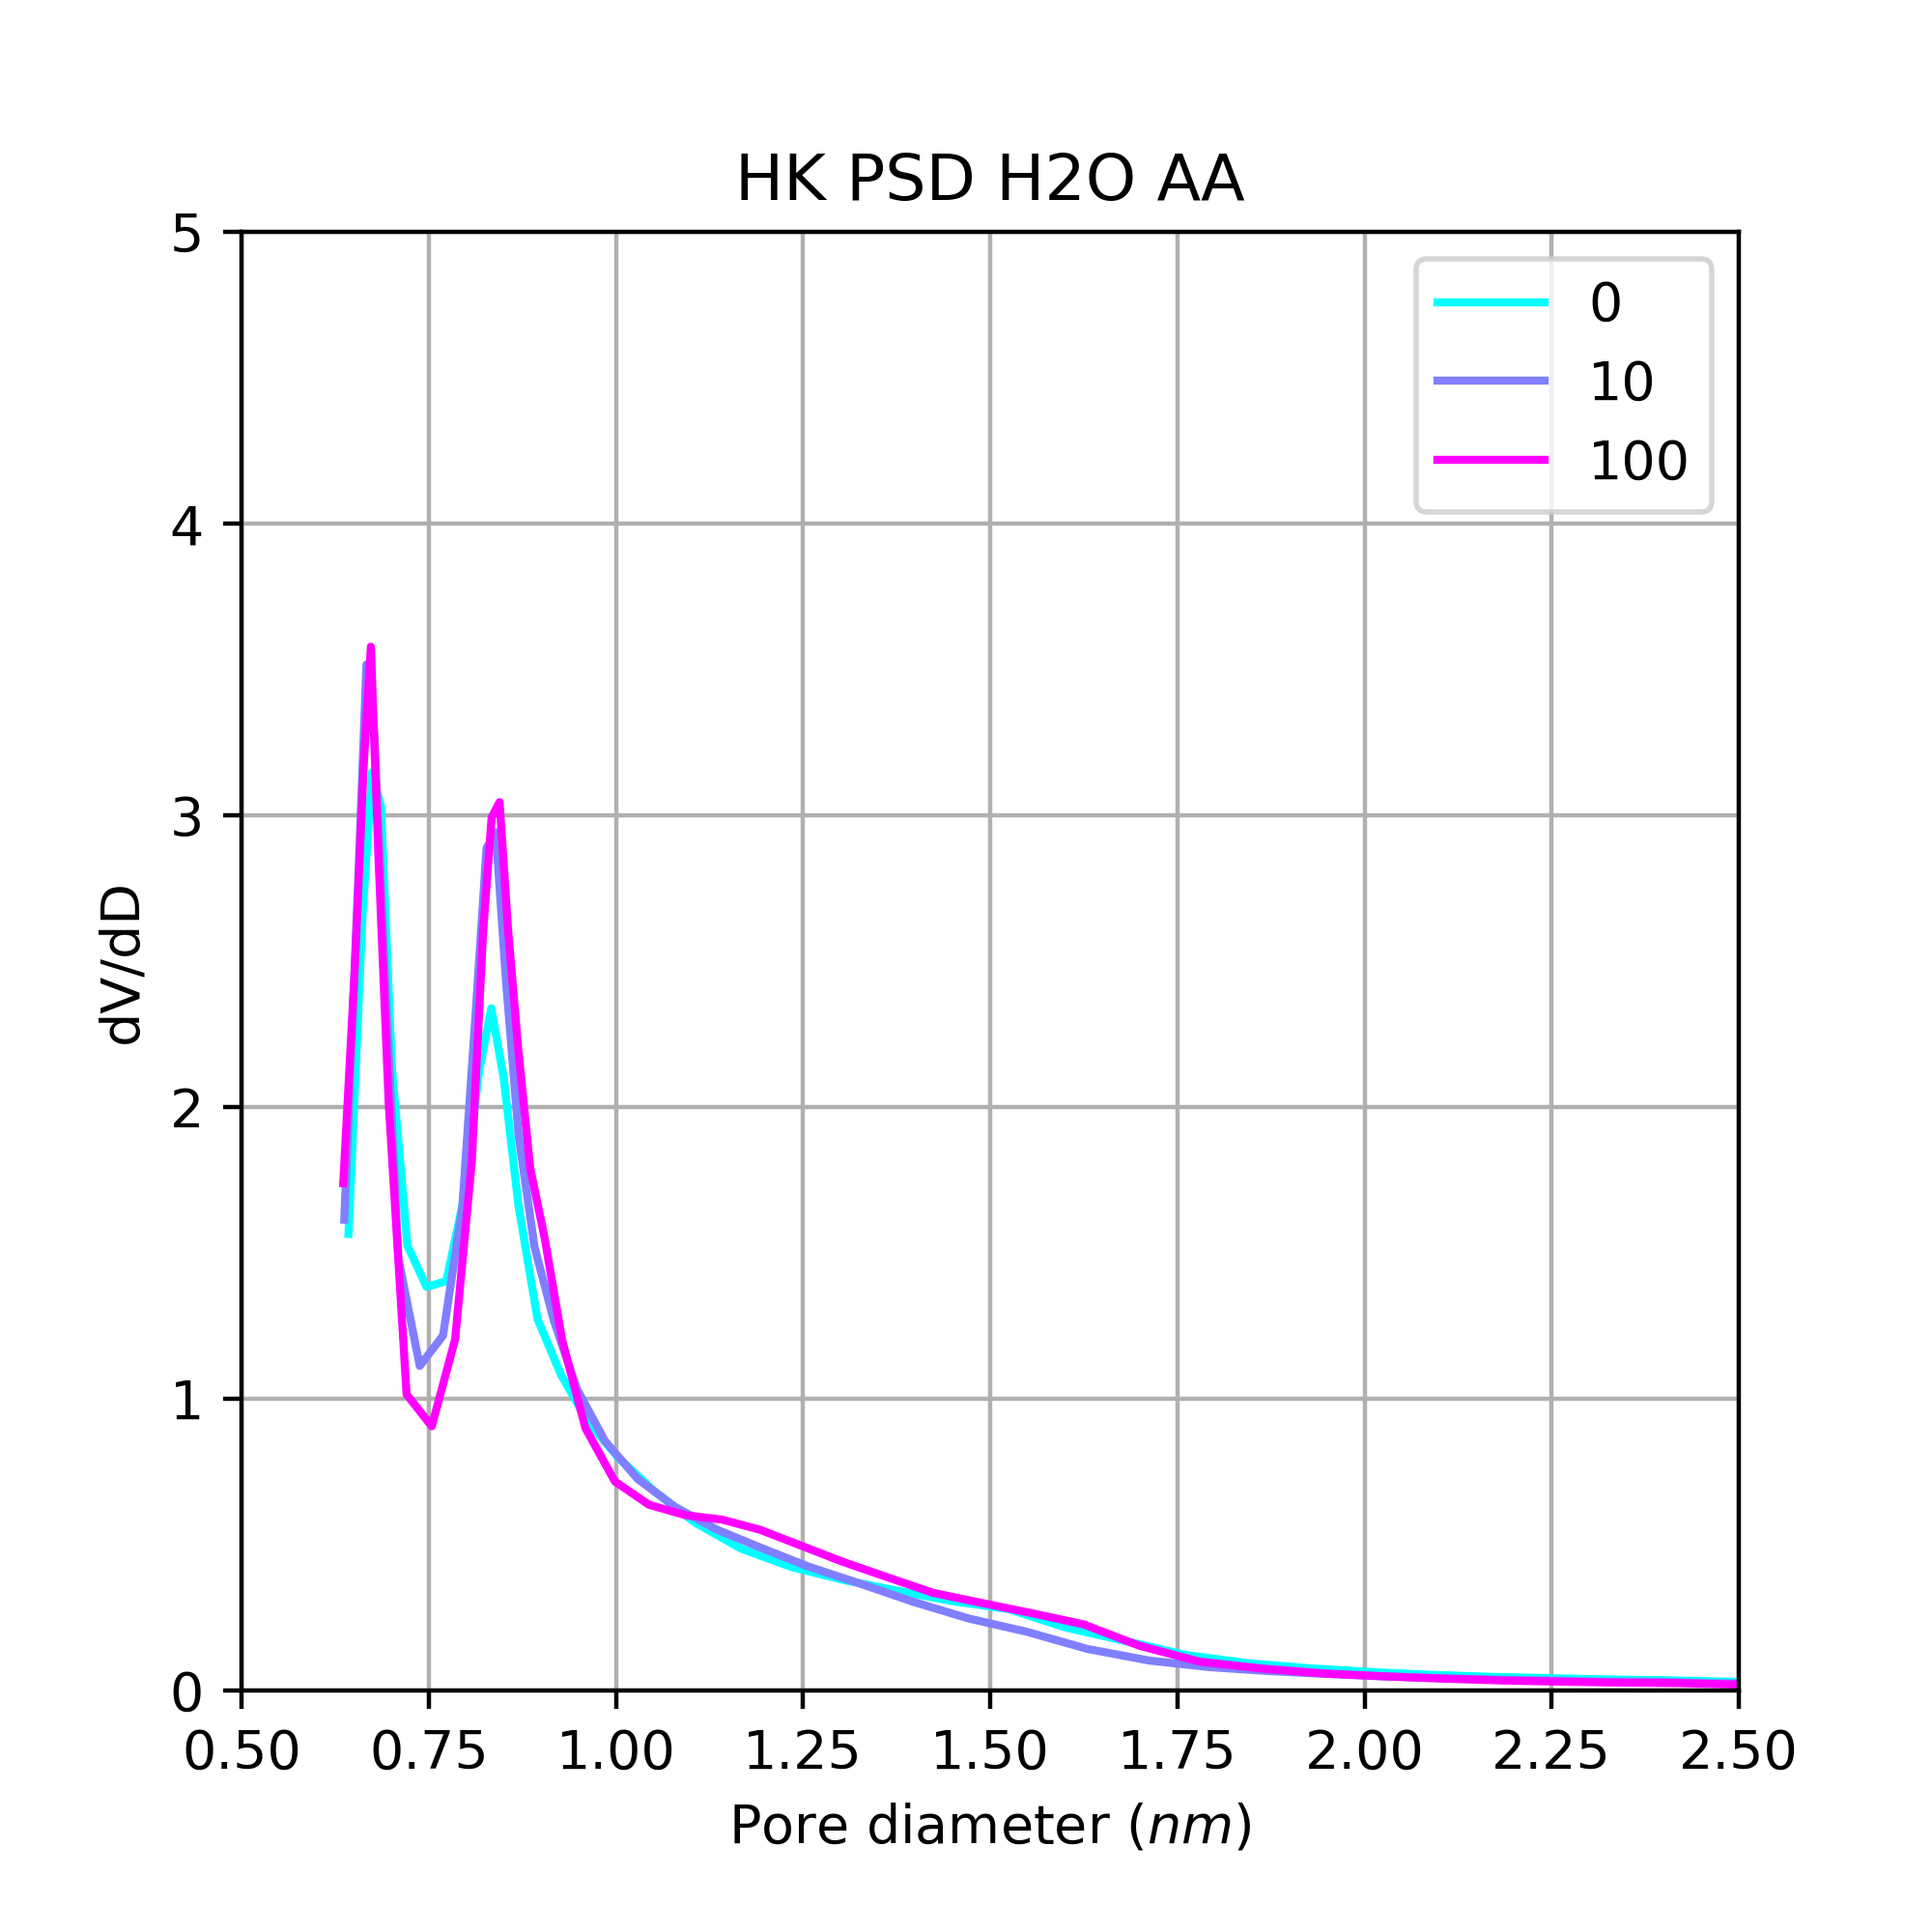
\includegraphics[width=\textwidth]{n2phys/h2o-aa-psd-hk}%
        \label{appx:def:fgr:psd-h2o-aa-hk}
    \end{subfigure}%
    \begin{subfigure}{0.25\linewidth}
        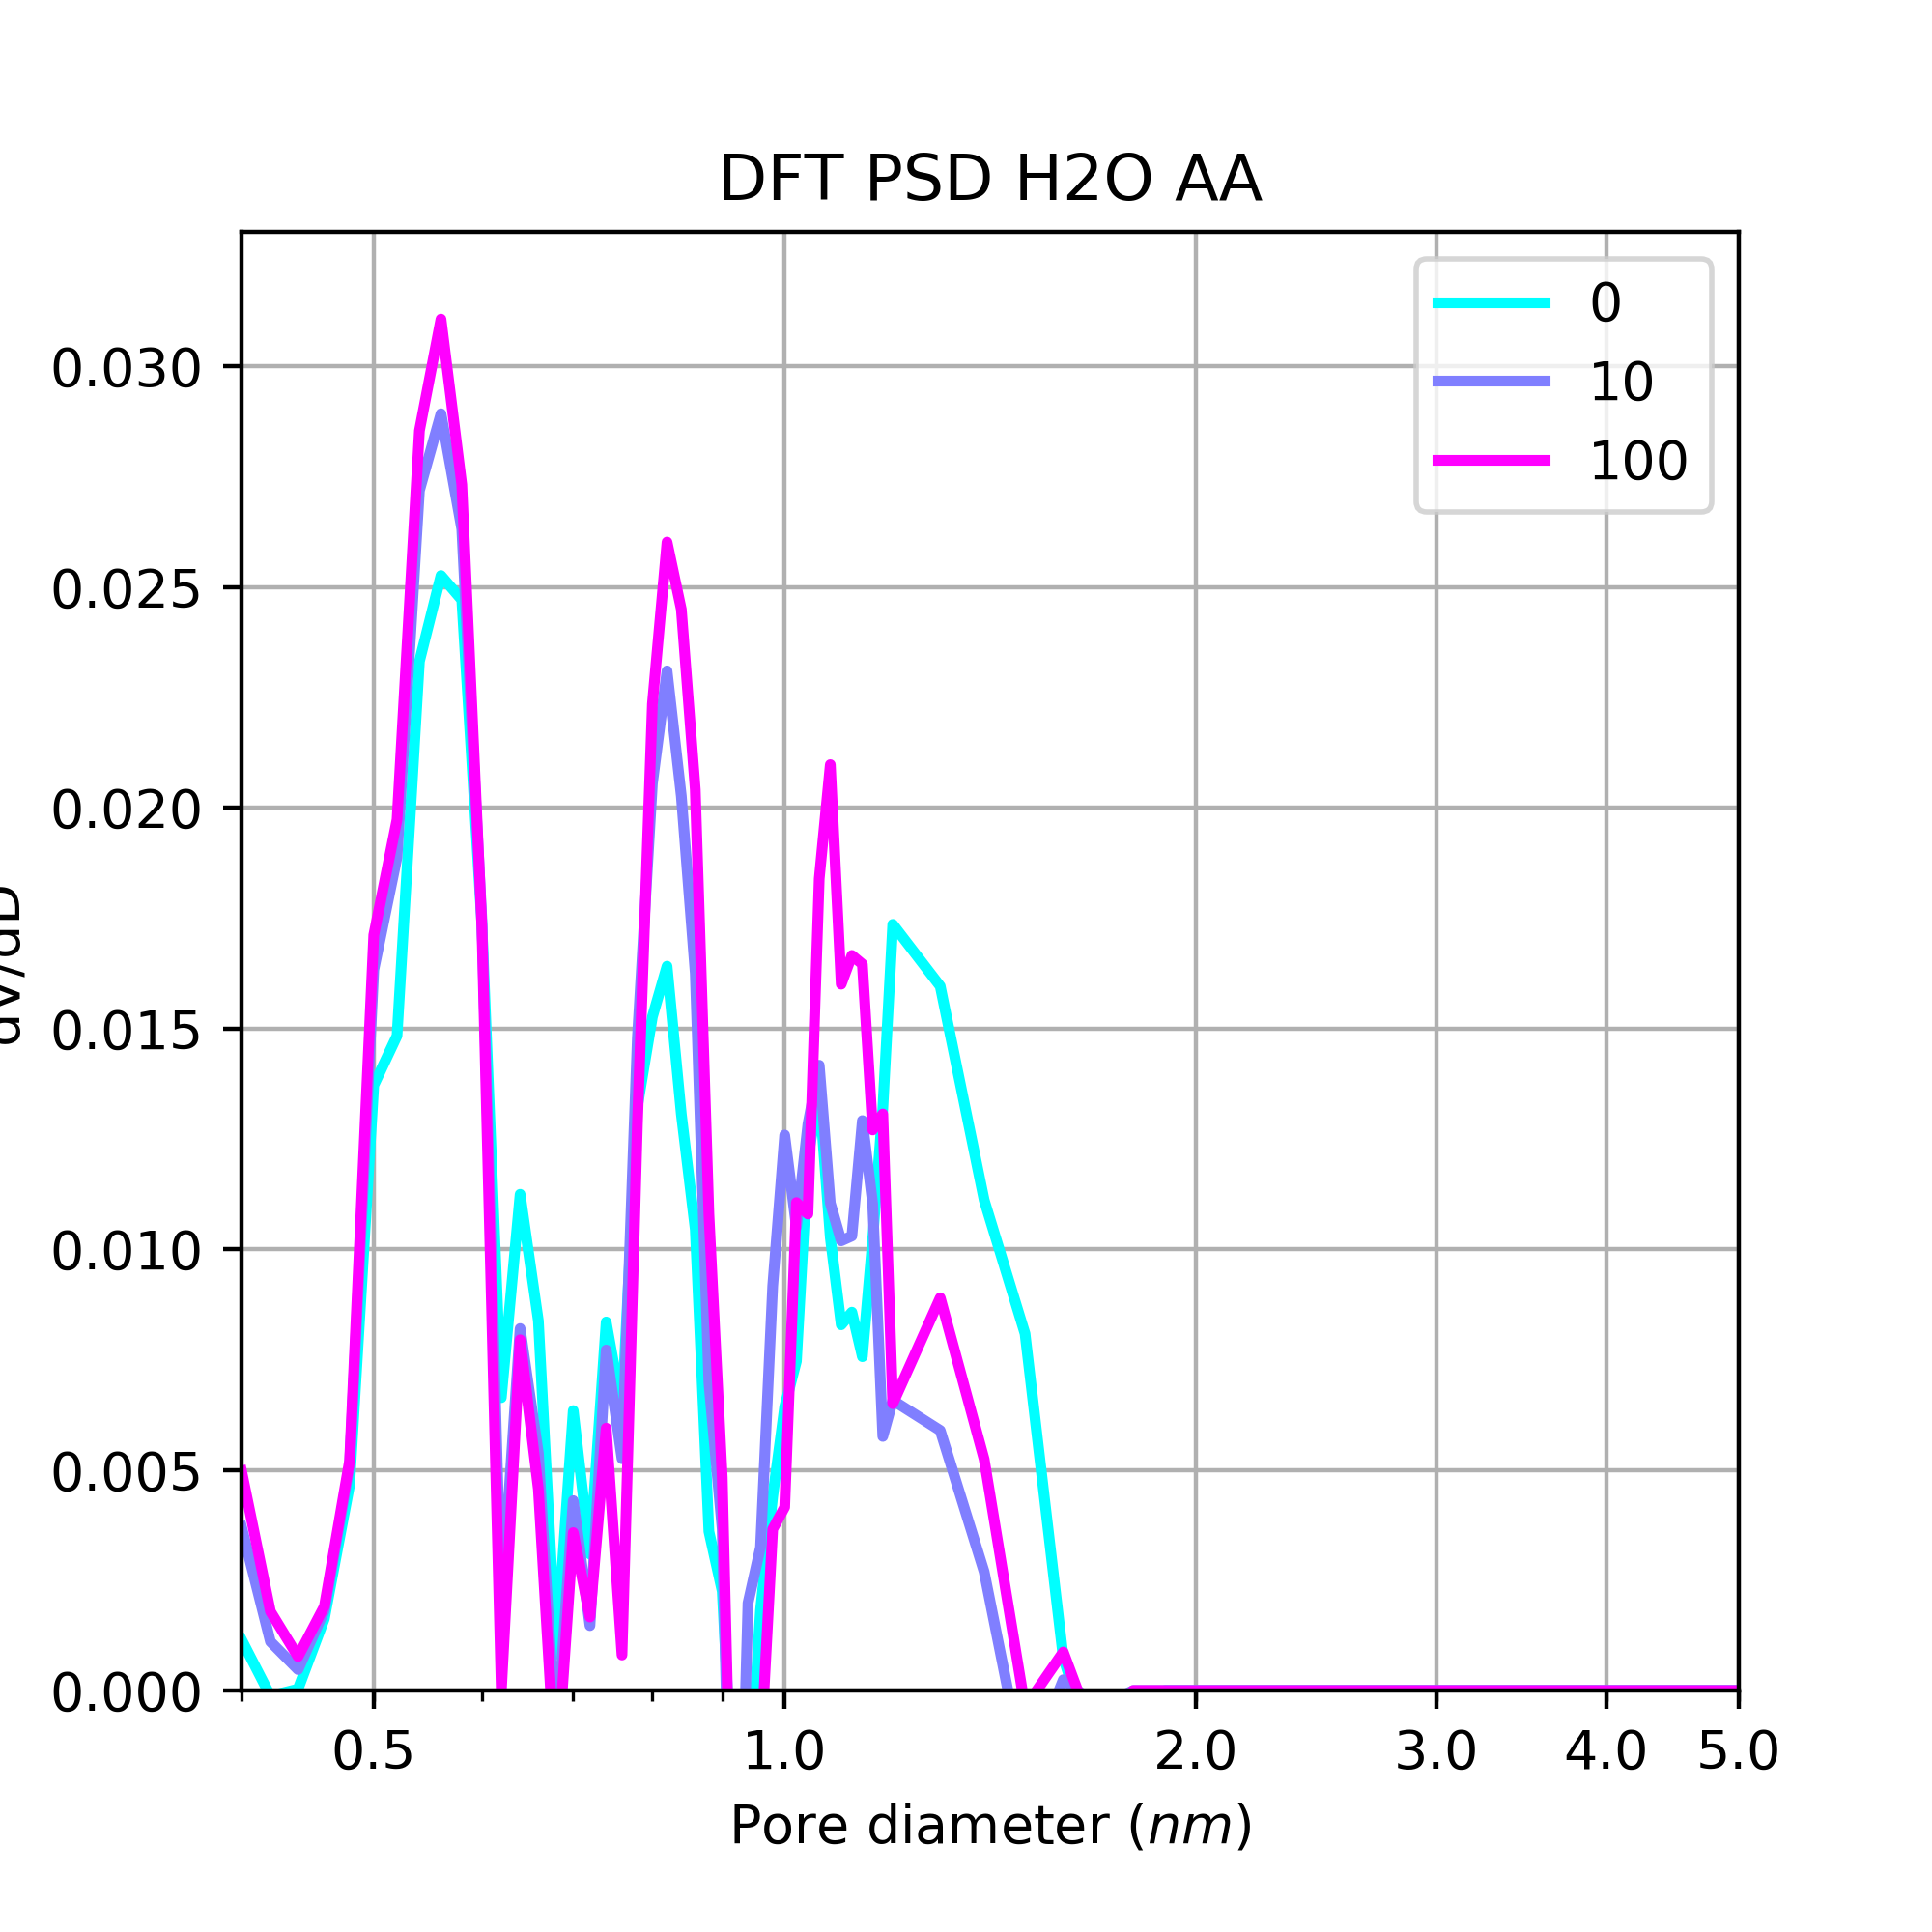
\includegraphics[width=\textwidth]{n2phys/h2o-aa-psd-dft}%
        \label{appx:def:fgr:psd-h2o-aa-dft}
    \end{subfigure}%

    \begin{subfigure}{0.25\linewidth}
        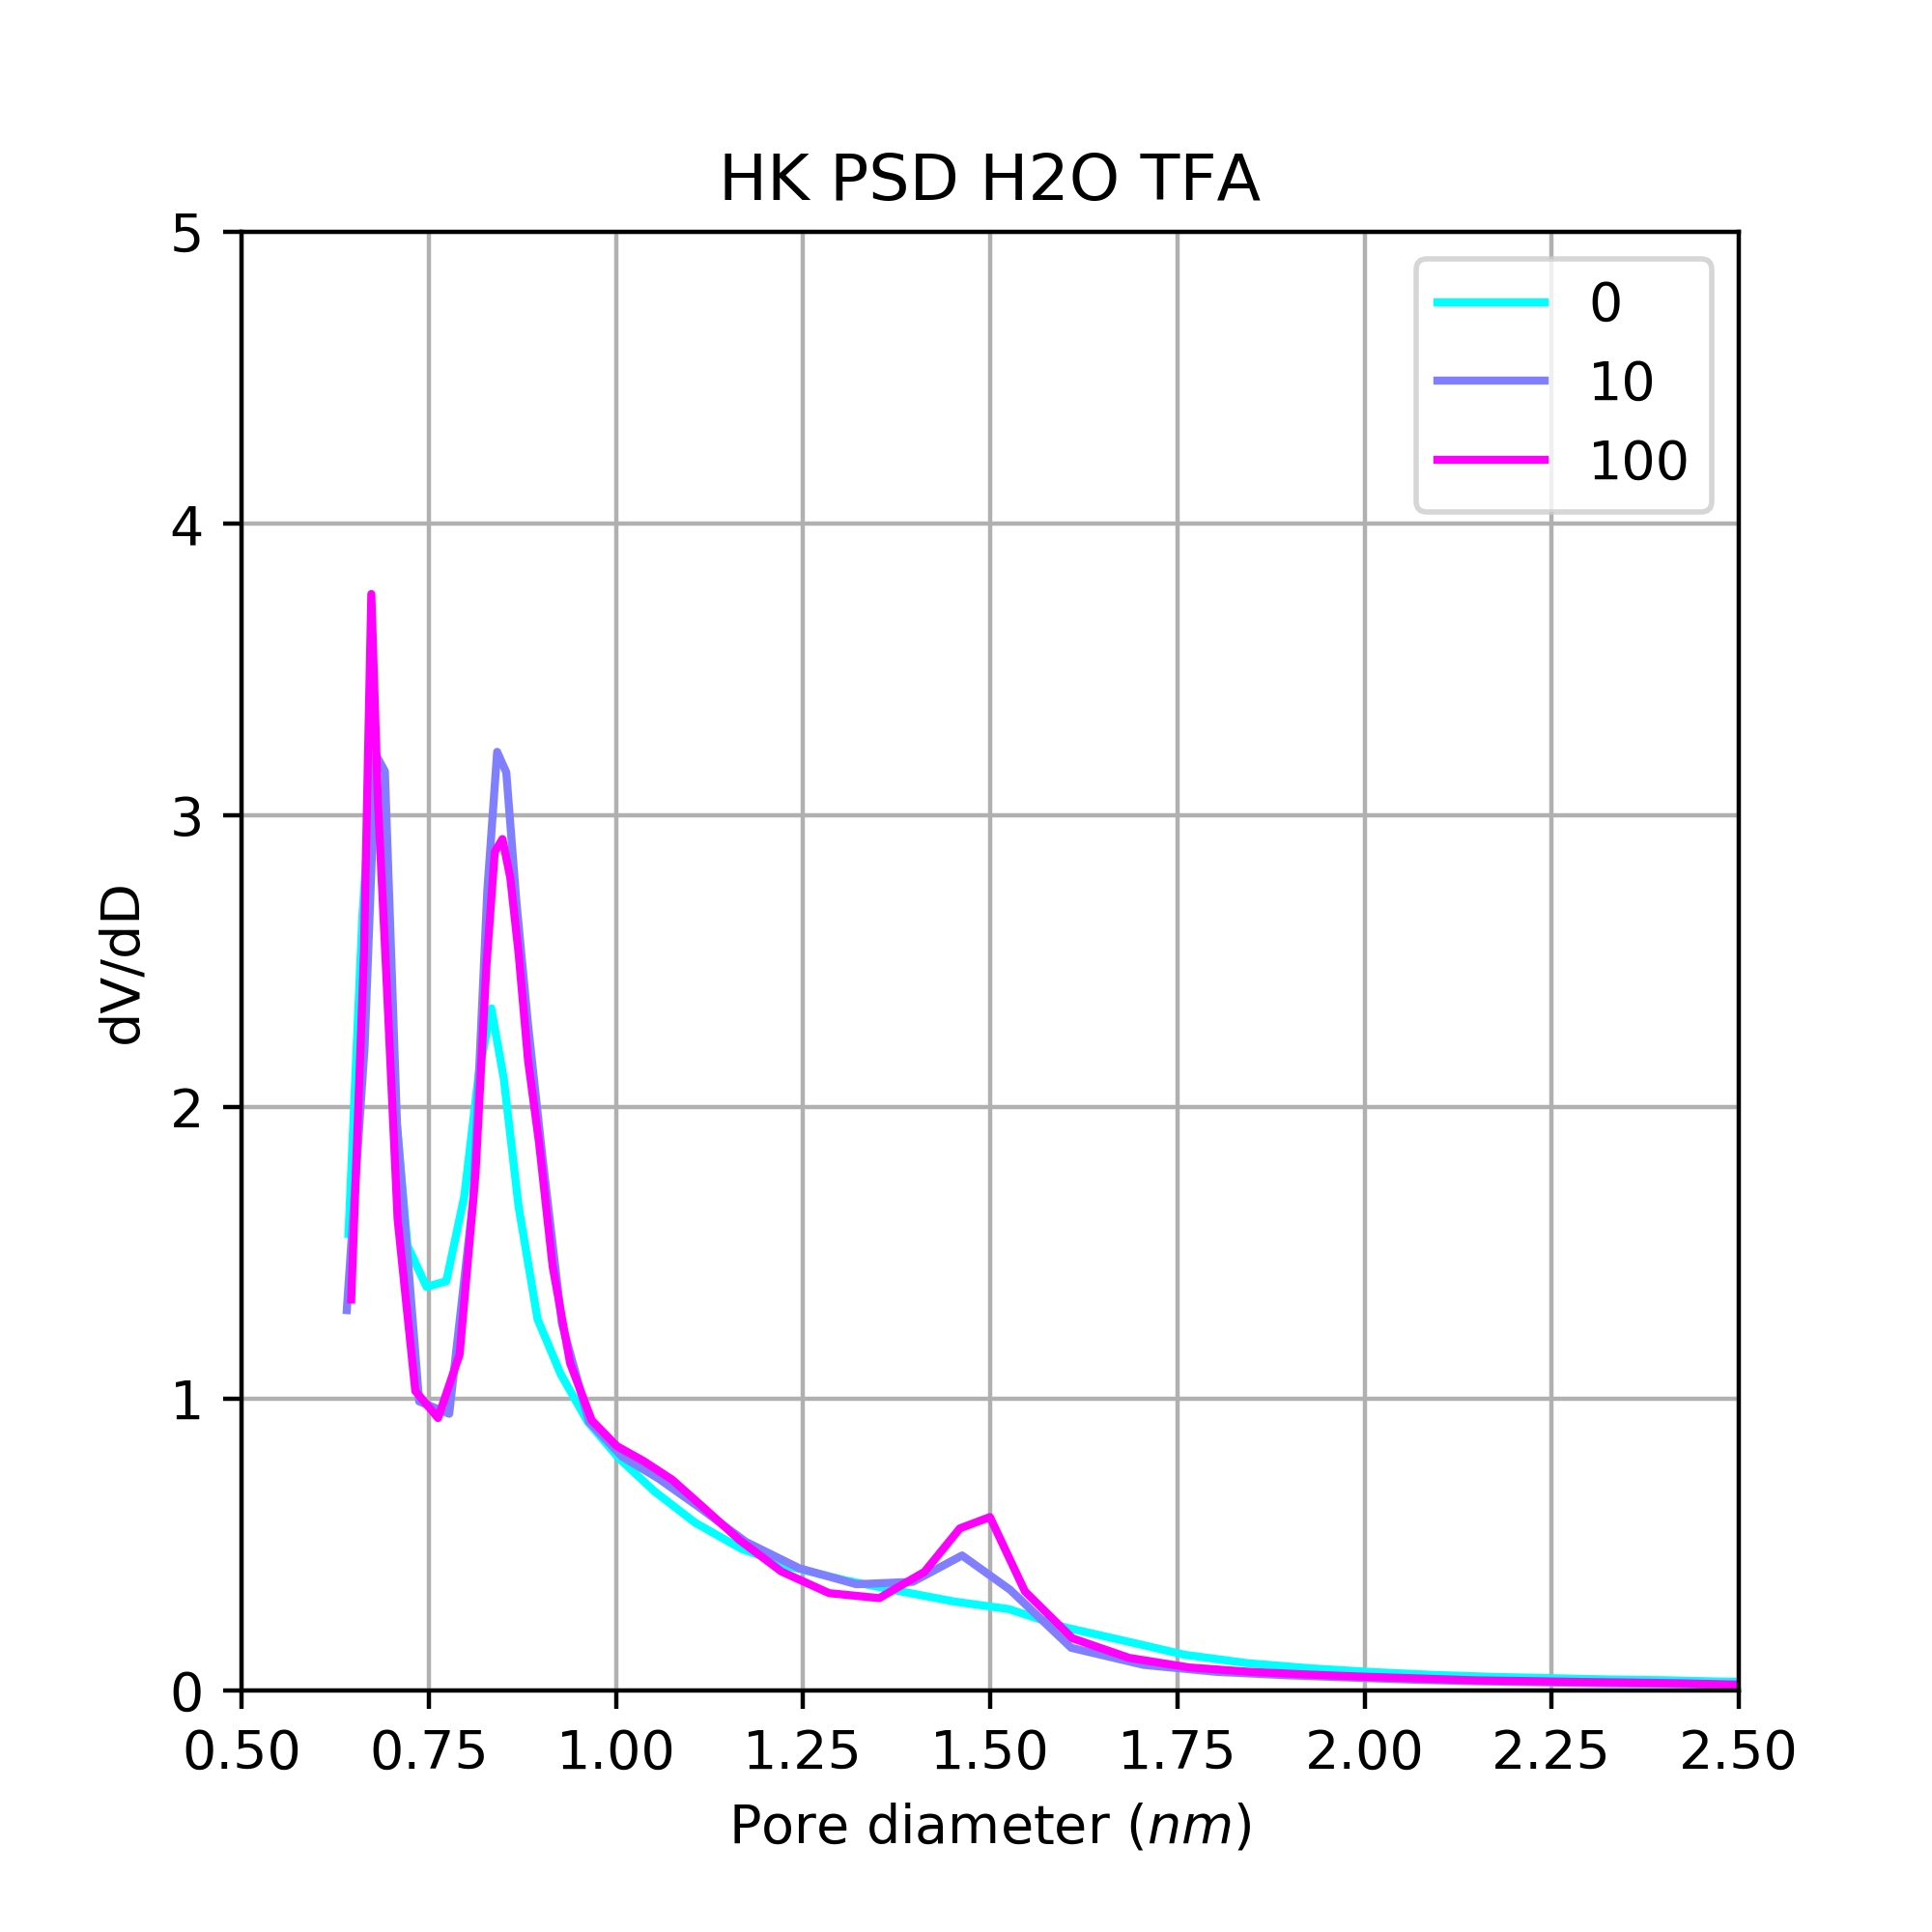
\includegraphics[width=\textwidth]{n2phys/h2o-tfa-psd-hk}%
        \label{appx:def:fgr:psd-h2o-tfa-hk}
    \end{subfigure}%
    \begin{subfigure}{0.25\linewidth}
        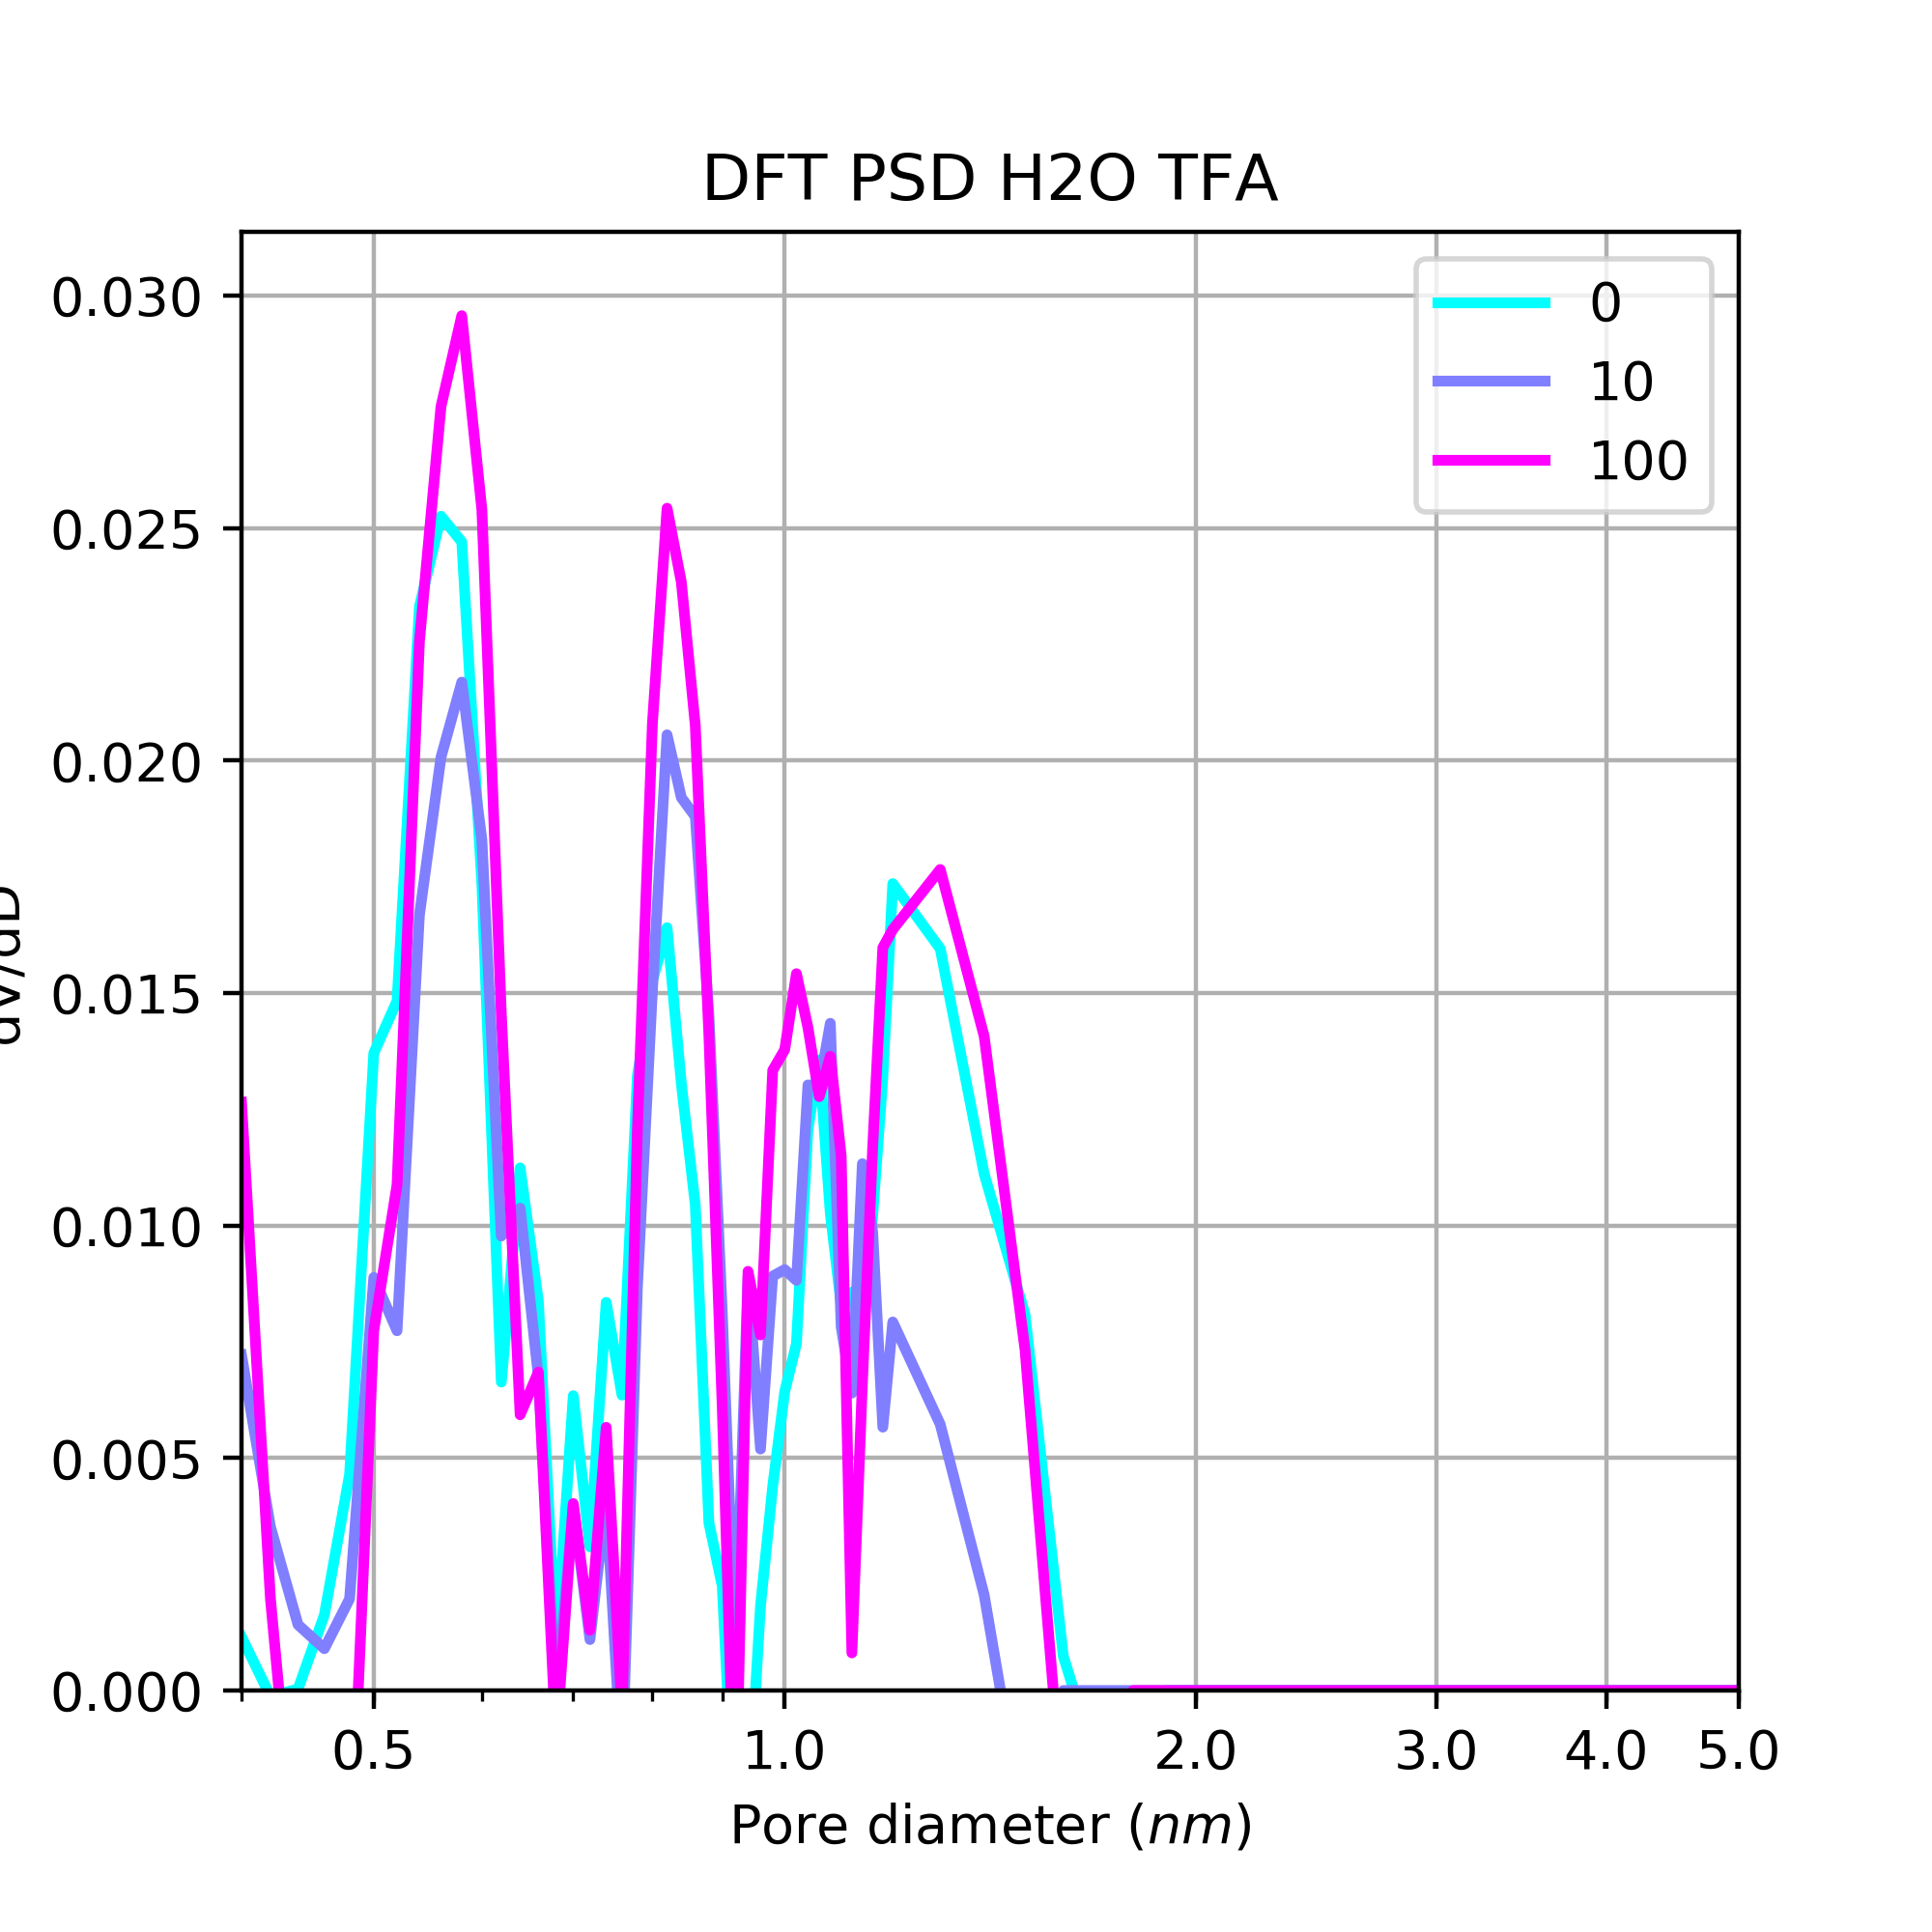
\includegraphics[width=\textwidth]{n2phys/h2o-tfa-psd-dft}%
        \label{appx:def:fgr:psd-h2o-tfa-dft}
    \end{subfigure}%
\end{figure}

\pagebreak
\begin{figure}[!h]\ContinuedFloat{}
    \centering
    
    \begin{subfigure}{0.25\linewidth}
        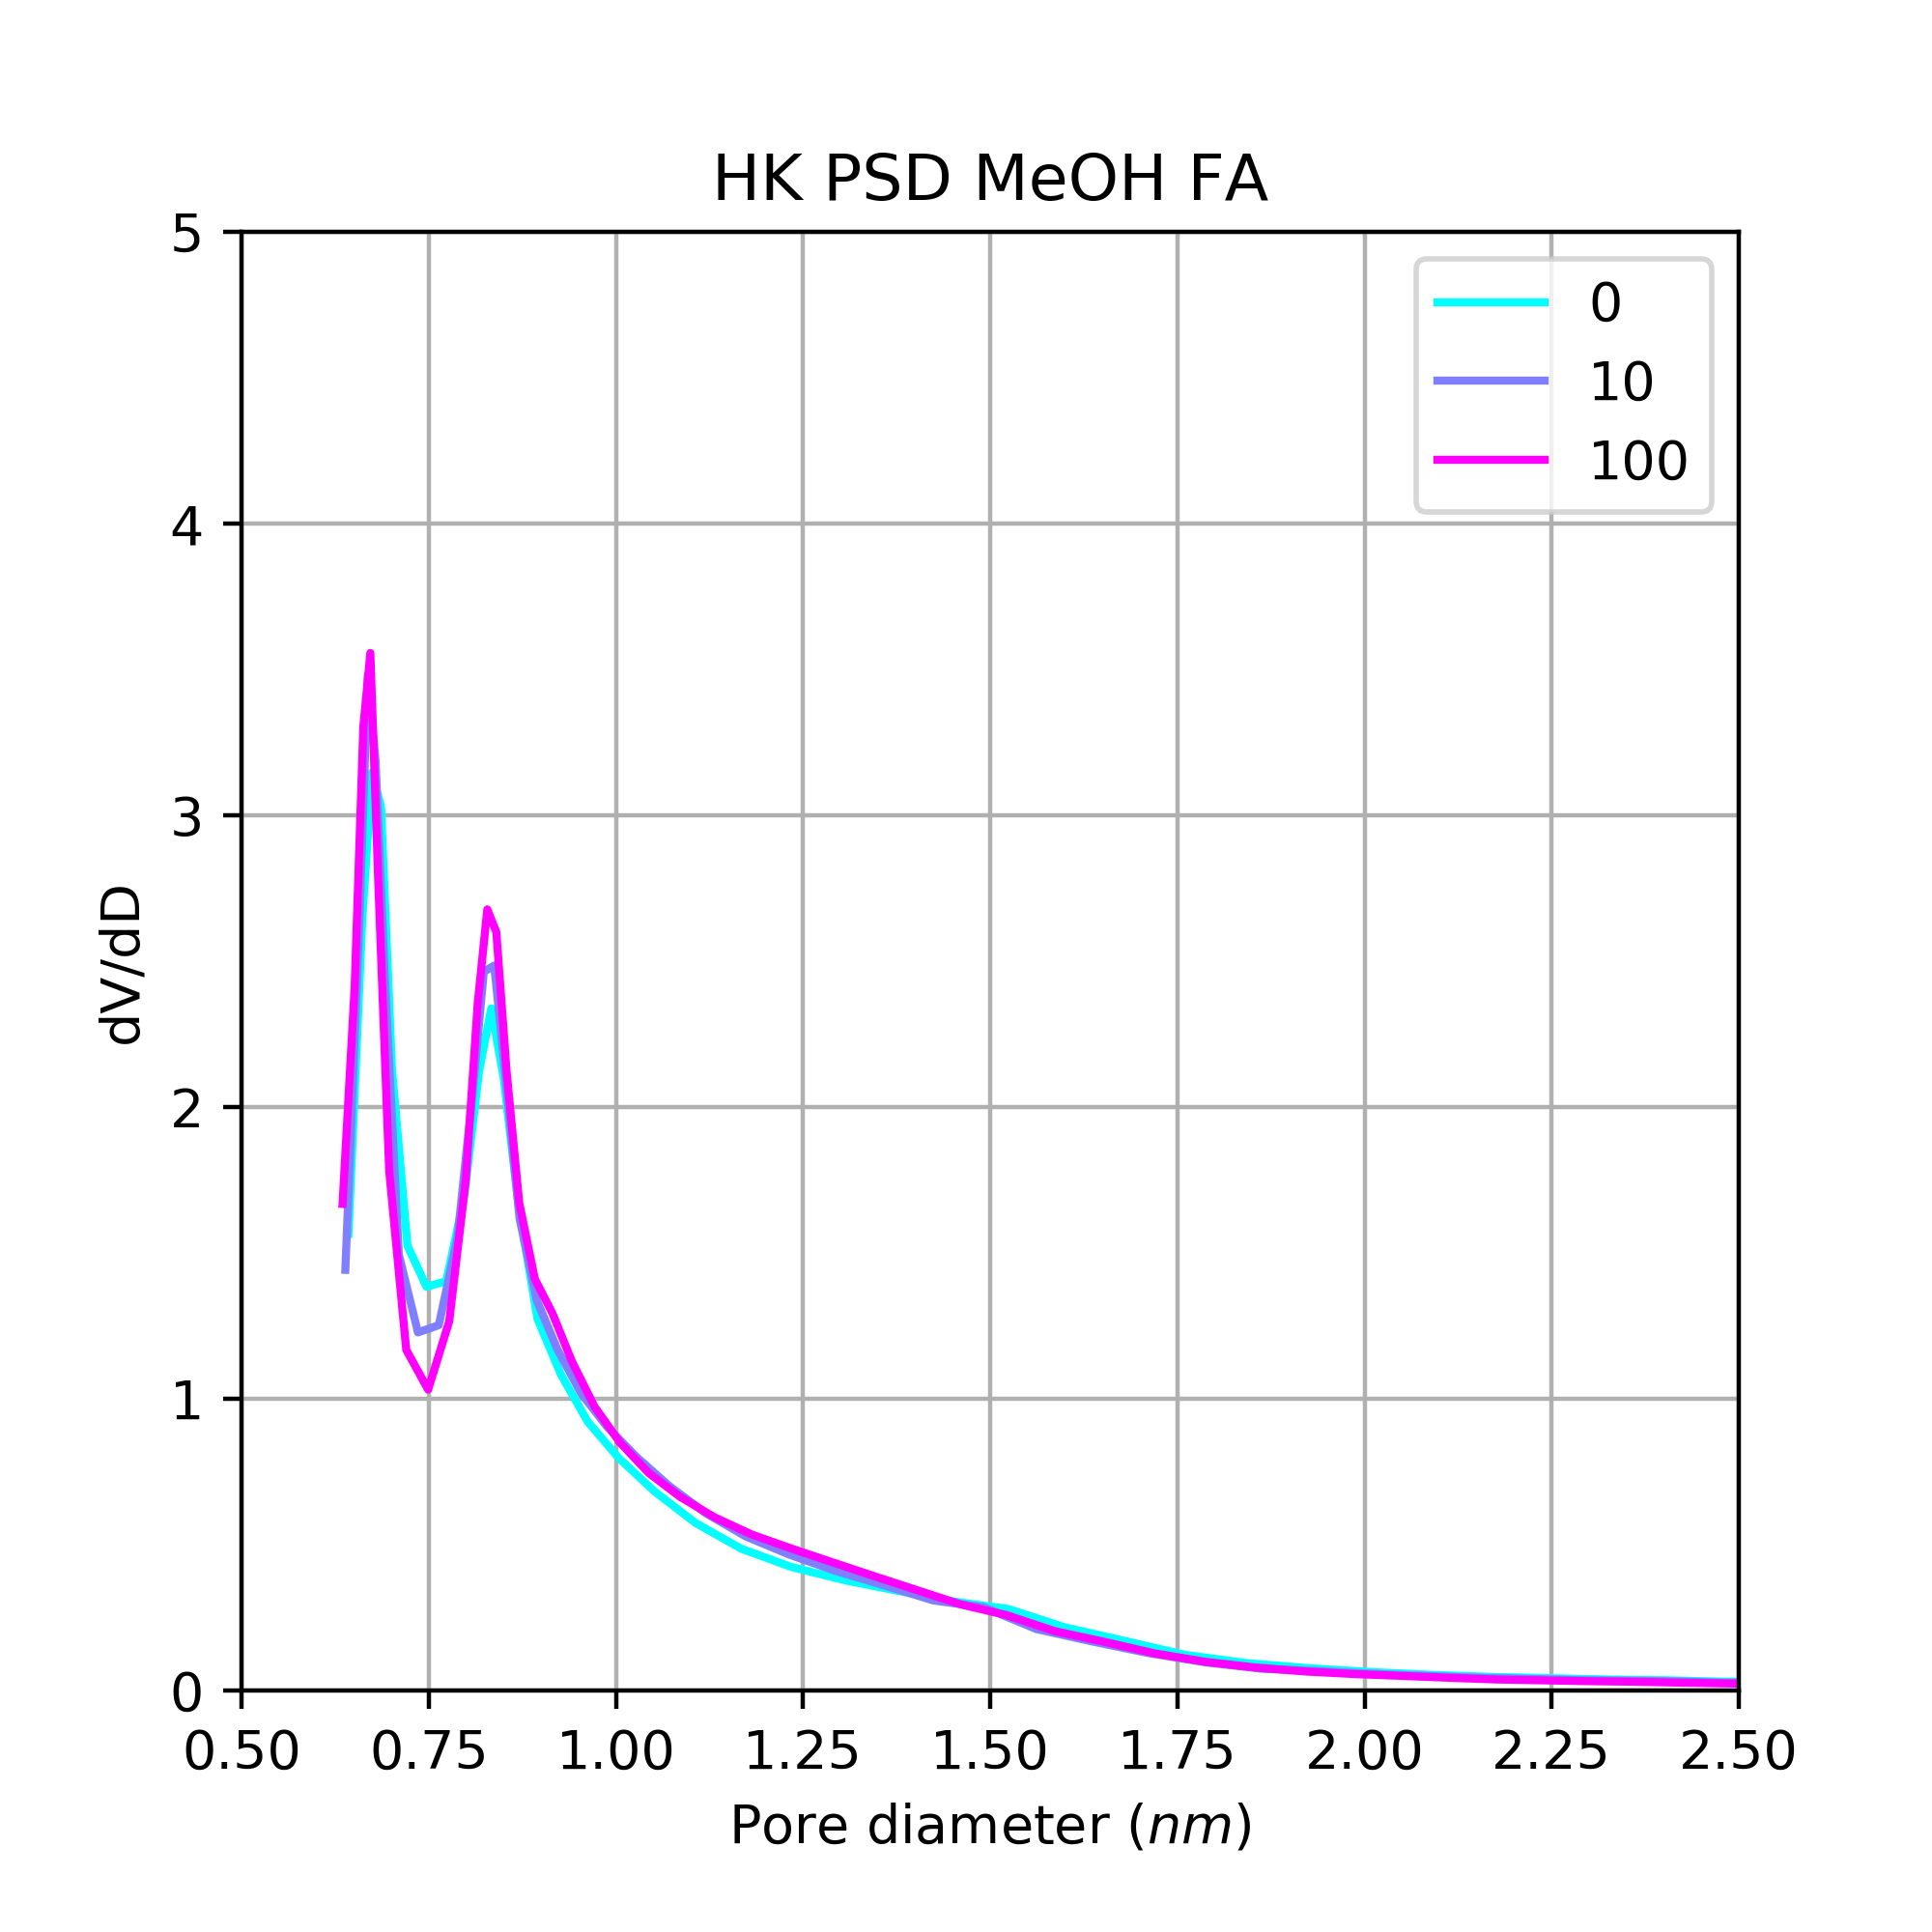
\includegraphics[width=\textwidth]{n2phys/meoh-fa-psd-hk}%
        \label{appx:def:fgr:psd-meoh-fa-hk}
    \end{subfigure}%
    \begin{subfigure}{0.25\linewidth}
        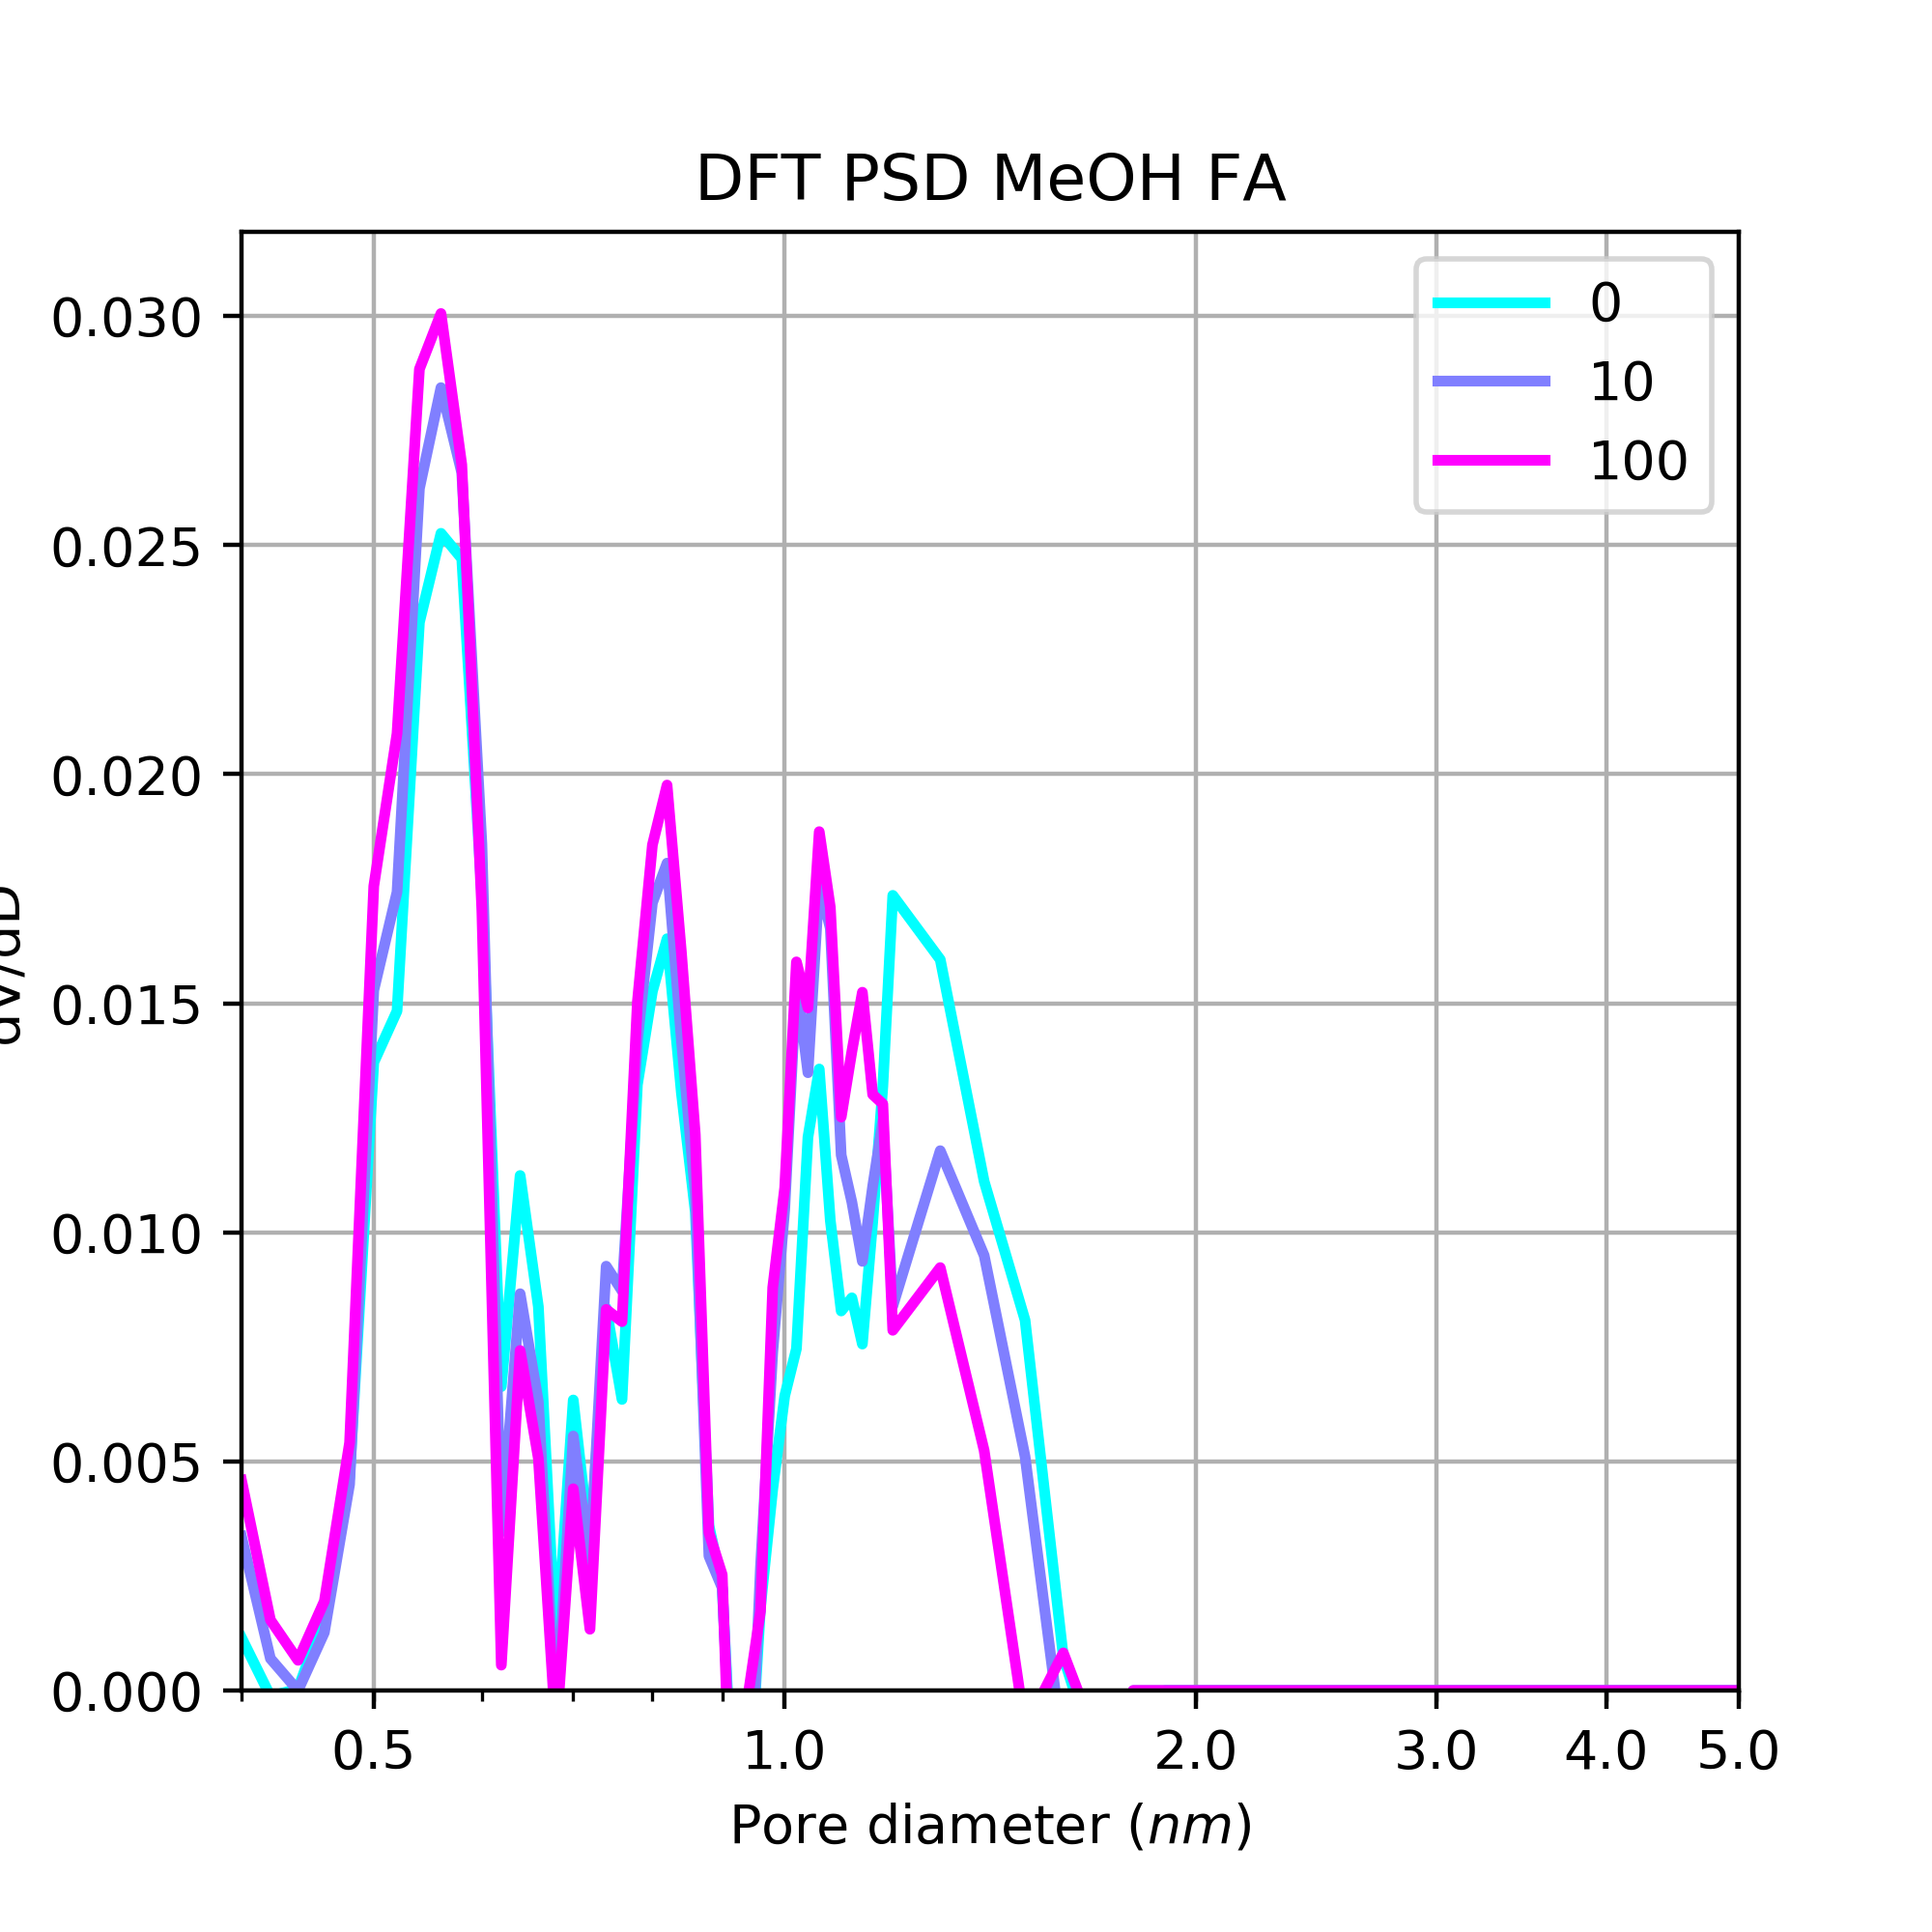
\includegraphics[width=\textwidth]{n2phys/meoh-fa-psd-dft}%
        \label{appx:def:fgr:psd-meoh-fa-dft}
    \end{subfigure}%
    \begin{subfigure}{0.25\linewidth}
        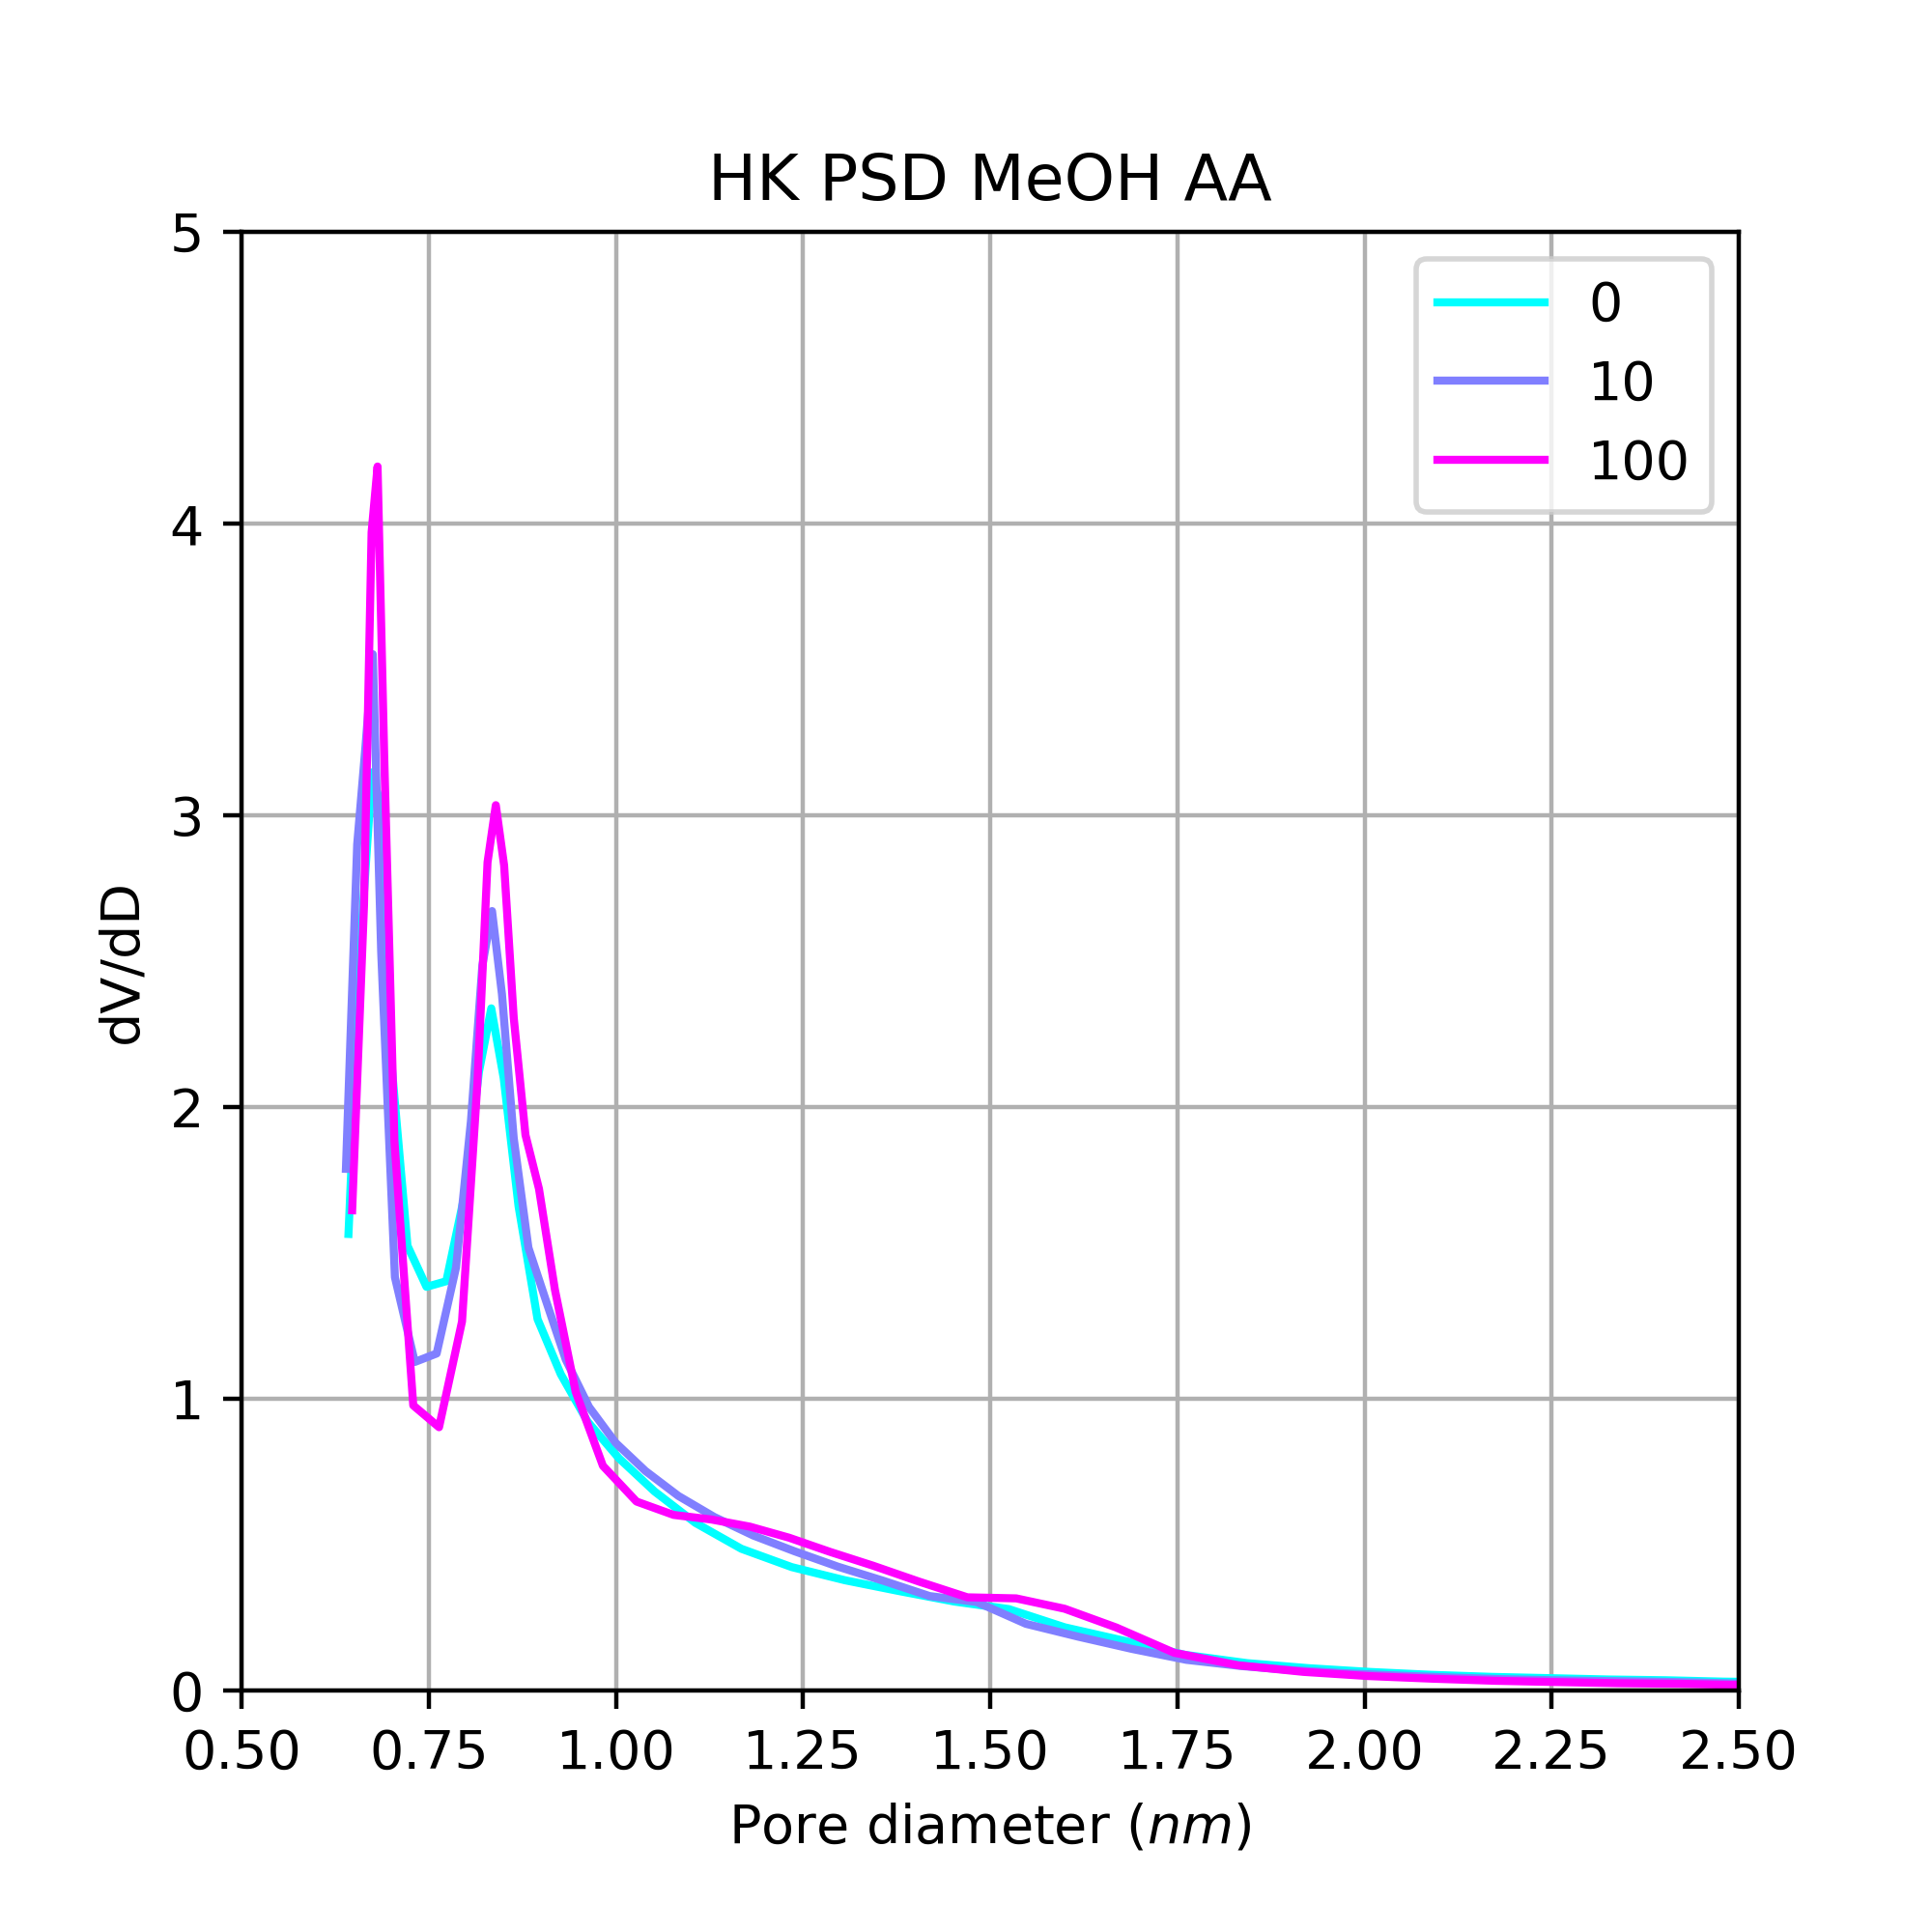
\includegraphics[width=\textwidth]{n2phys/meoh-aa-psd-hk}%
        \label{appx:def:fgr:psd-meoh-aa-hk}
    \end{subfigure}%
    \begin{subfigure}{0.25\linewidth}
        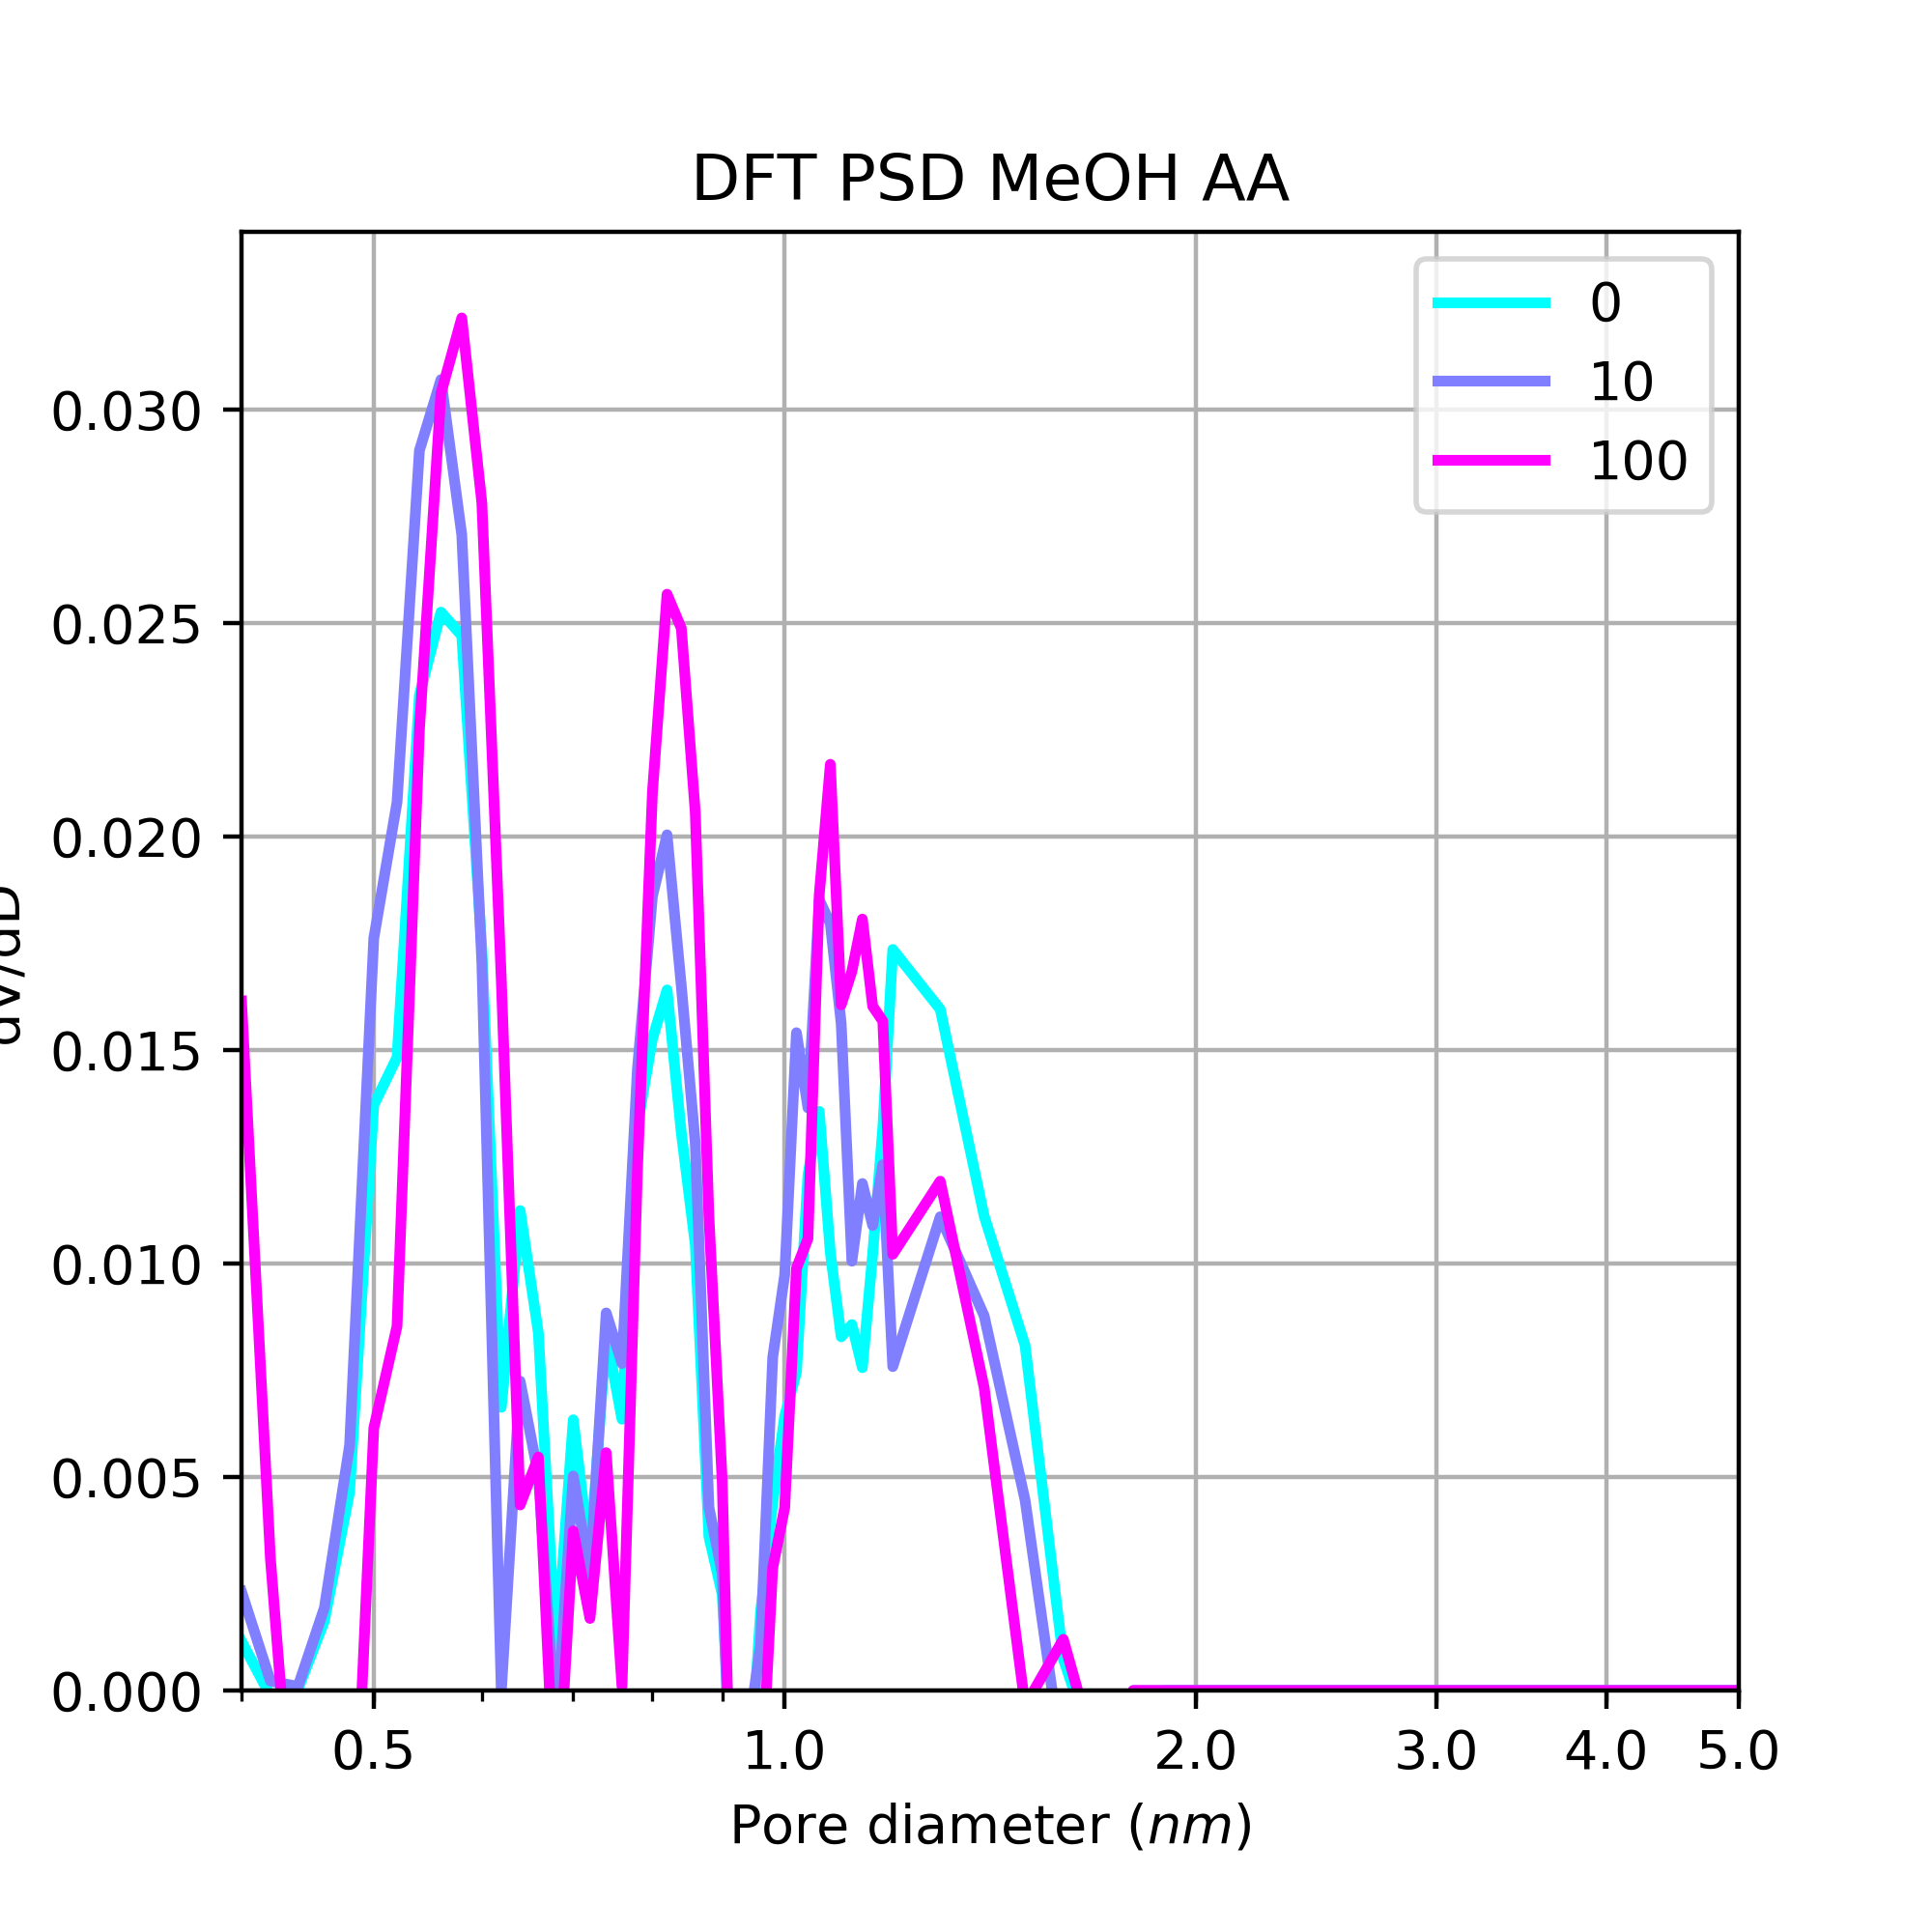
\includegraphics[width=\textwidth]{n2phys/meoh-aa-psd-dft}%
        \label{appx:def:fgr:psd-meoh-aa-dft}
    \end{subfigure}%

    \begin{subfigure}{0.25\linewidth}
        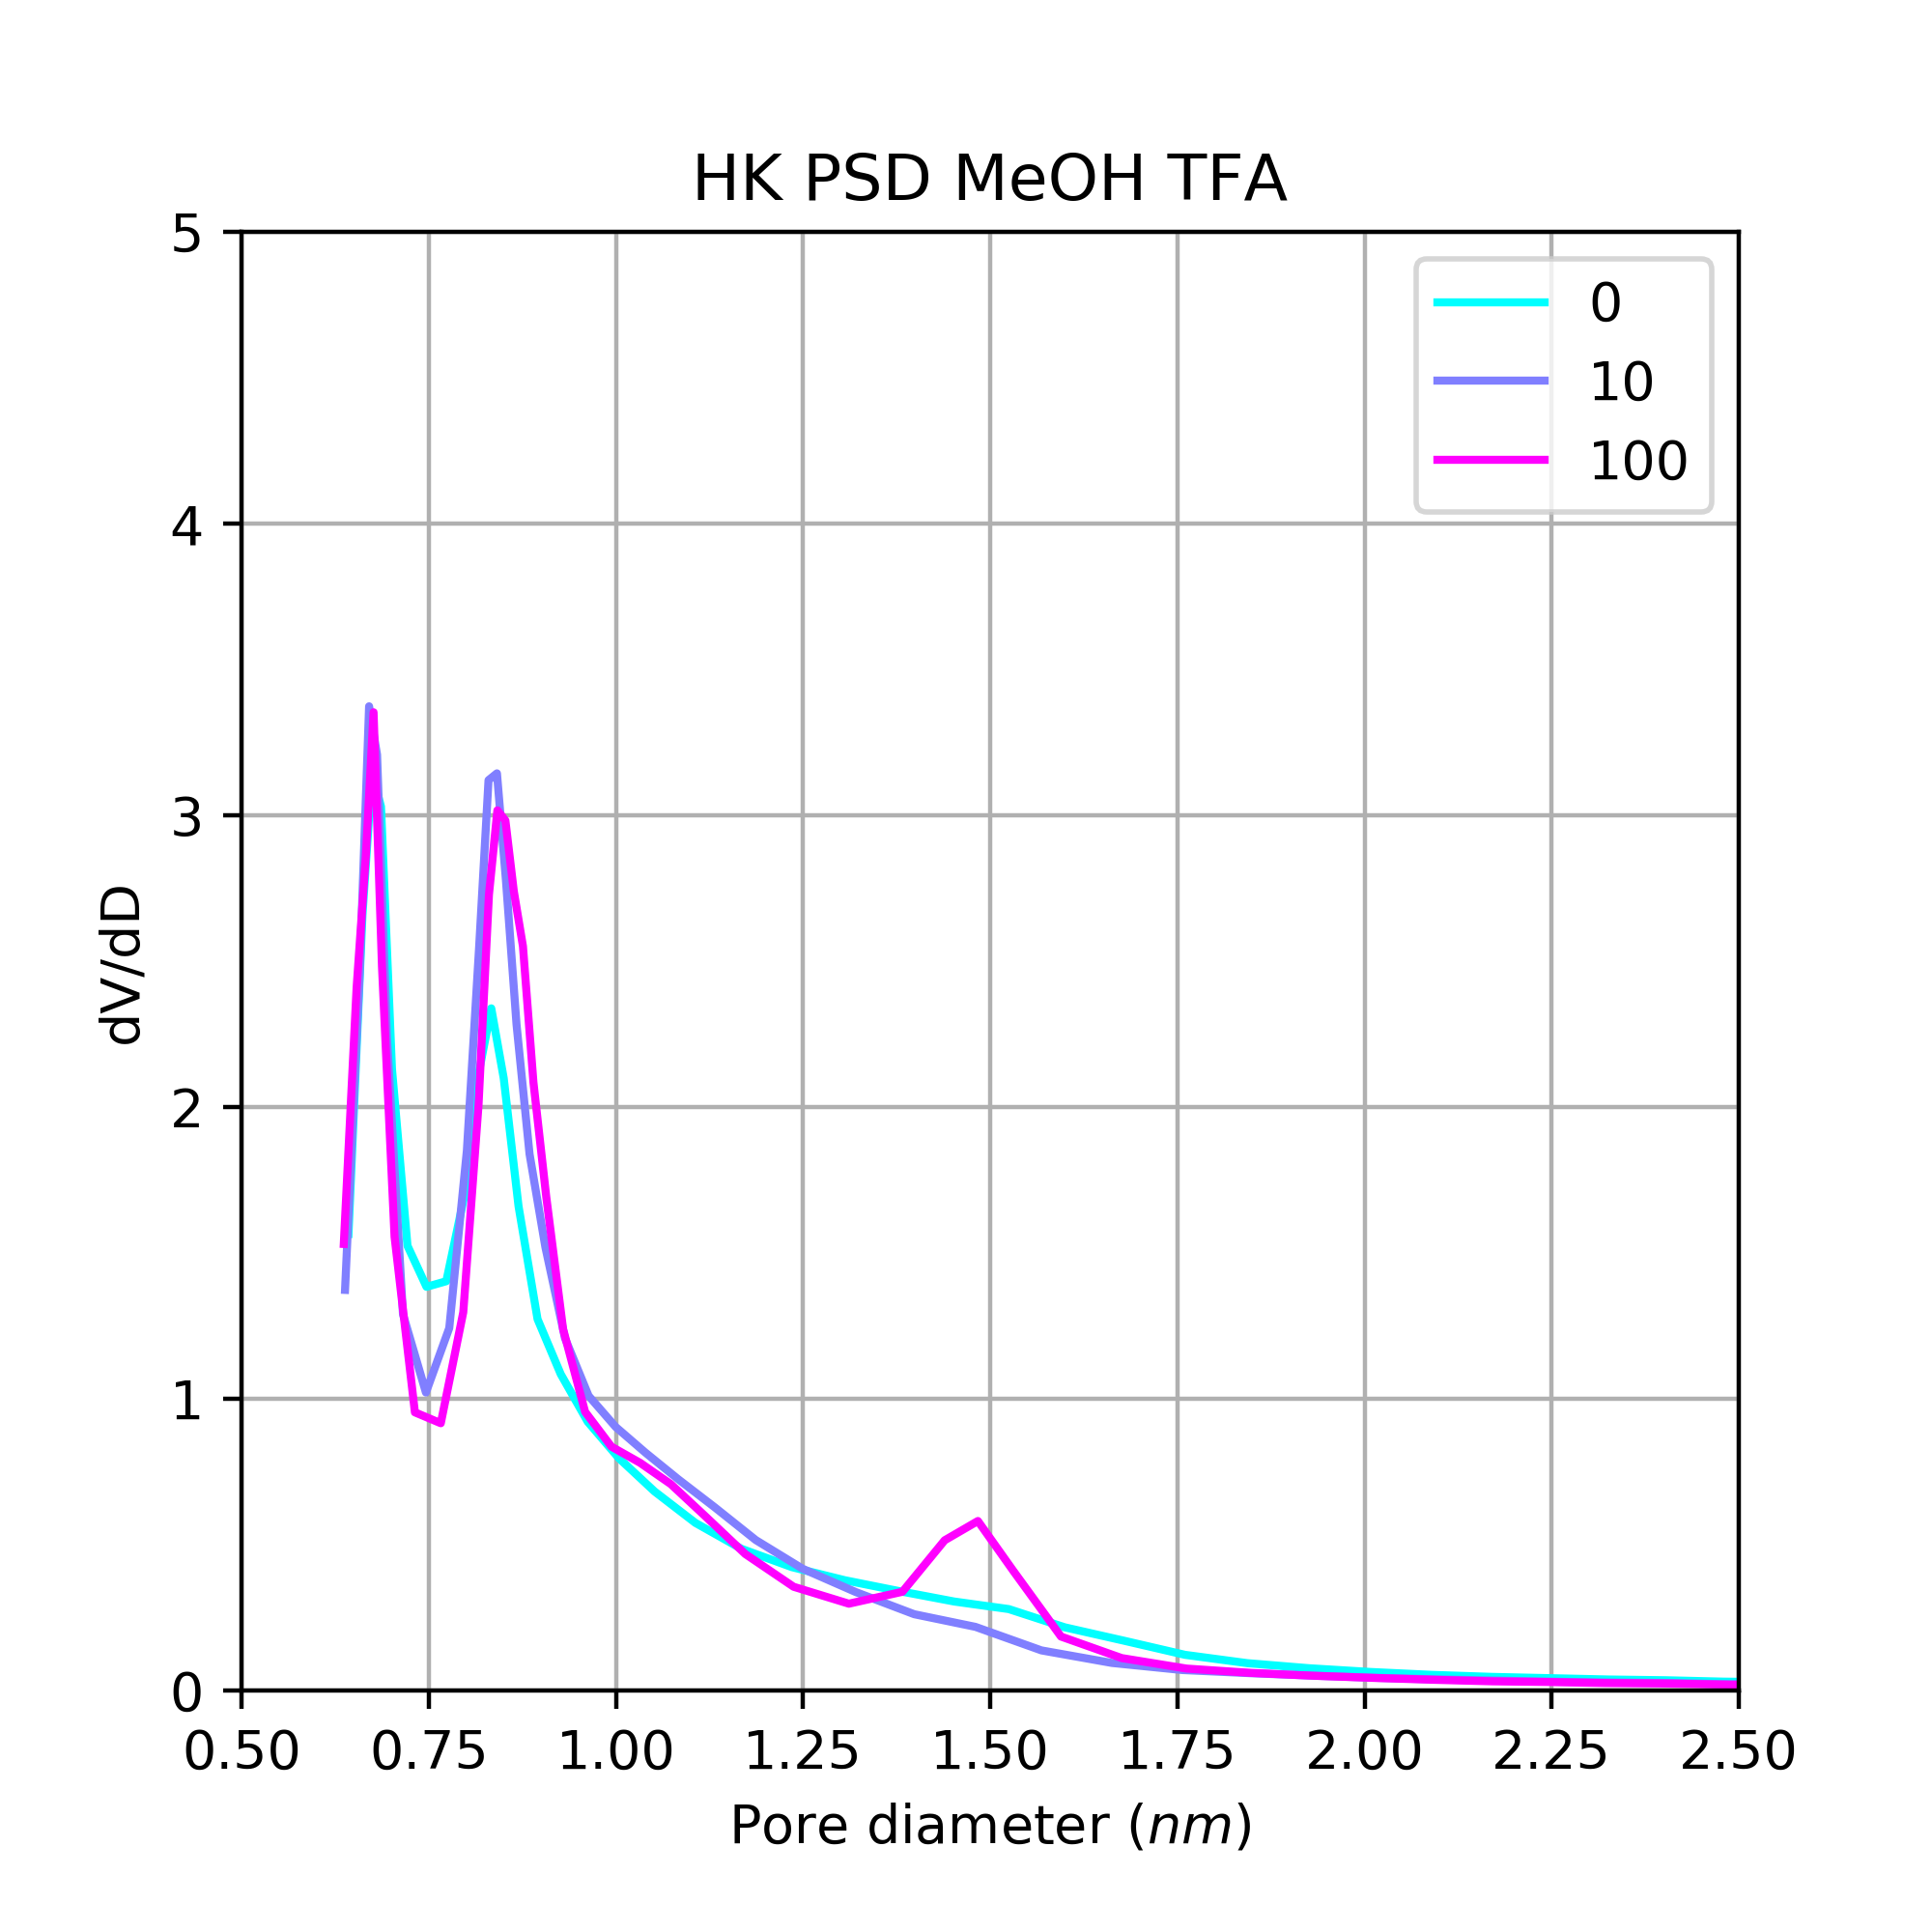
\includegraphics[width=\textwidth]{n2phys/meoh-tfa-psd-hk}%
        \label{appx:def:fgr:psd-meoh-tfa-hk}
    \end{subfigure}%
    \begin{subfigure}{0.25\linewidth}
        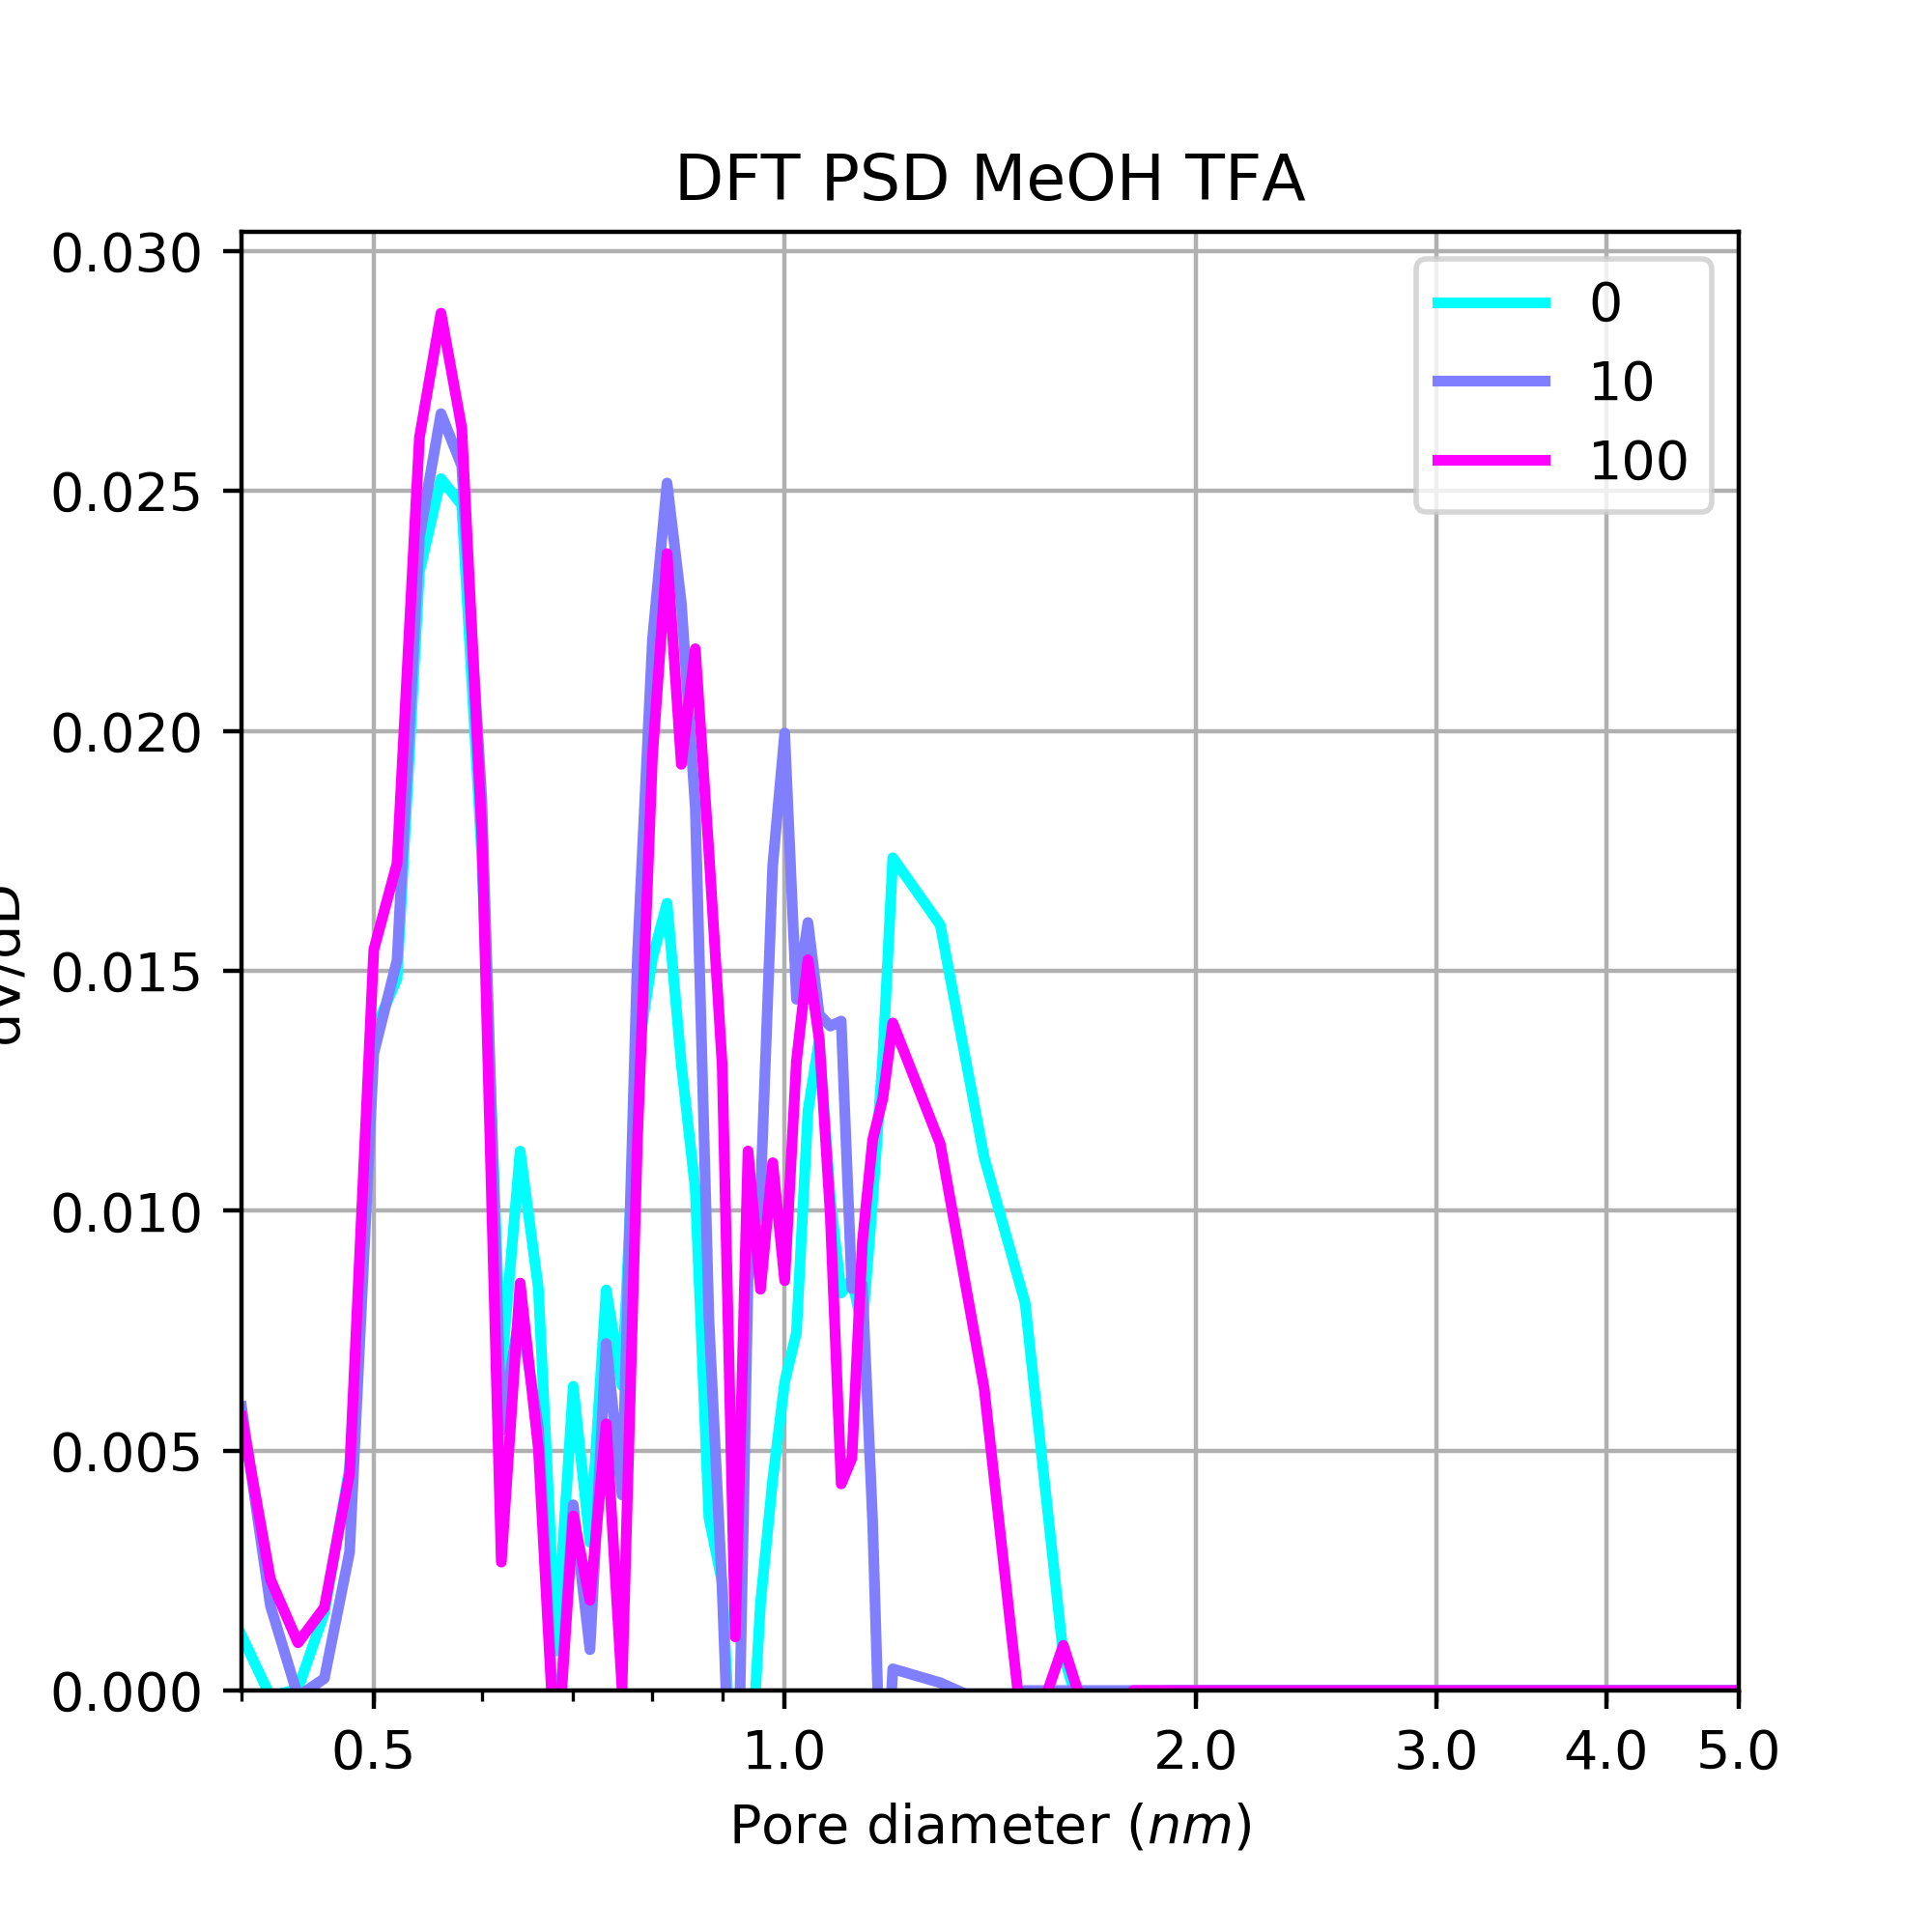
\includegraphics[width=\textwidth]{n2phys/meoh-tfa-psd-dft}%
        \label{appx:def:fgr:psd-meoh-tfa-dft}
    \end{subfigure}%
    \begin{subfigure}{0.25\linewidth}
        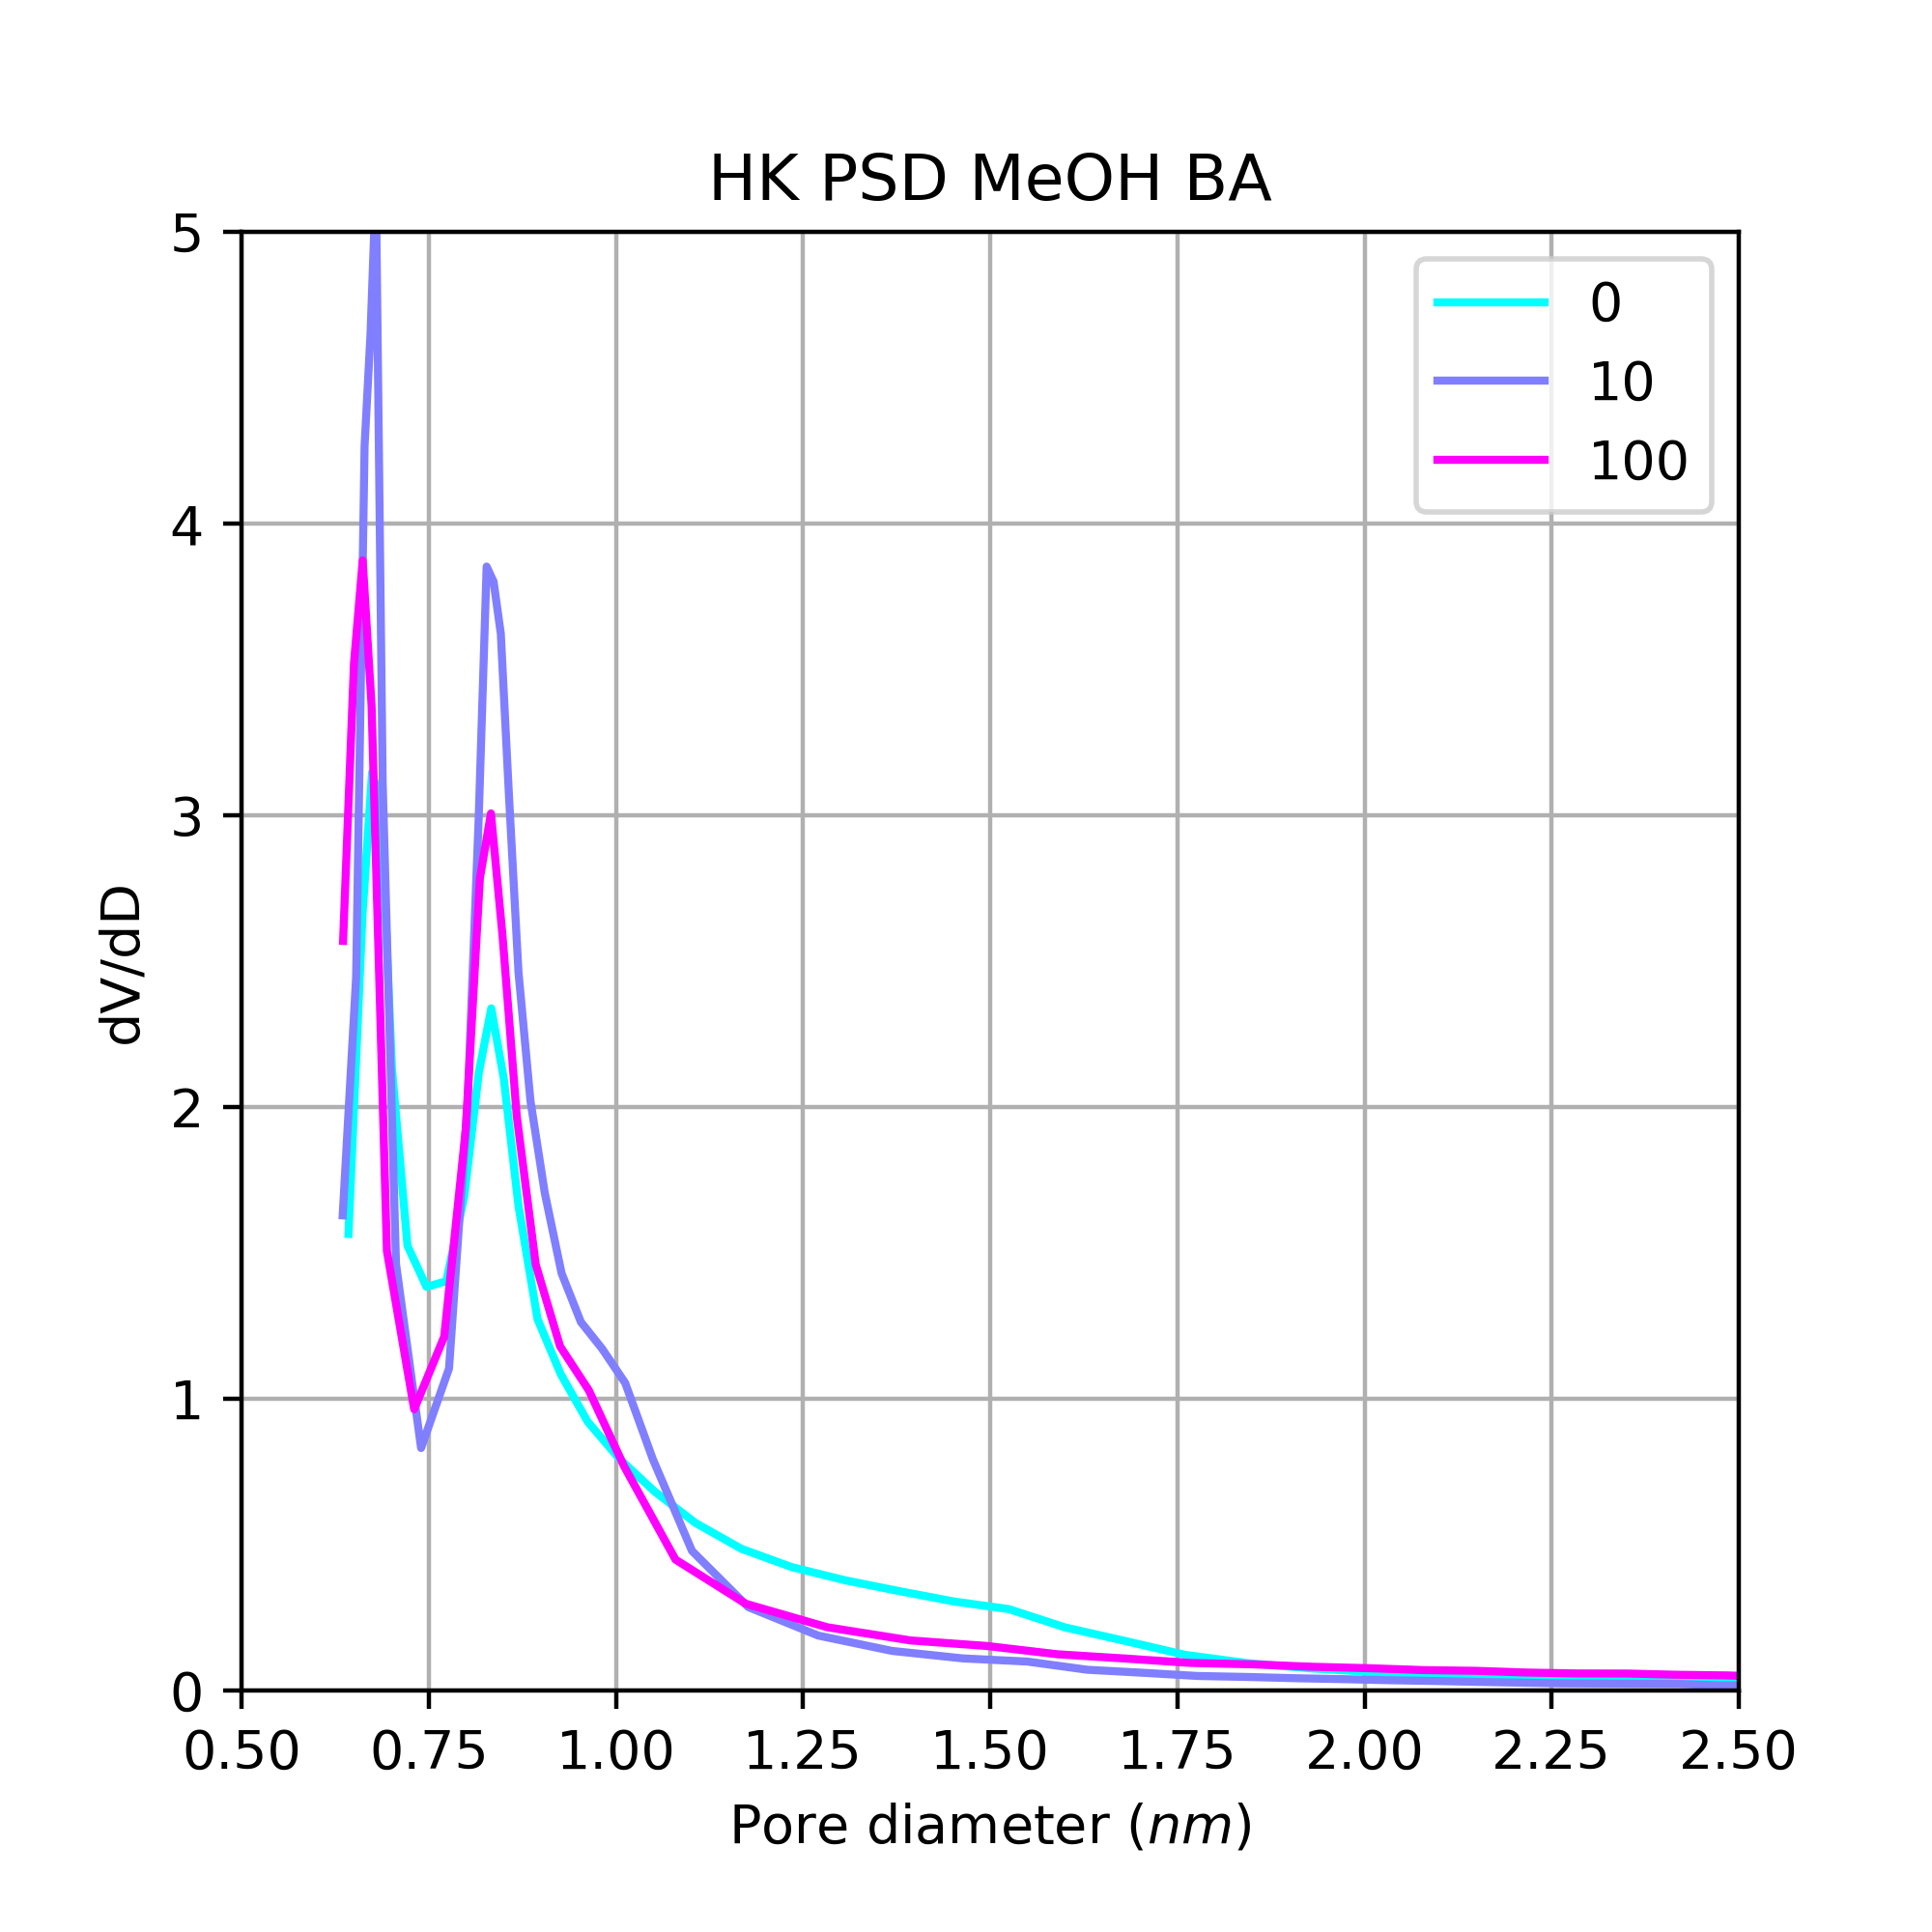
\includegraphics[width=\textwidth]{n2phys/meoh-ba-psd-hk}%
        \label{appx:def:fgr:psd-meoh-ba-hk}
    \end{subfigure}%
    \begin{subfigure}{0.25\linewidth}
        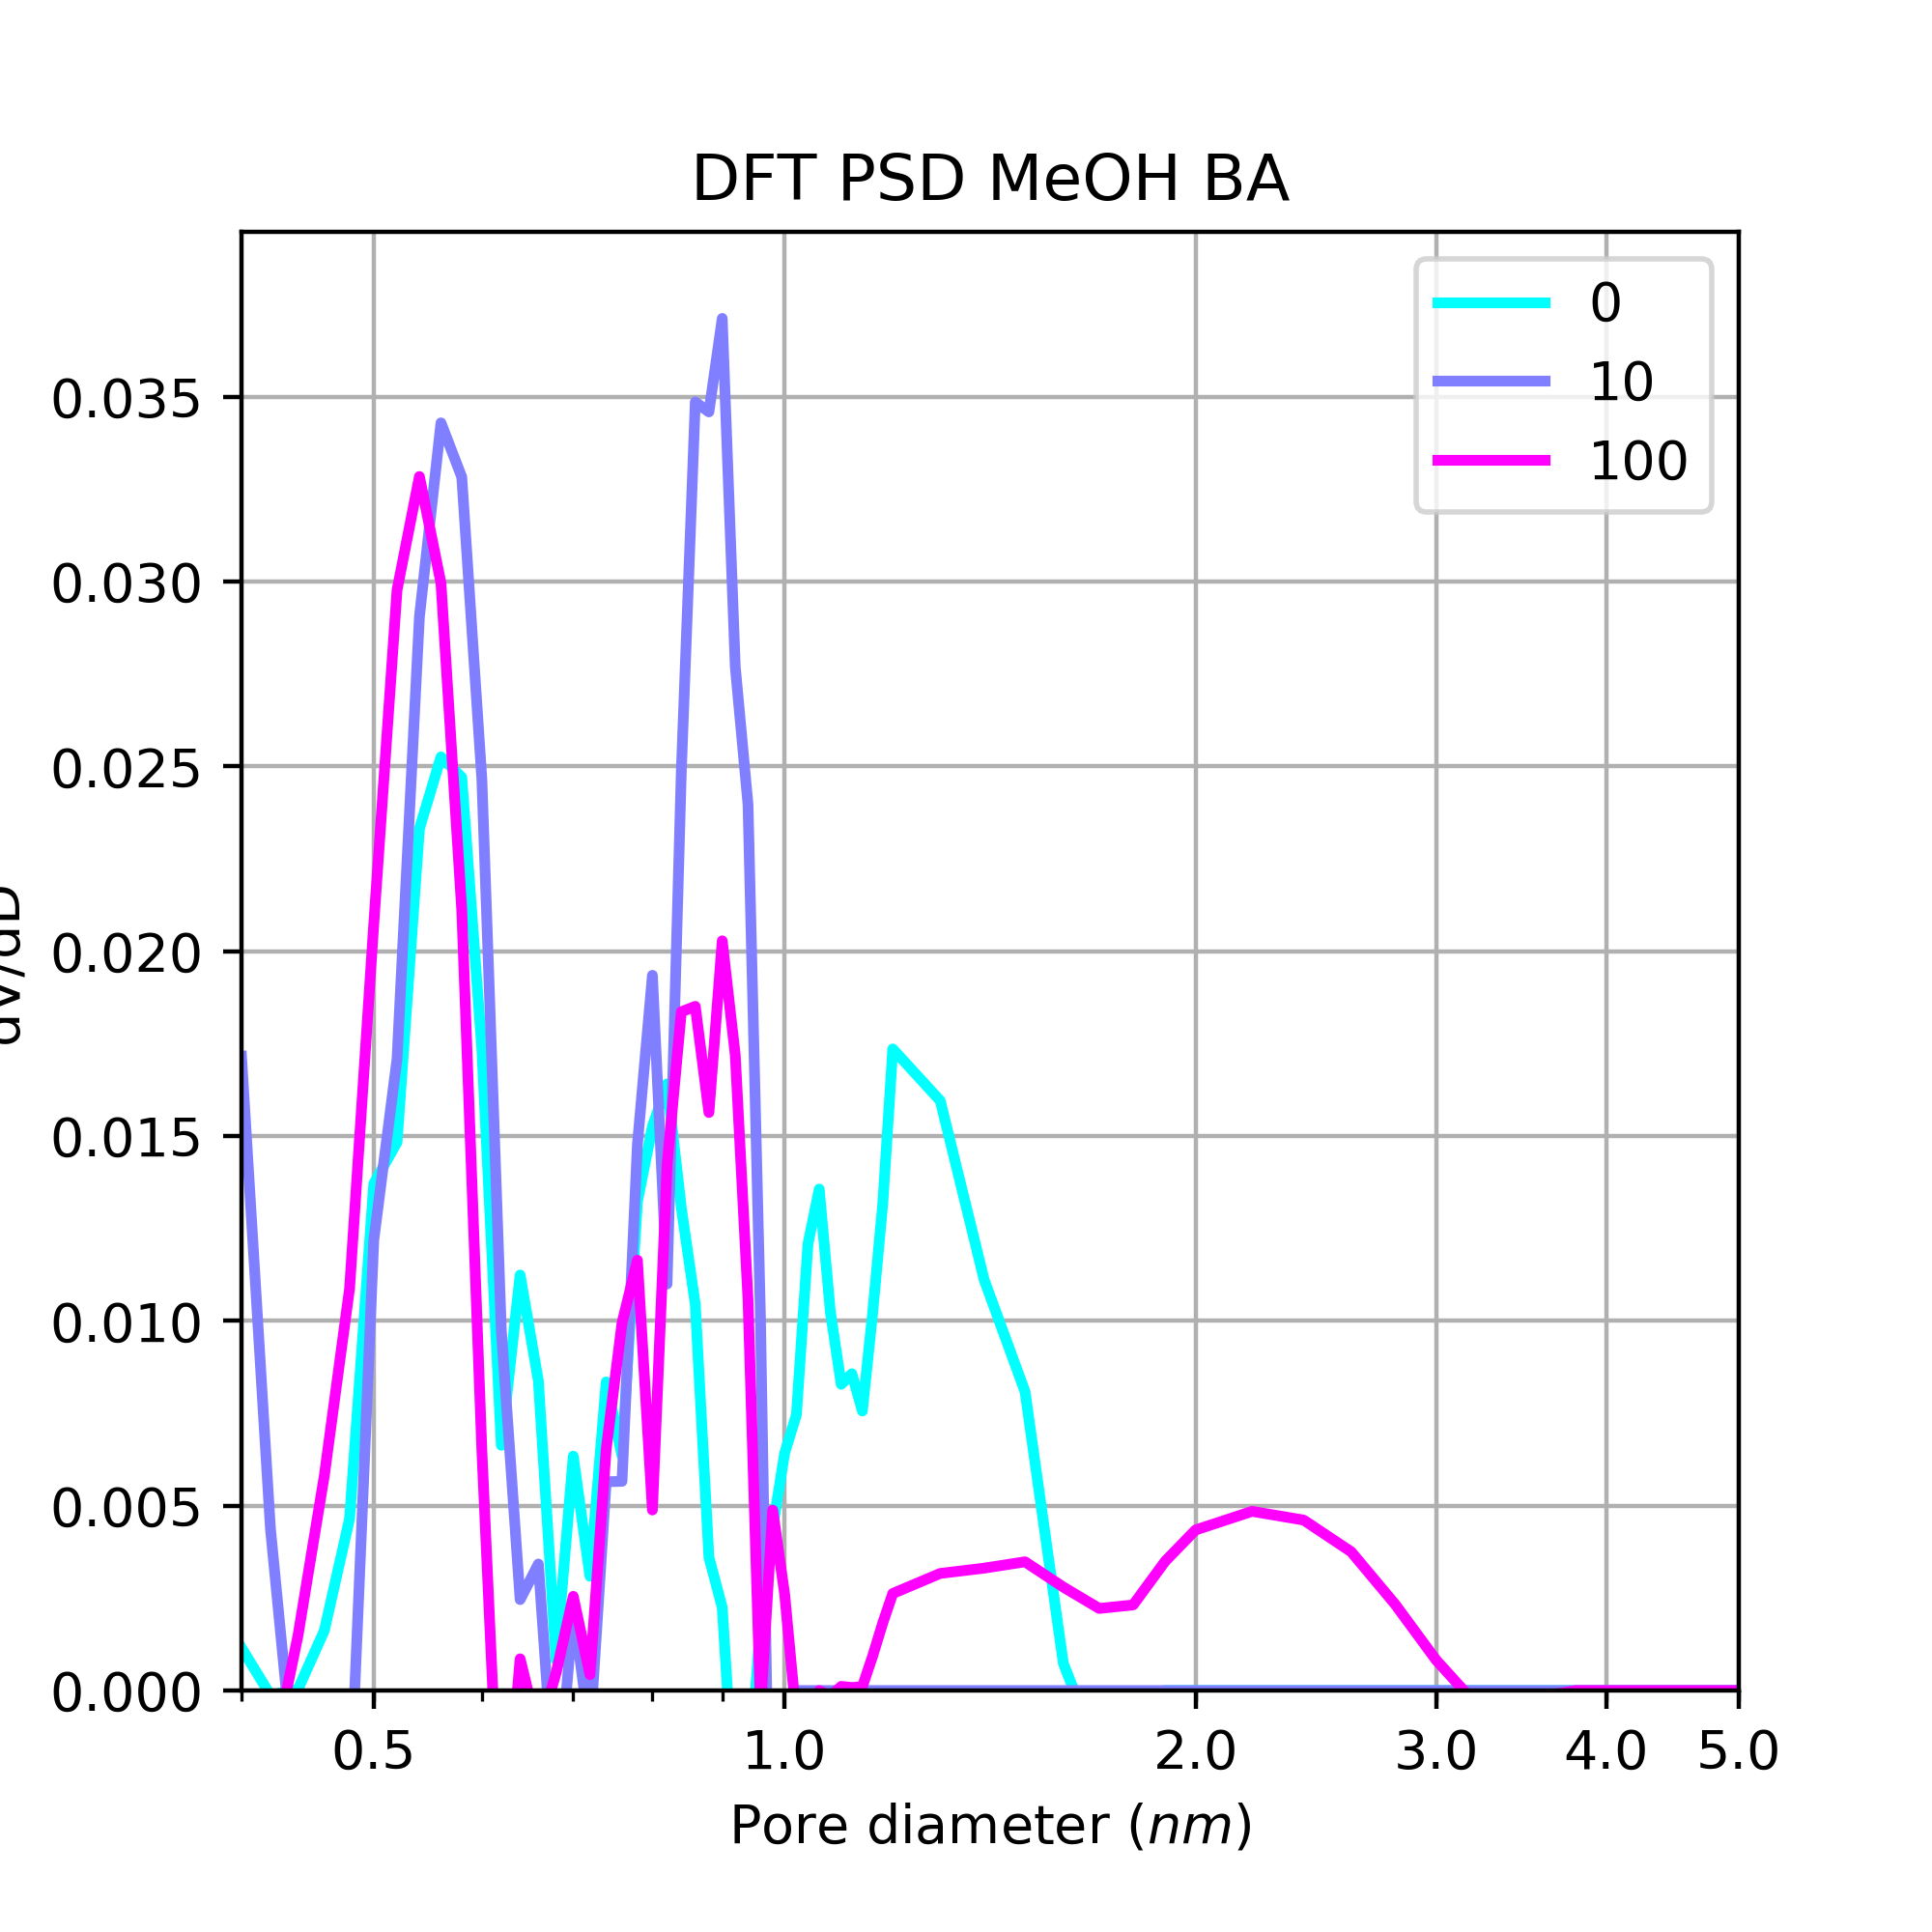
\includegraphics[width=\textwidth]{n2phys/meoh-ba-psd-dft}%
        \label{appx:def:fgr:psd-meoh-ba-dft}
    \end{subfigure}%
    
    \begin{subfigure}{0.25\linewidth}
        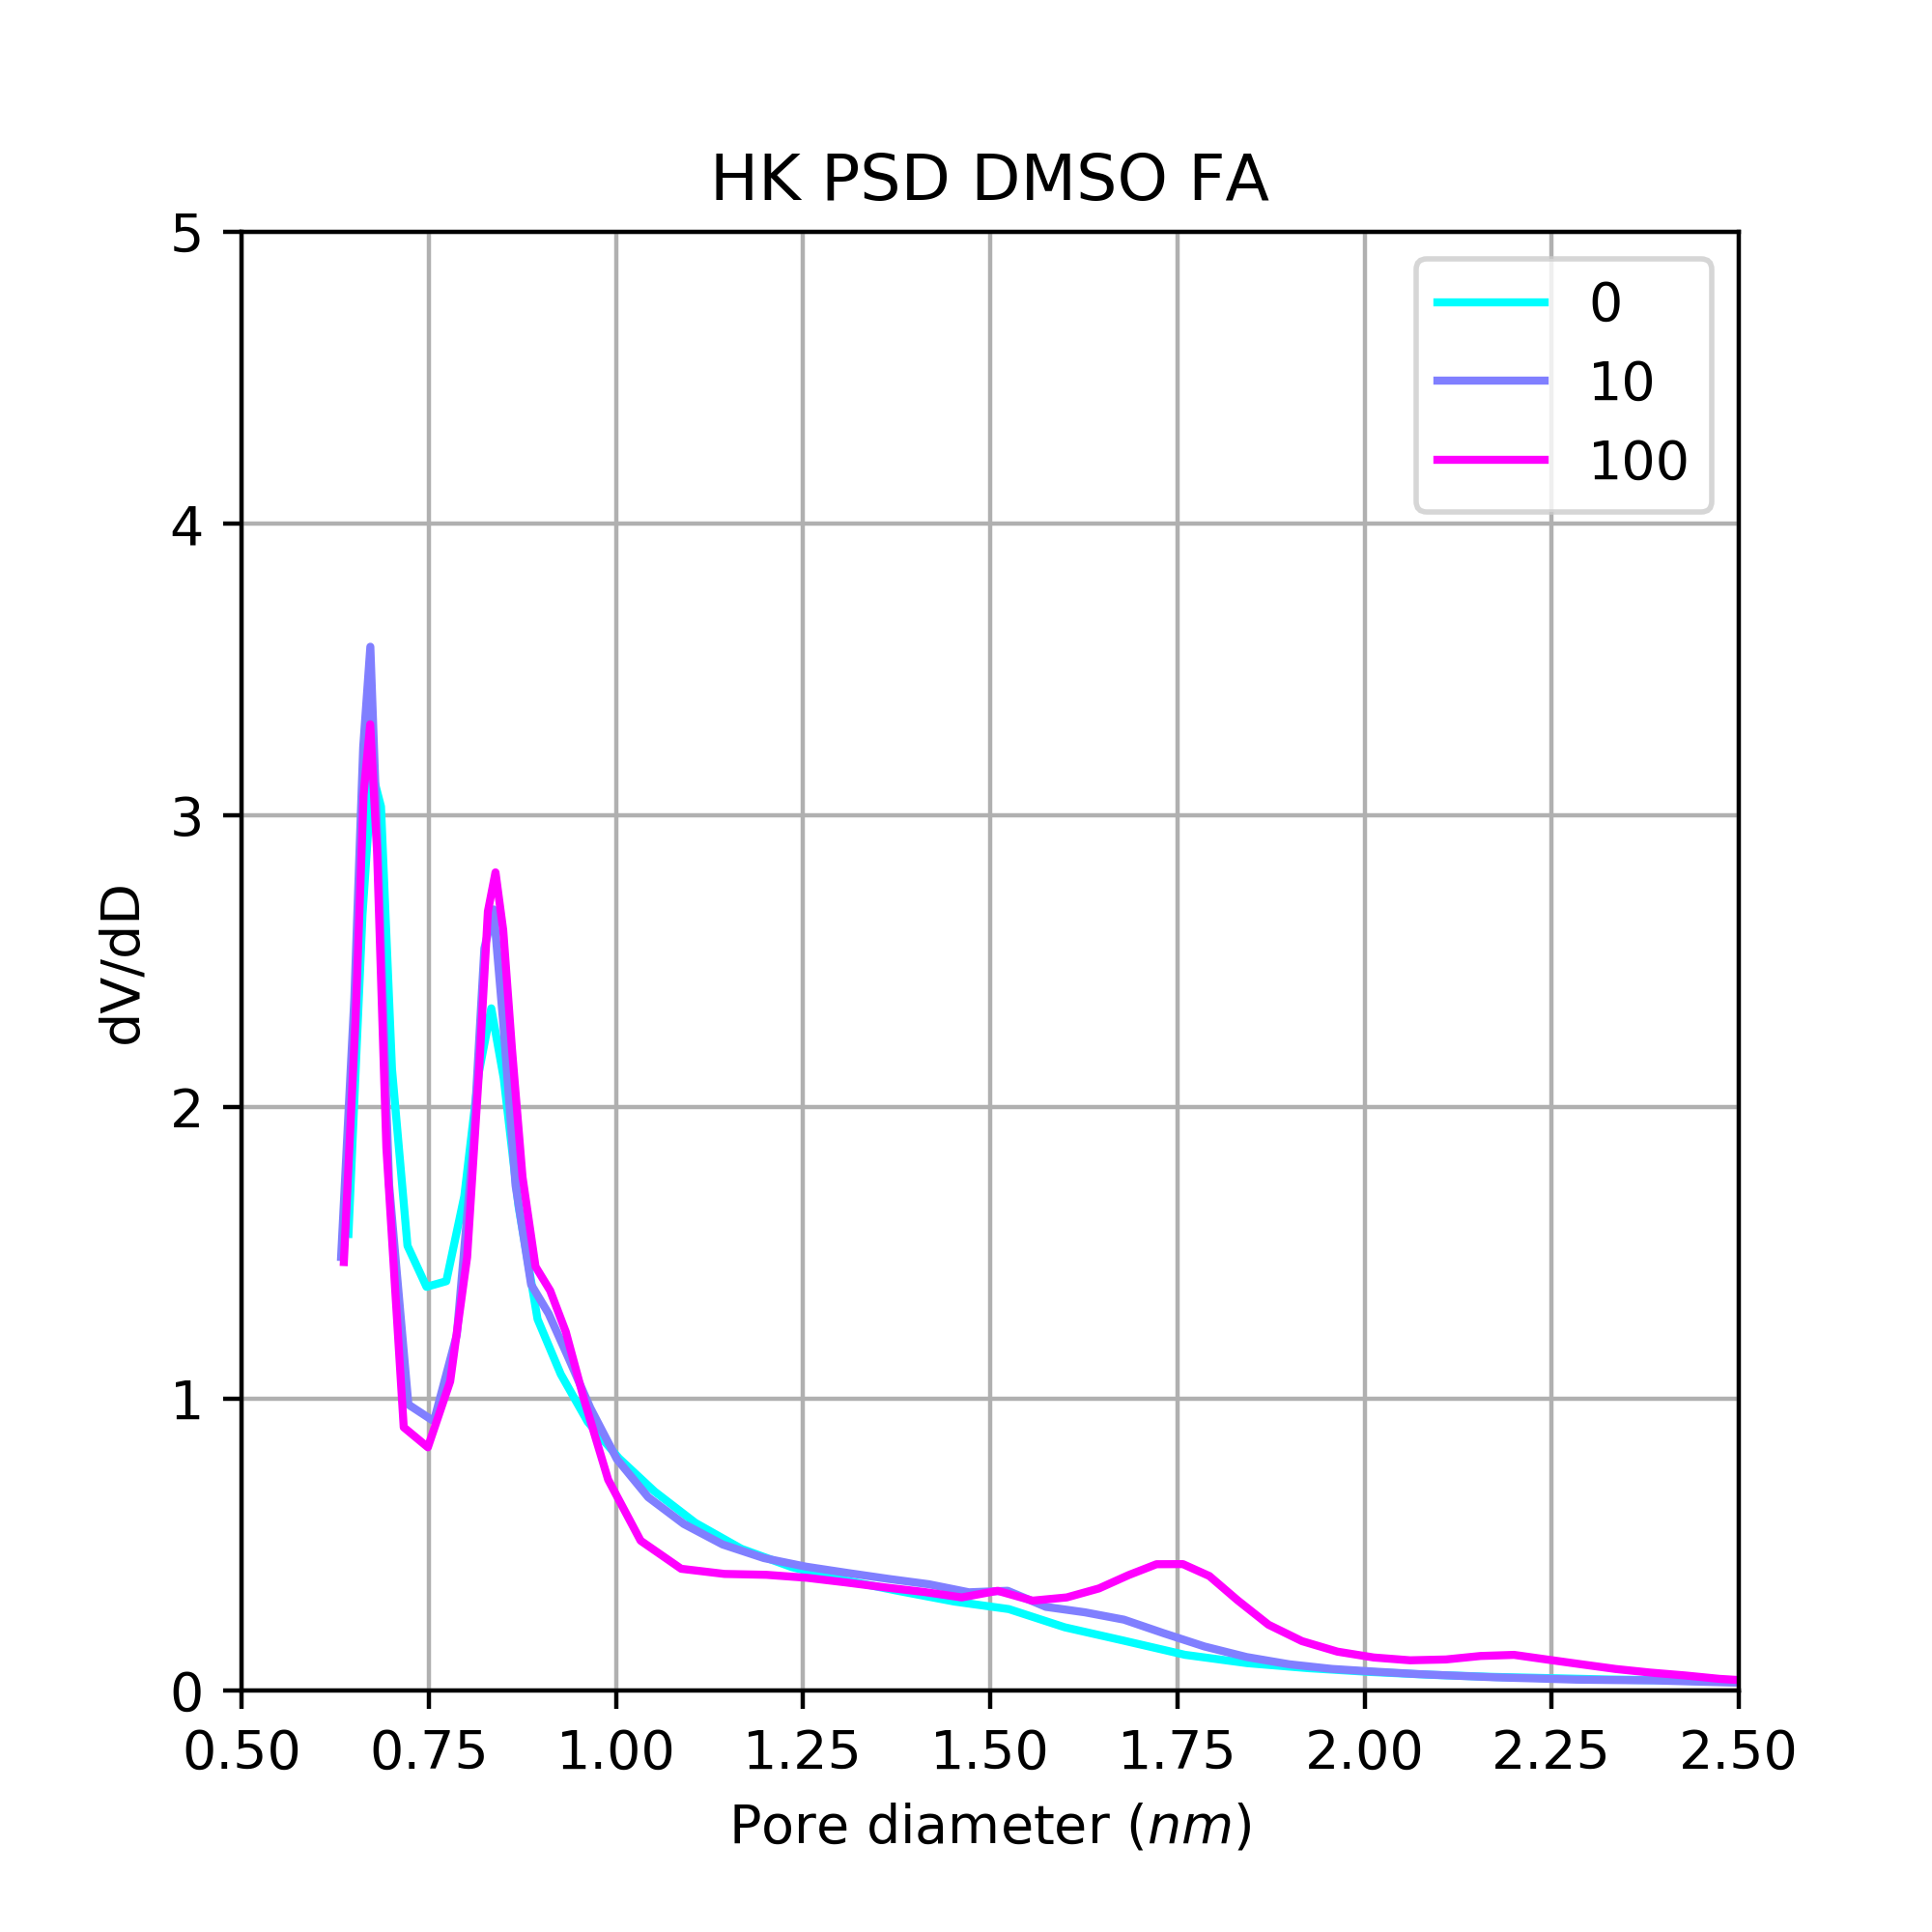
\includegraphics[width=\textwidth]{n2phys/dmso-fa-psd-hk}%
        \label{appx:def:fgr:psd-dmso-fa-hk}
    \end{subfigure}%
    \begin{subfigure}{0.25\linewidth}
        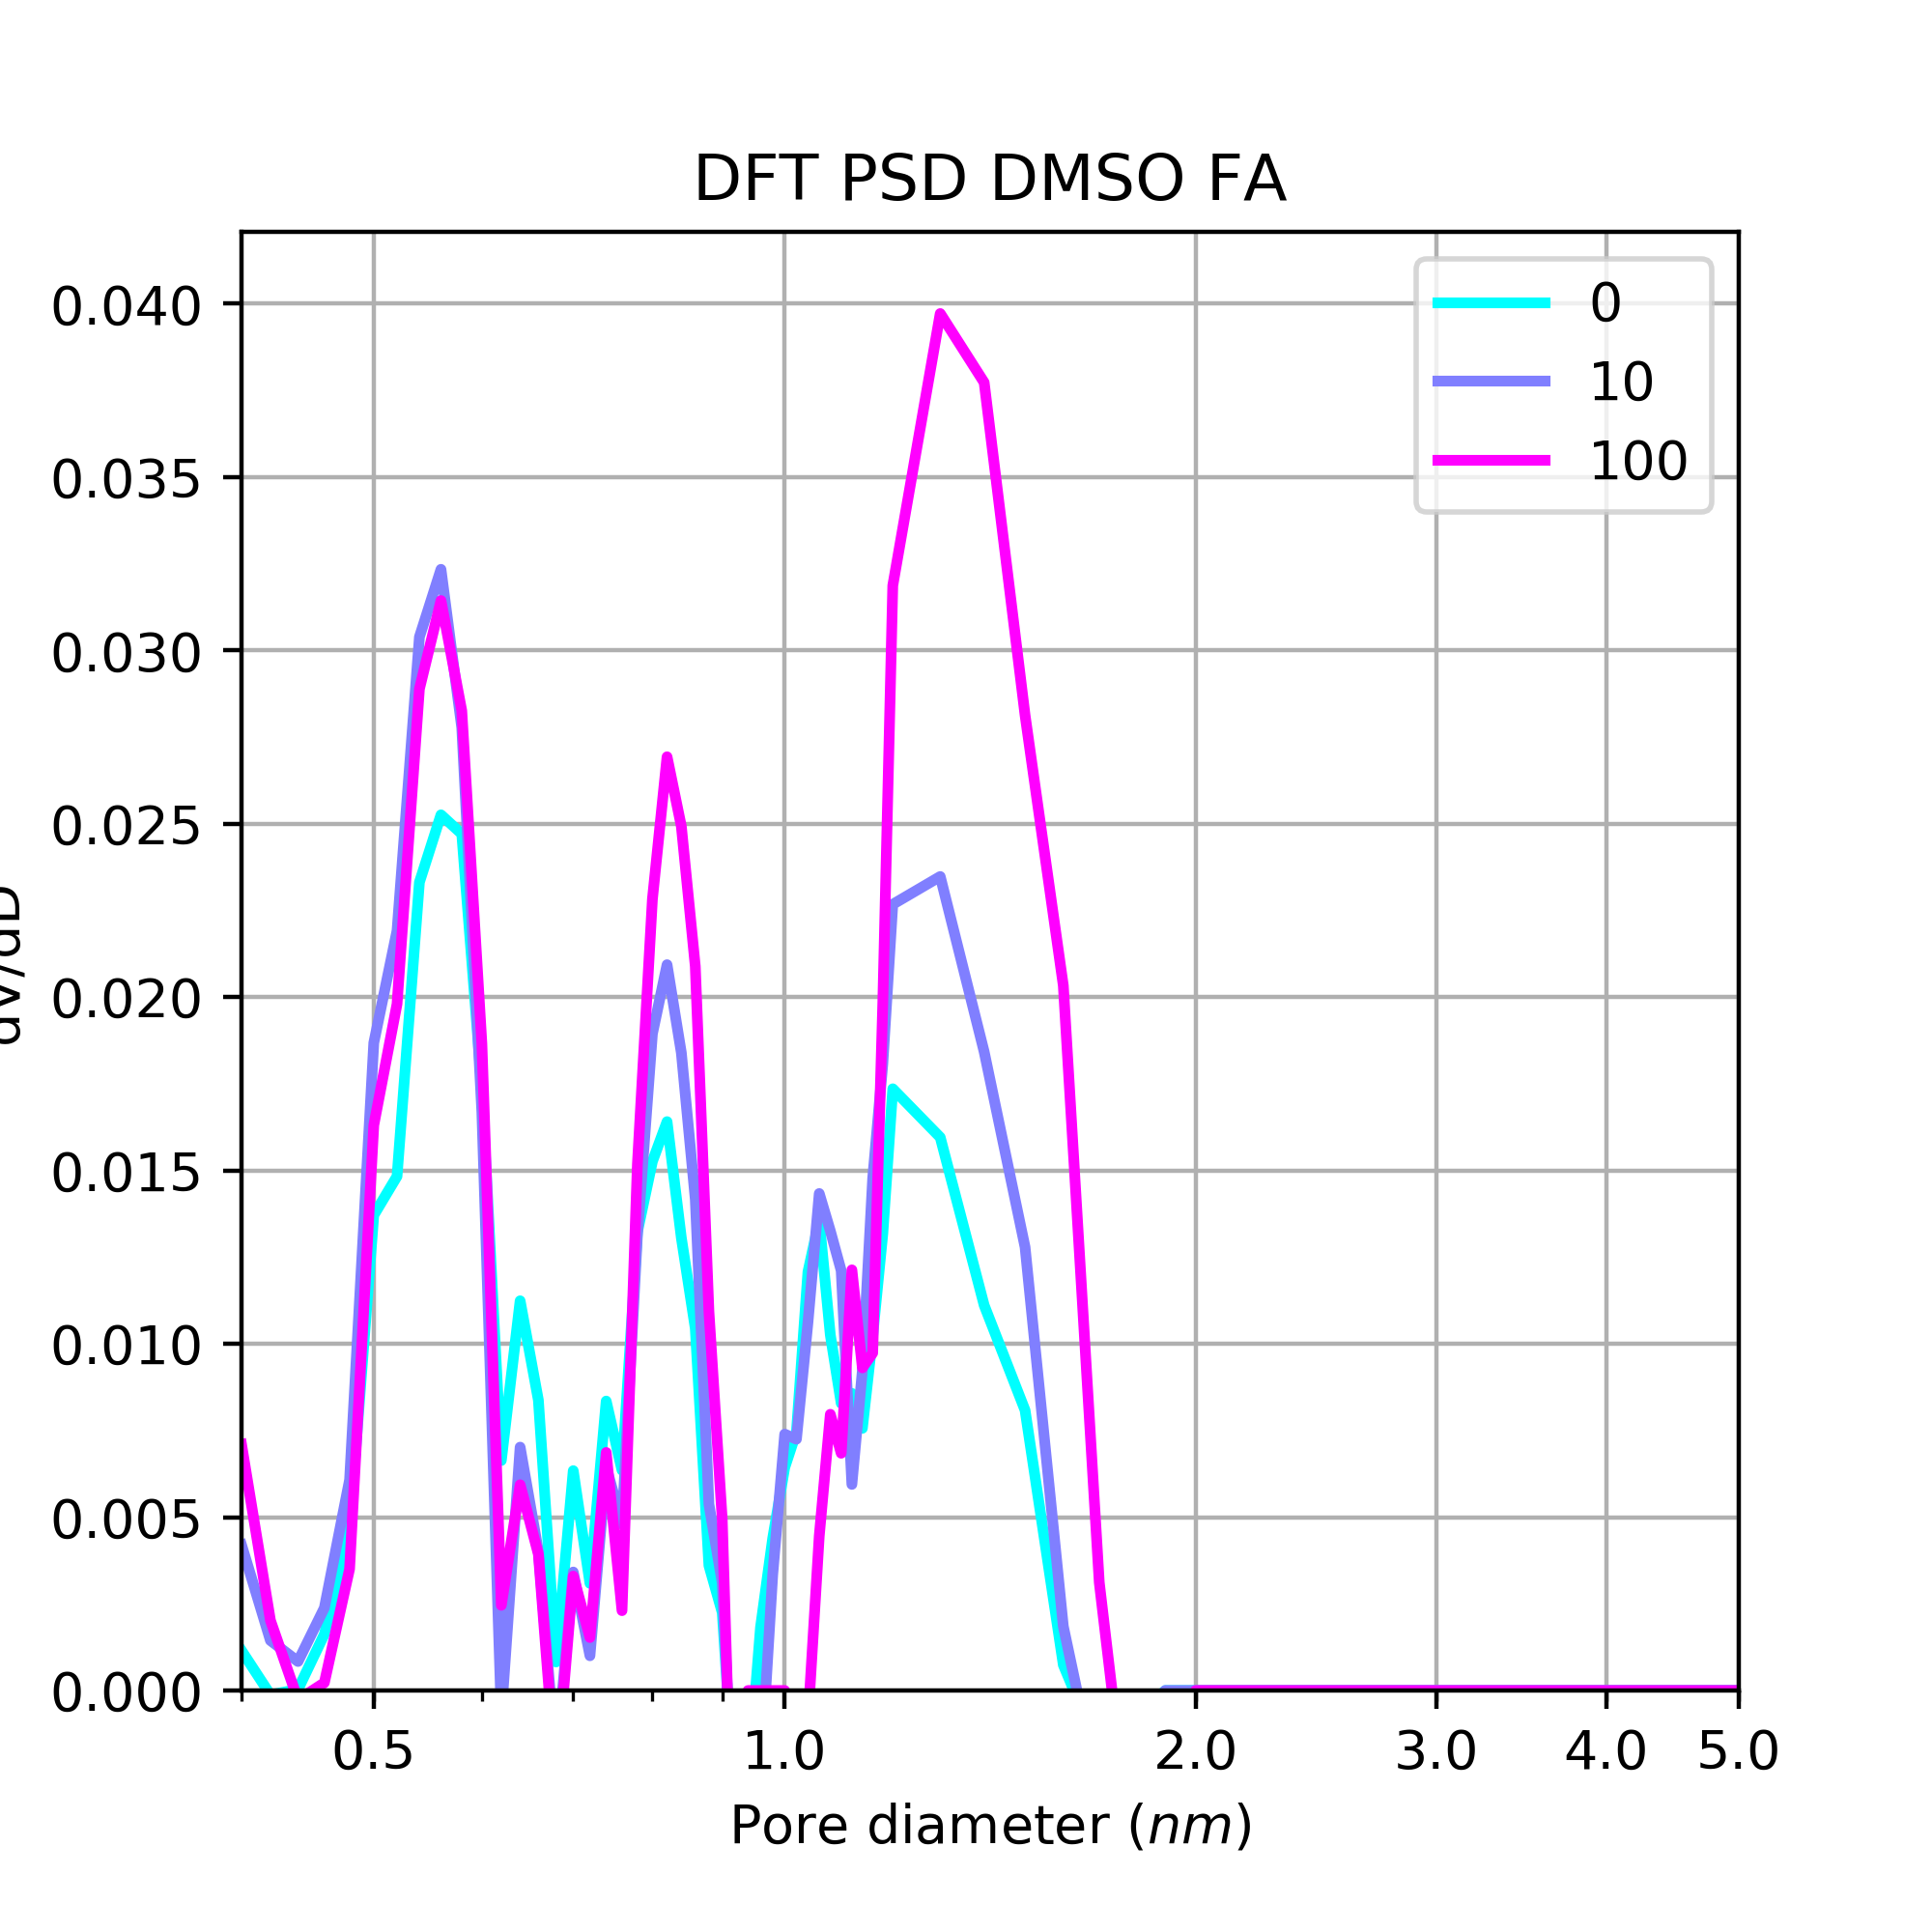
\includegraphics[width=\textwidth]{n2phys/dmso-fa-psd-dft}%
        \label{appx:def:fgr:psd-dmso-fa-dft}
    \end{subfigure}%
    \begin{subfigure}{0.25\linewidth}
        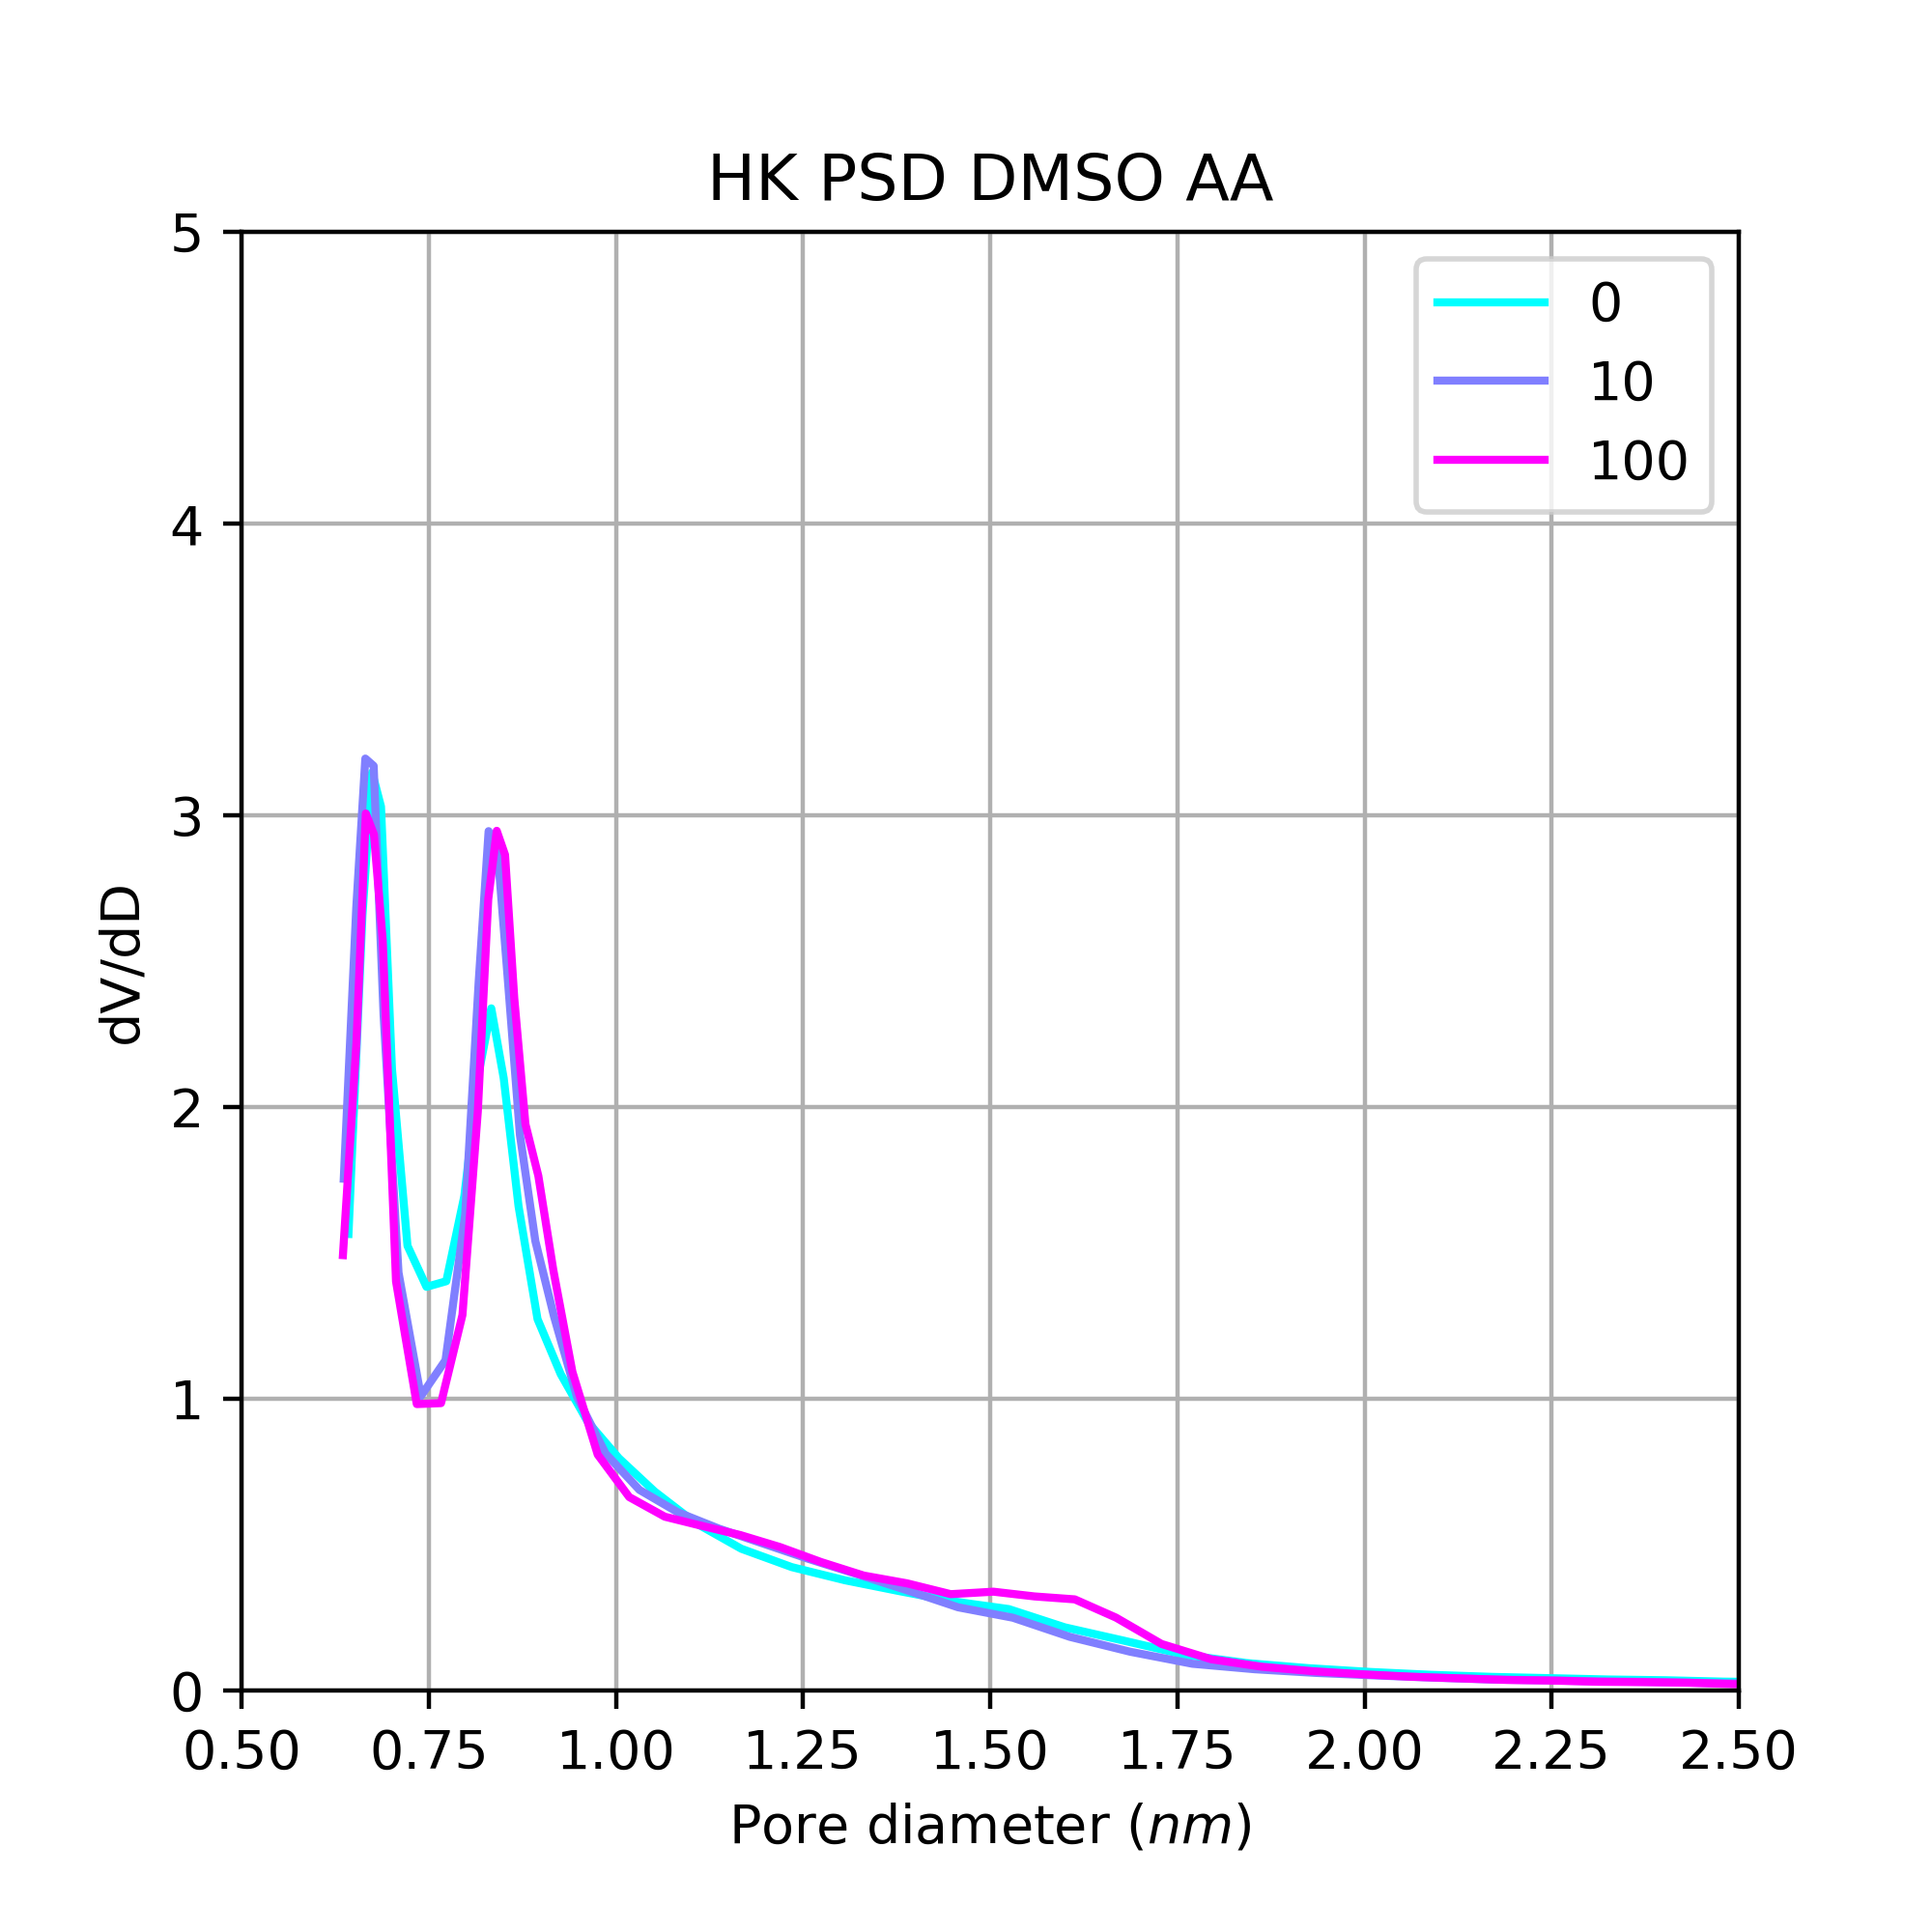
\includegraphics[width=\textwidth]{n2phys/dmso-aa-psd-hk}%
        \label{appx:def:fgr:psd-dmso-aa-hk}
    \end{subfigure}%
    \begin{subfigure}{0.25\linewidth}
        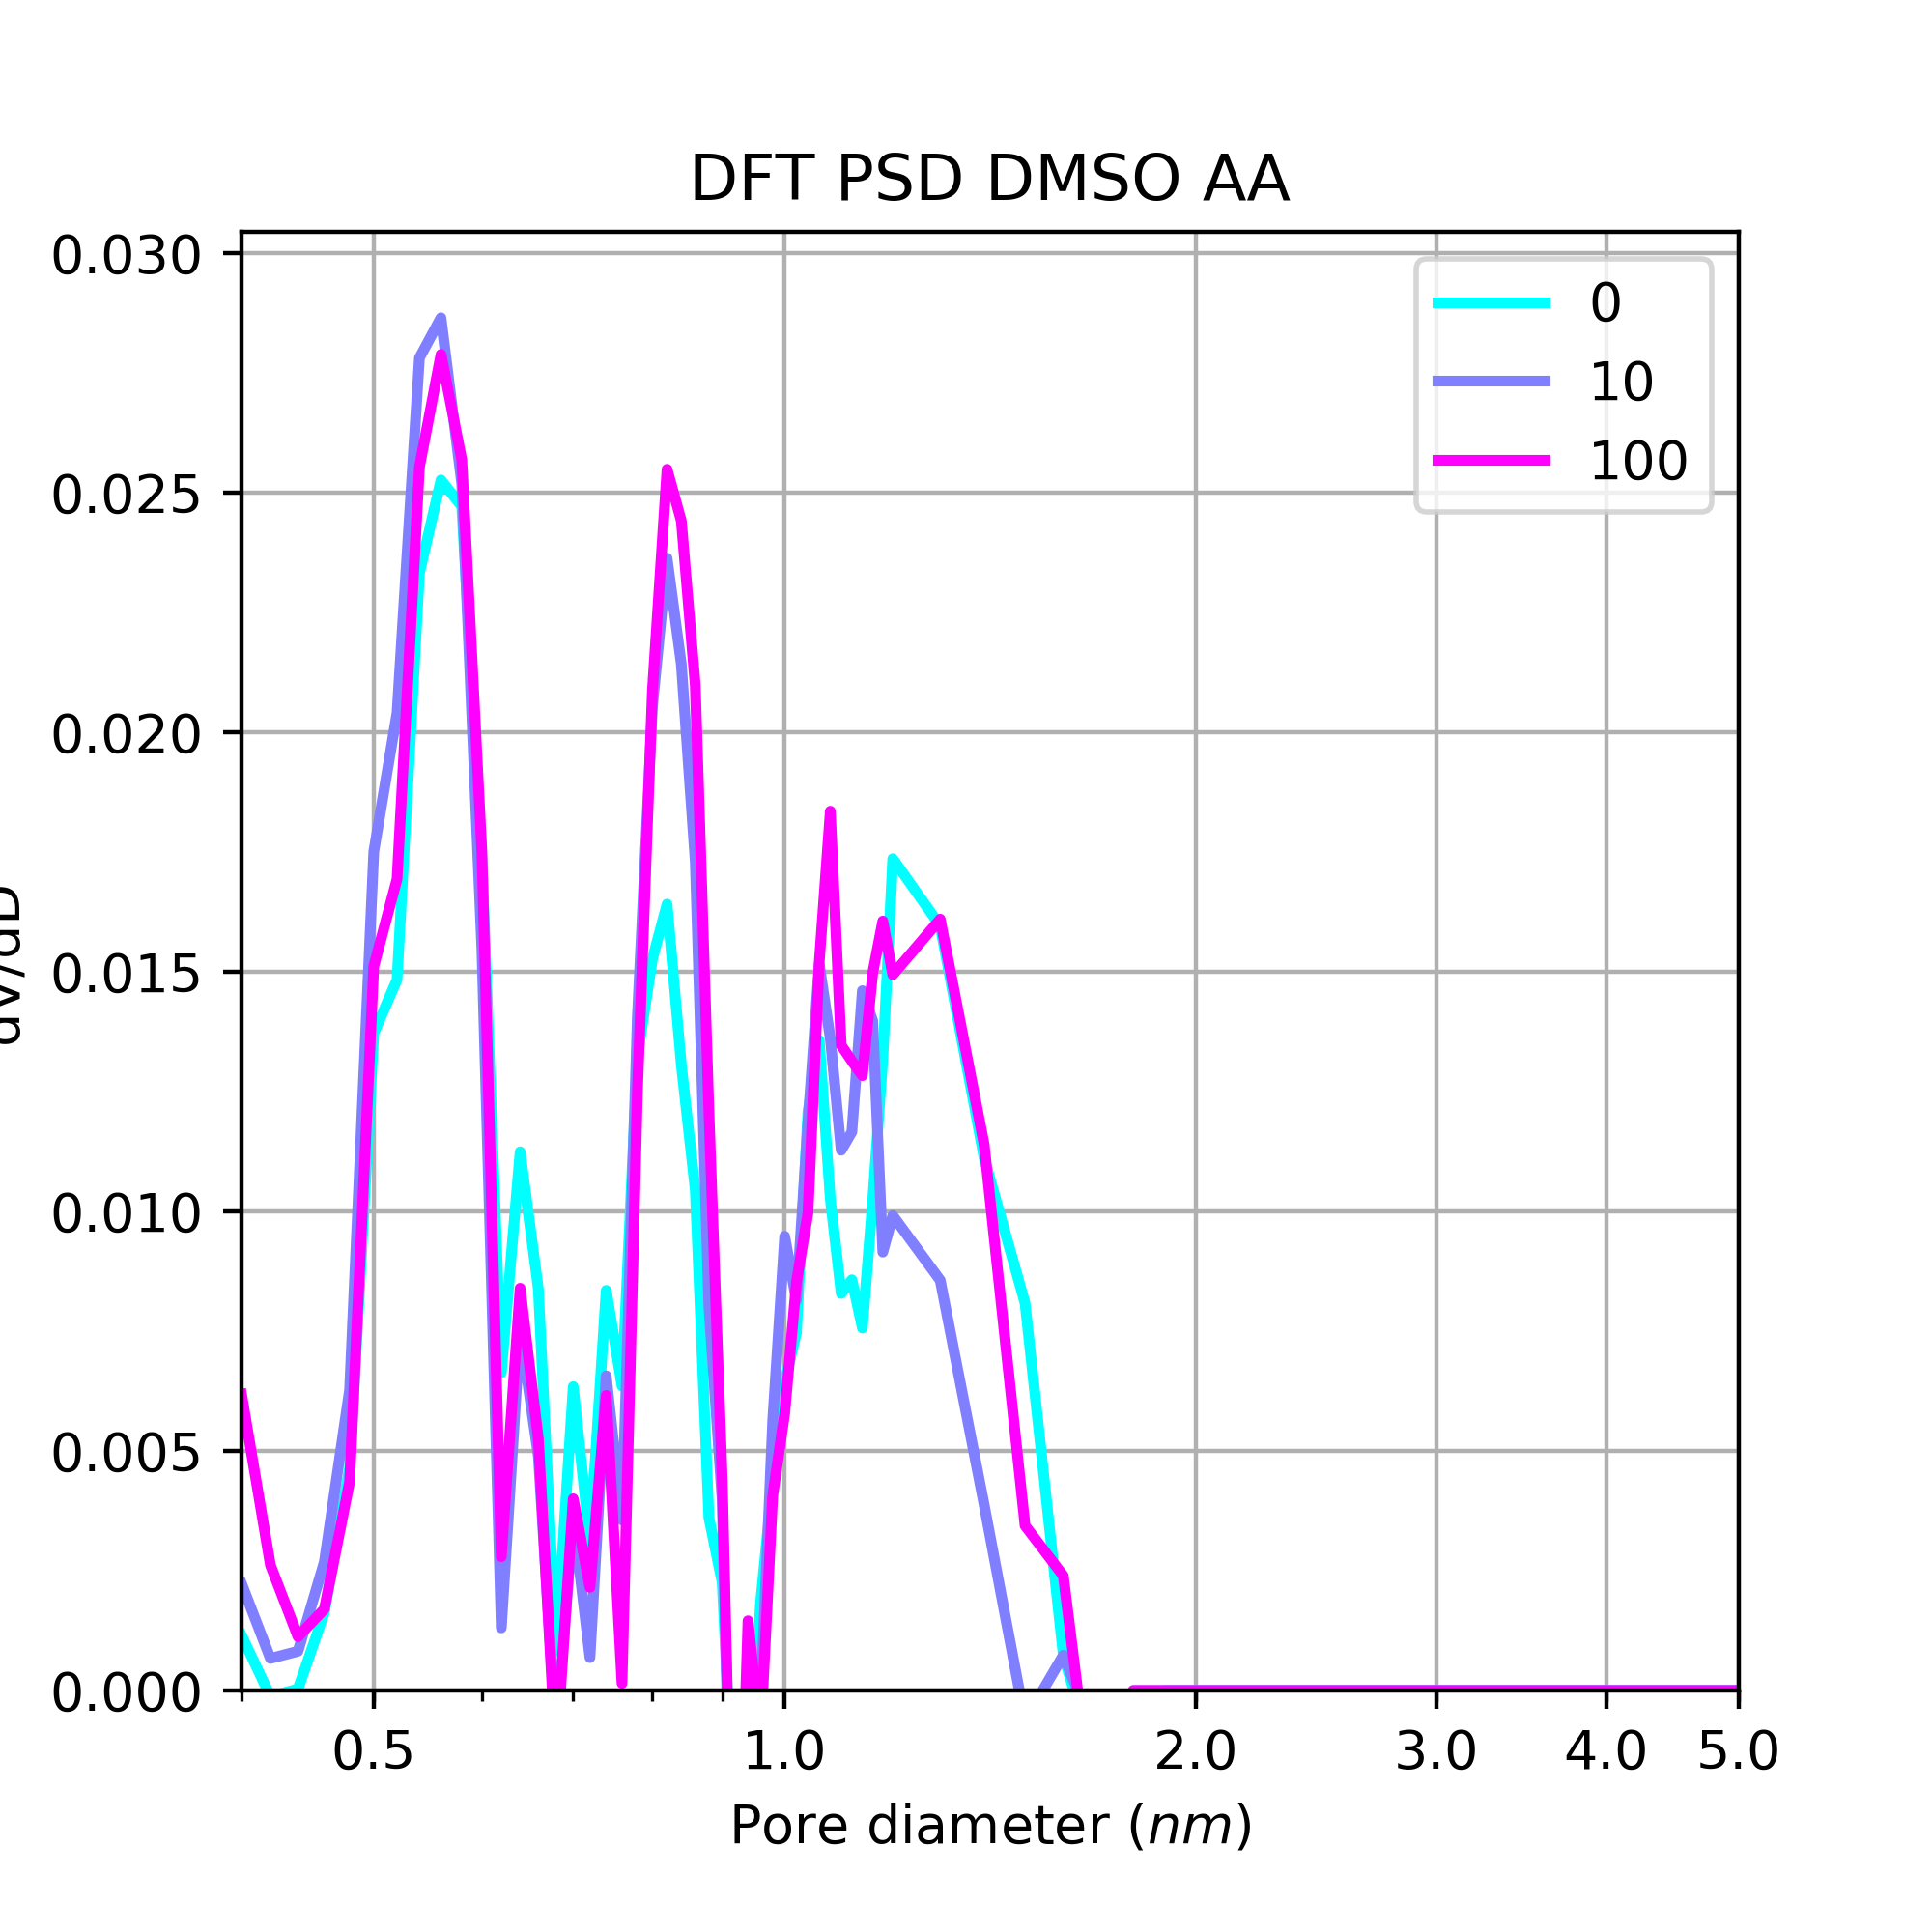
\includegraphics[width=\textwidth]{n2phys/dmso-aa-psd-dft}%
        \label{appx:def:fgr:psd-dmso-aa-dft}
    \end{subfigure}%

    \begin{subfigure}{0.25\linewidth}
        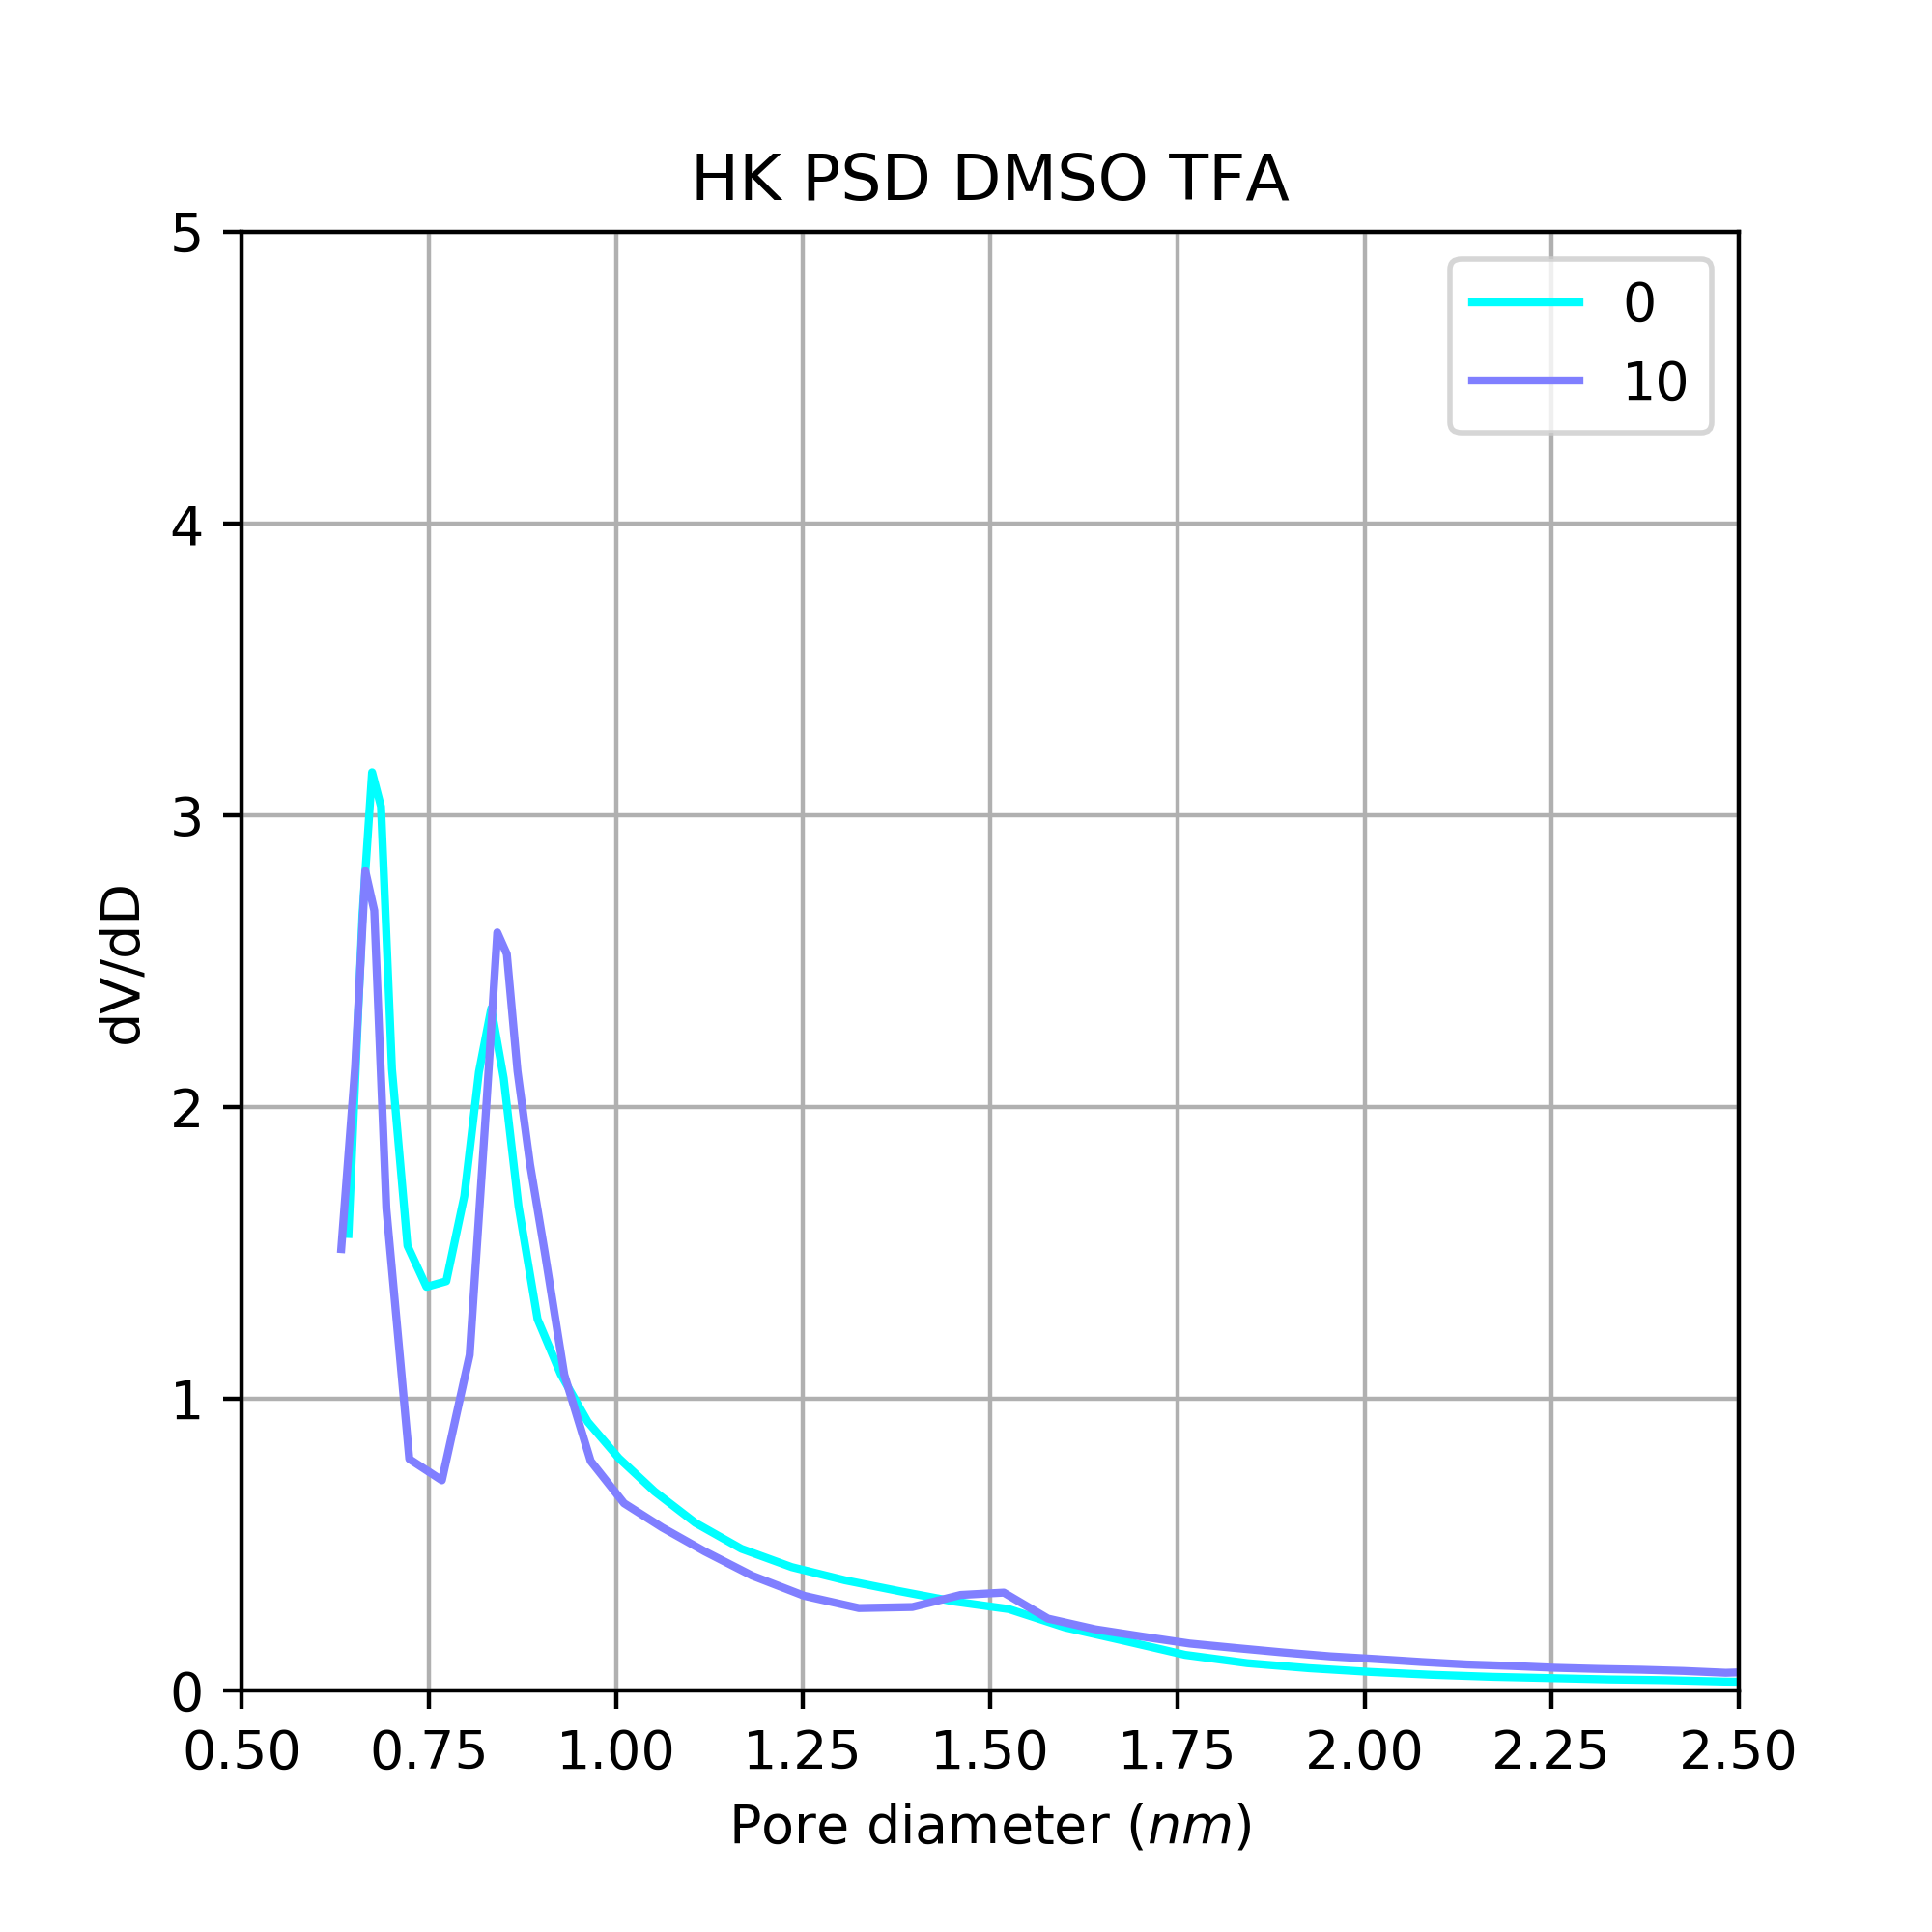
\includegraphics[width=\textwidth]{n2phys/dmso-tfa-psd-hk}%
        \label{appx:def:fgr:psd-dmso-tfa-hk}
    \end{subfigure}%
    \begin{subfigure}{0.25\linewidth}
        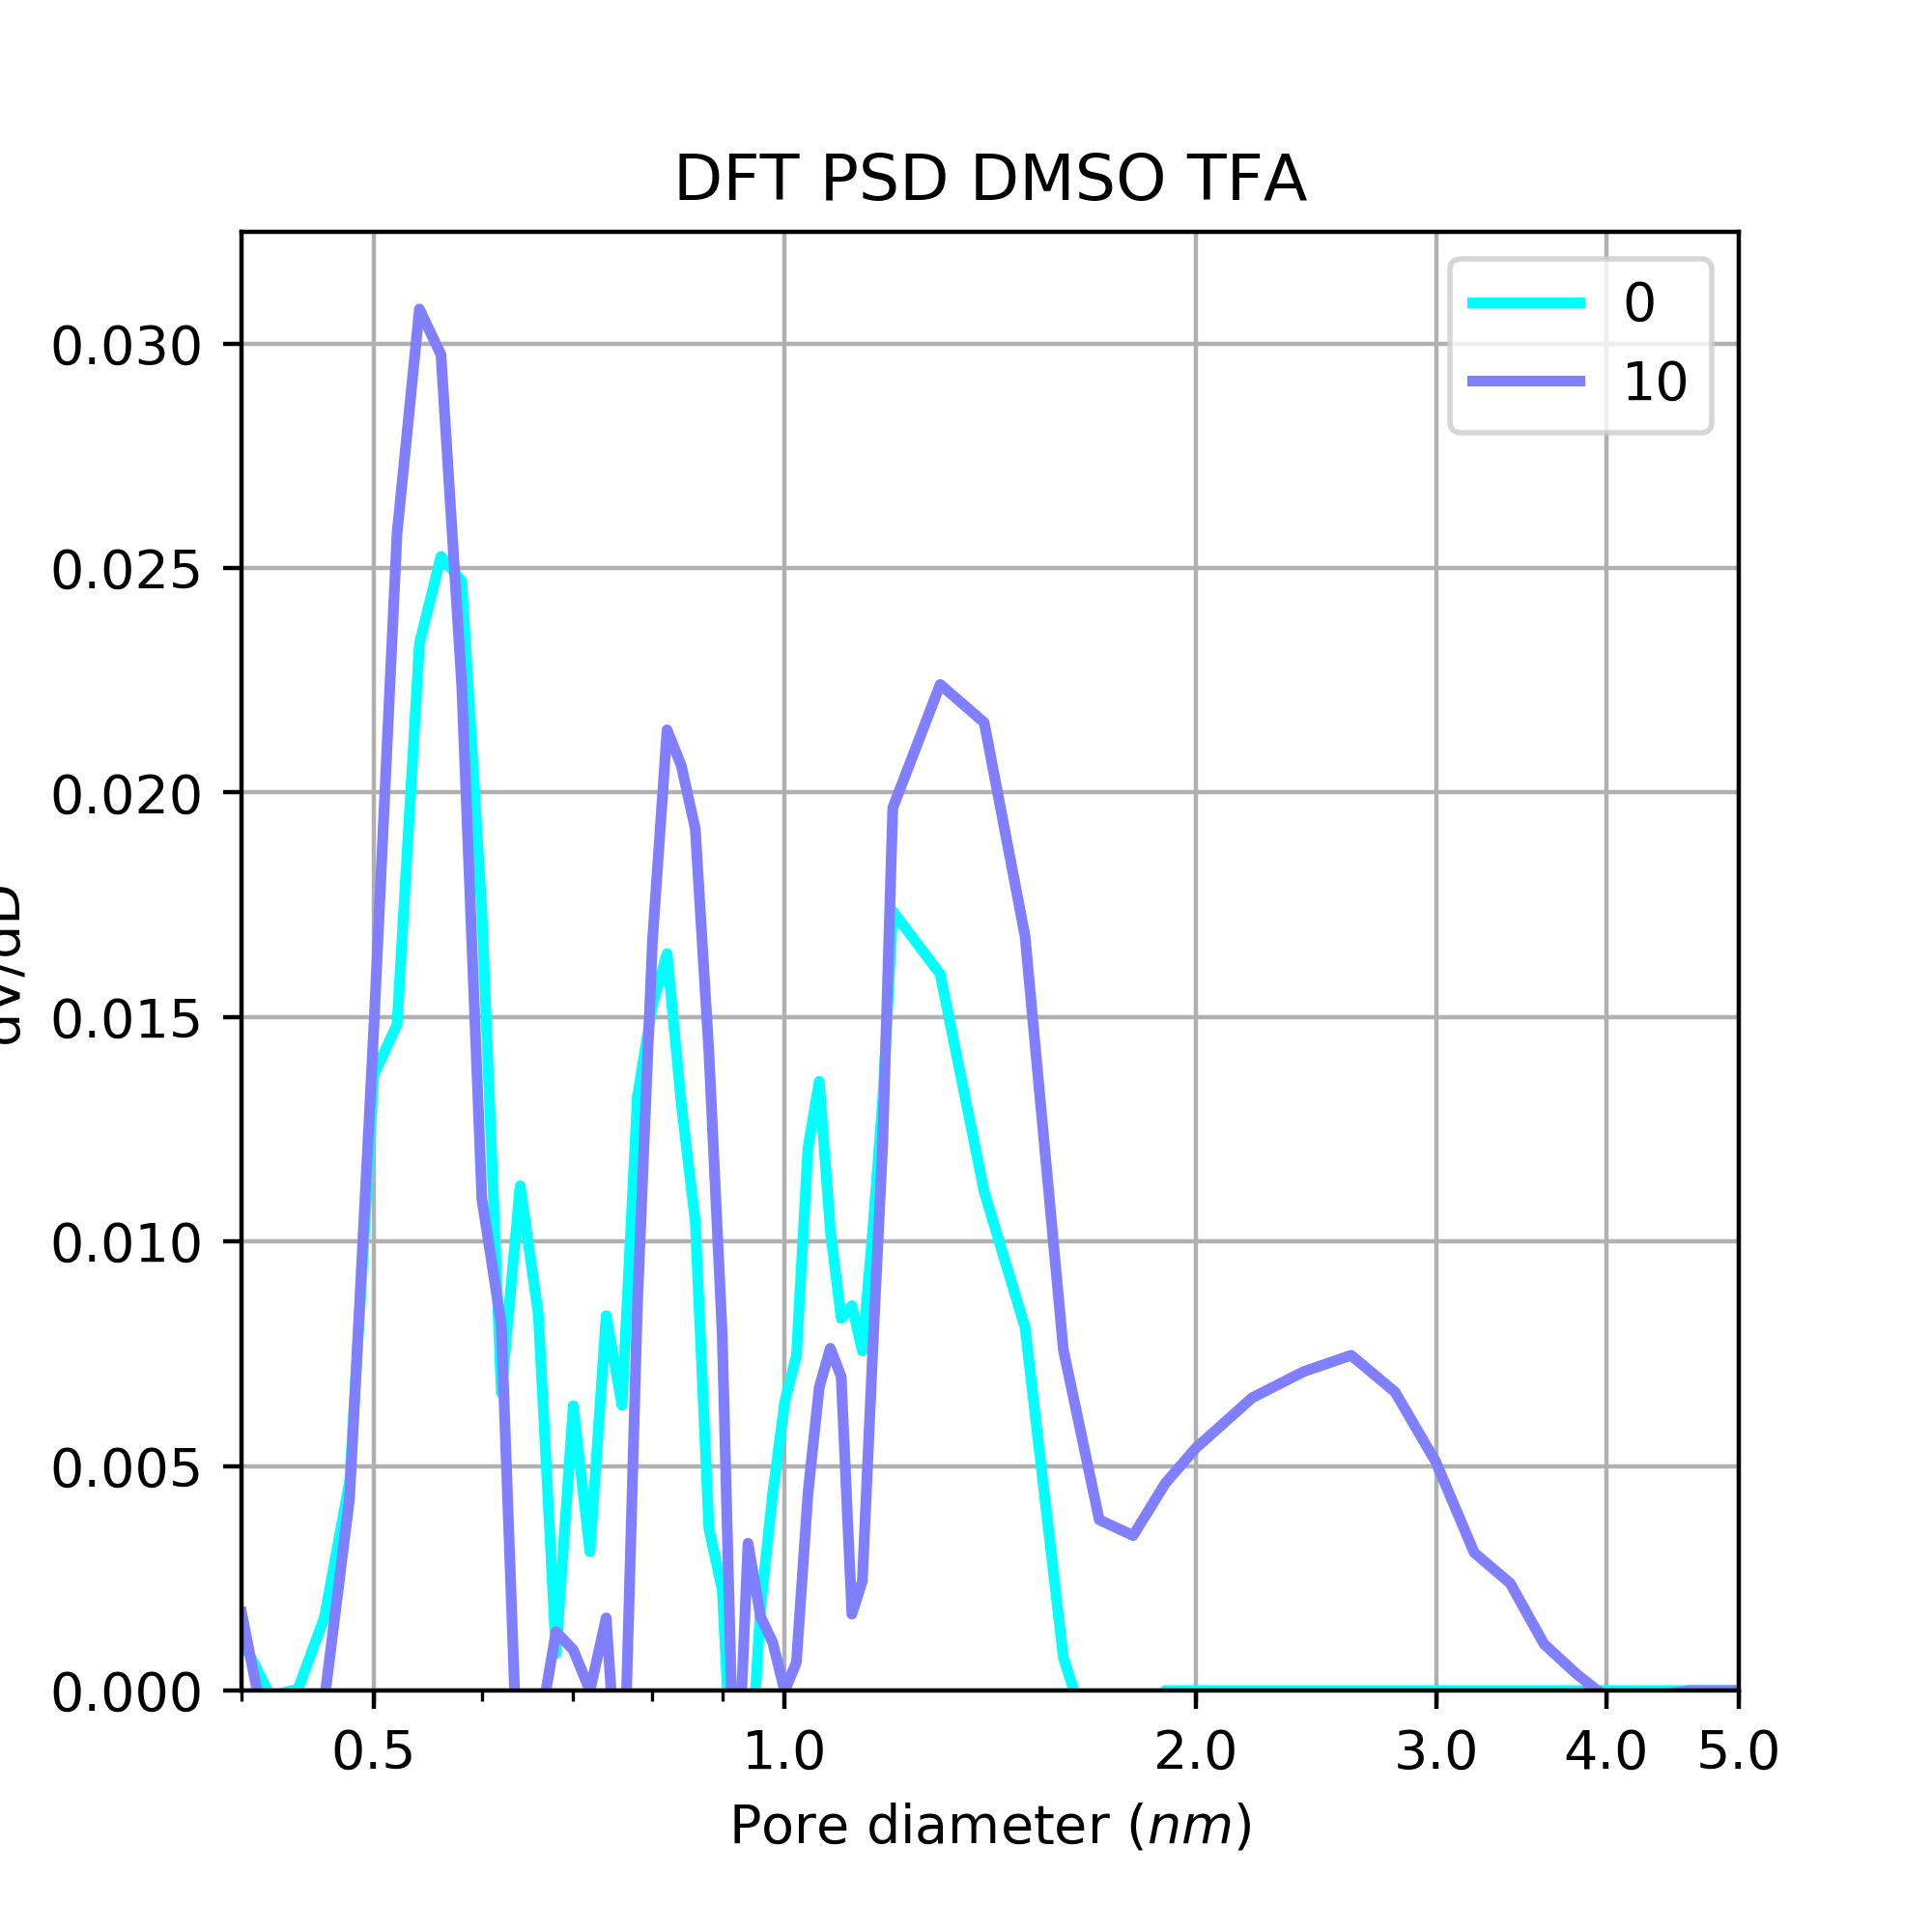
\includegraphics[width=\textwidth]{n2phys/dmso-tfa-psd-dft}%
        \label{appx:def:fgr:psd-dmso-tfa-dft}
    \end{subfigure}%
    \begin{subfigure}{0.25\linewidth}
        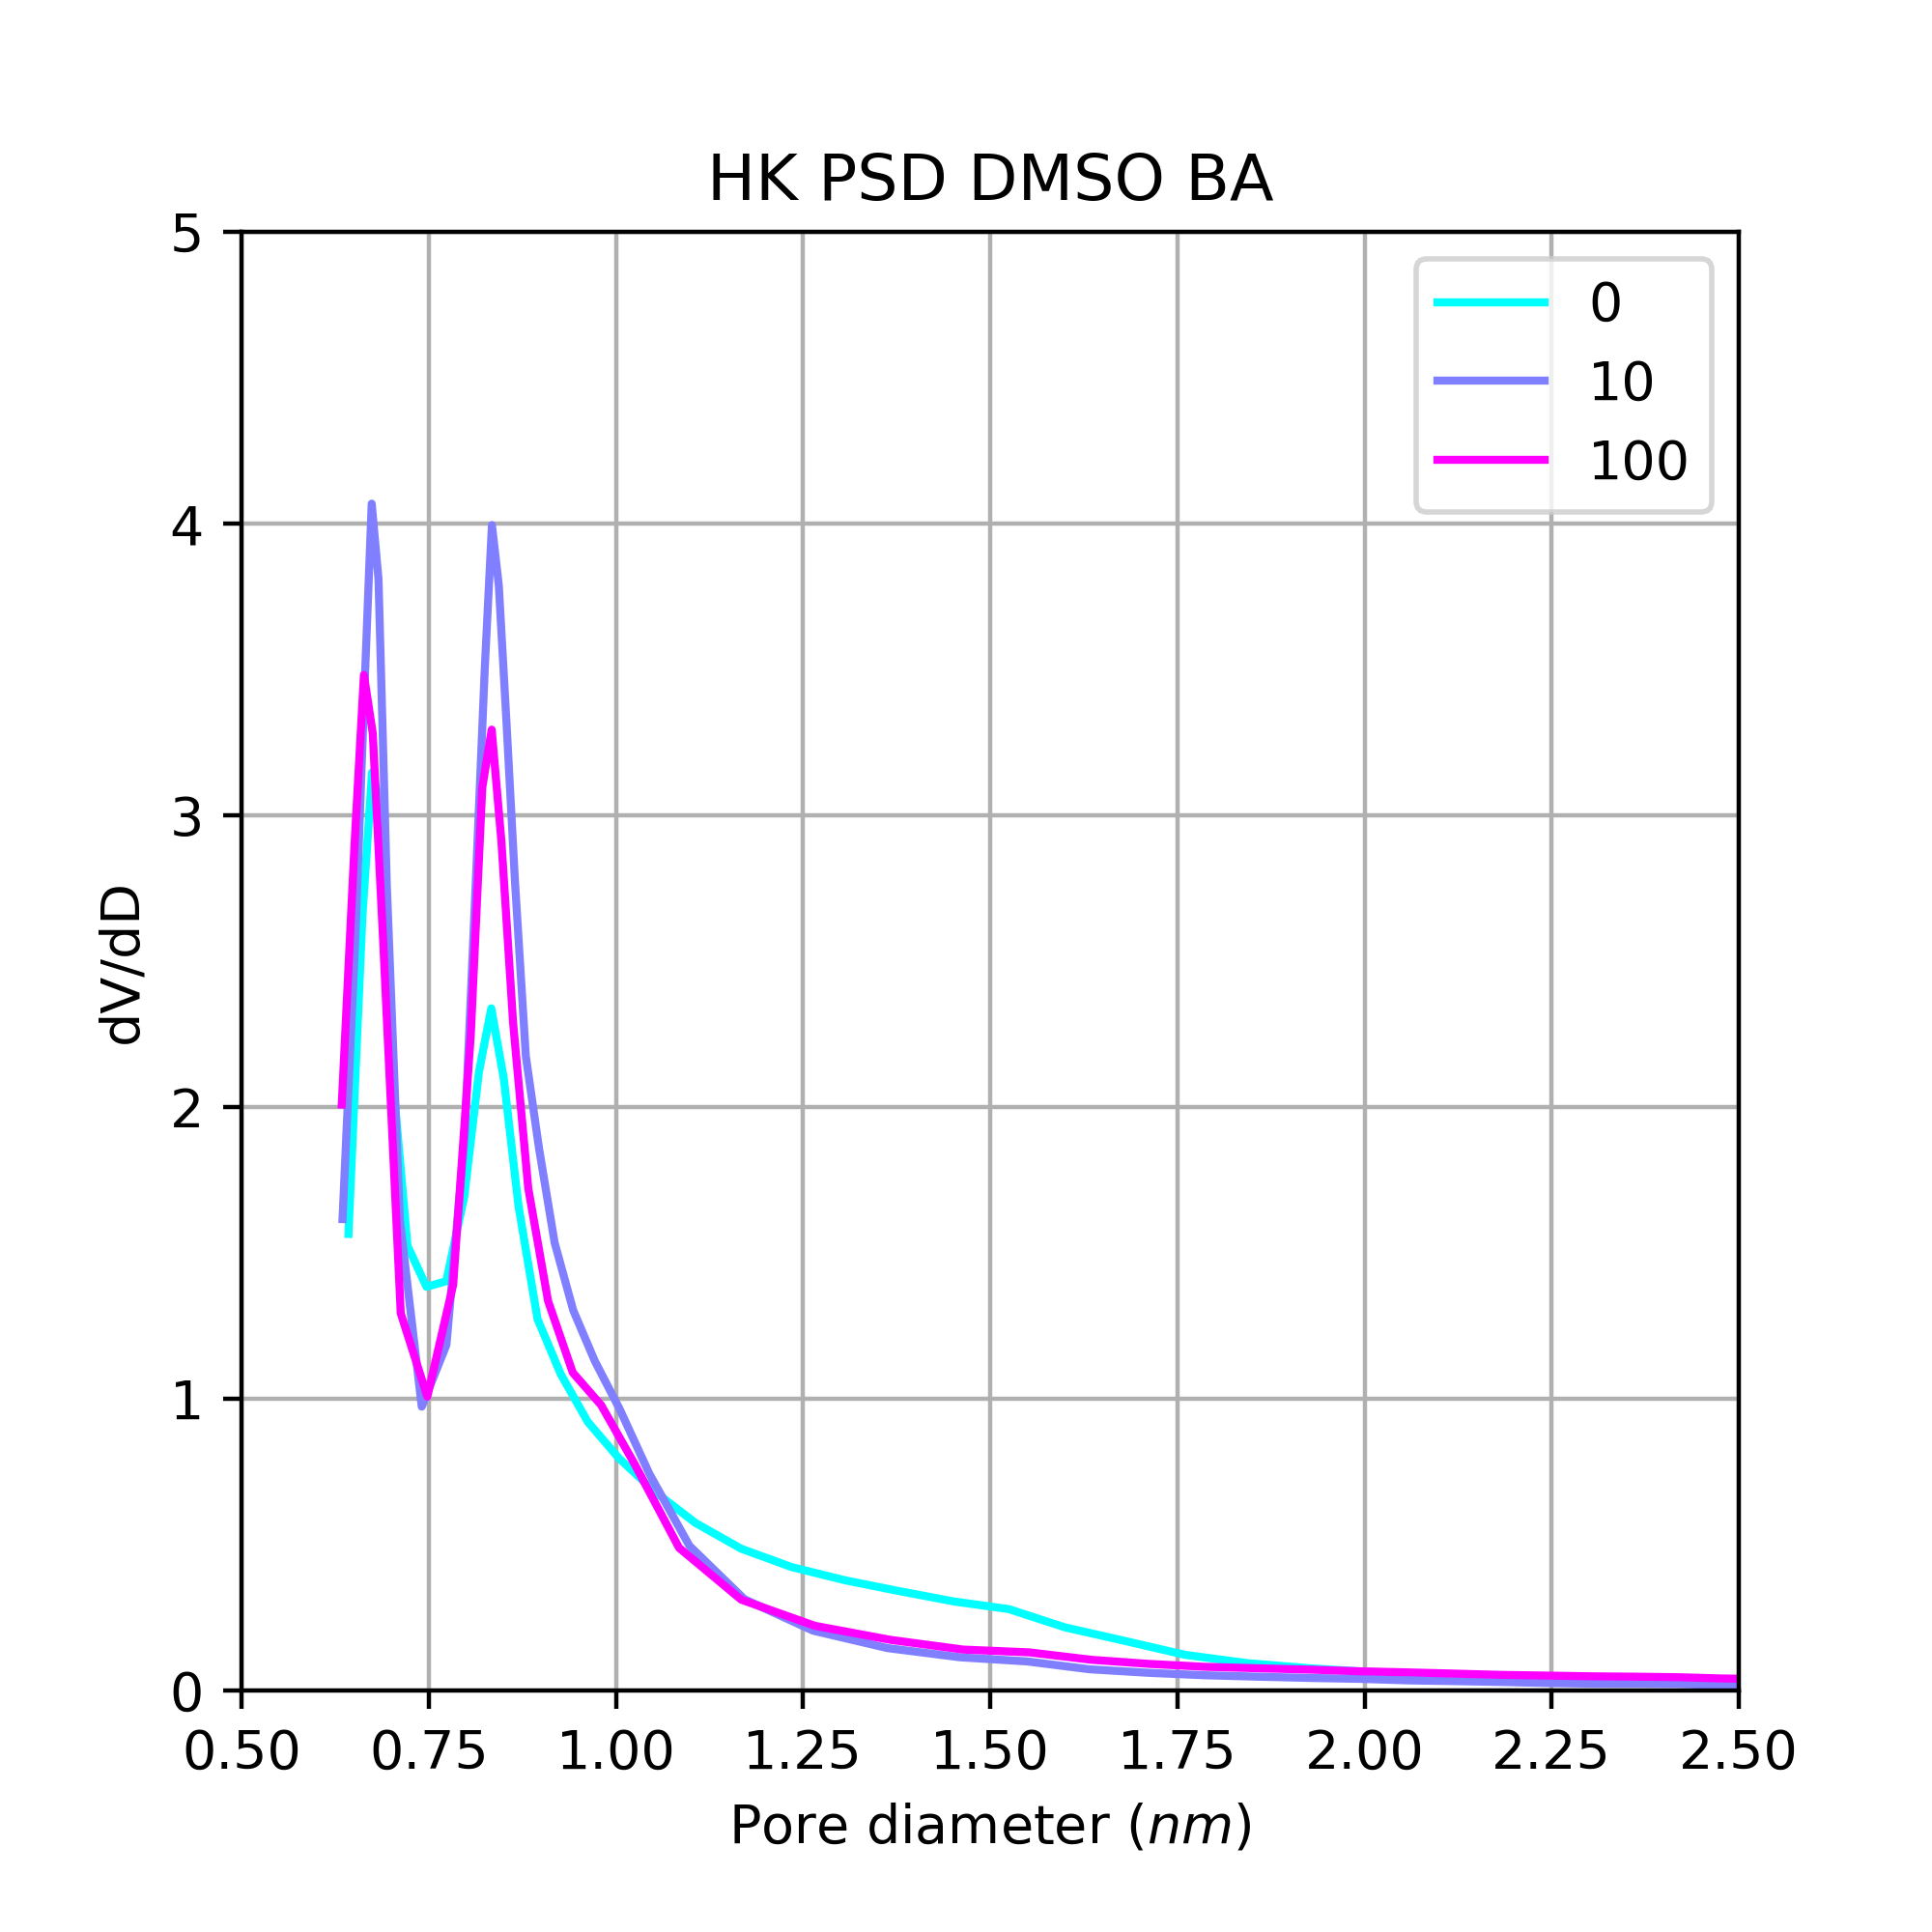
\includegraphics[width=\textwidth]{n2phys/dmso-ba-psd-hk}%
        \label{appx:def:fgr:psd-dmso-ba-hk}
    \end{subfigure}%
    \begin{subfigure}{0.25\linewidth}
        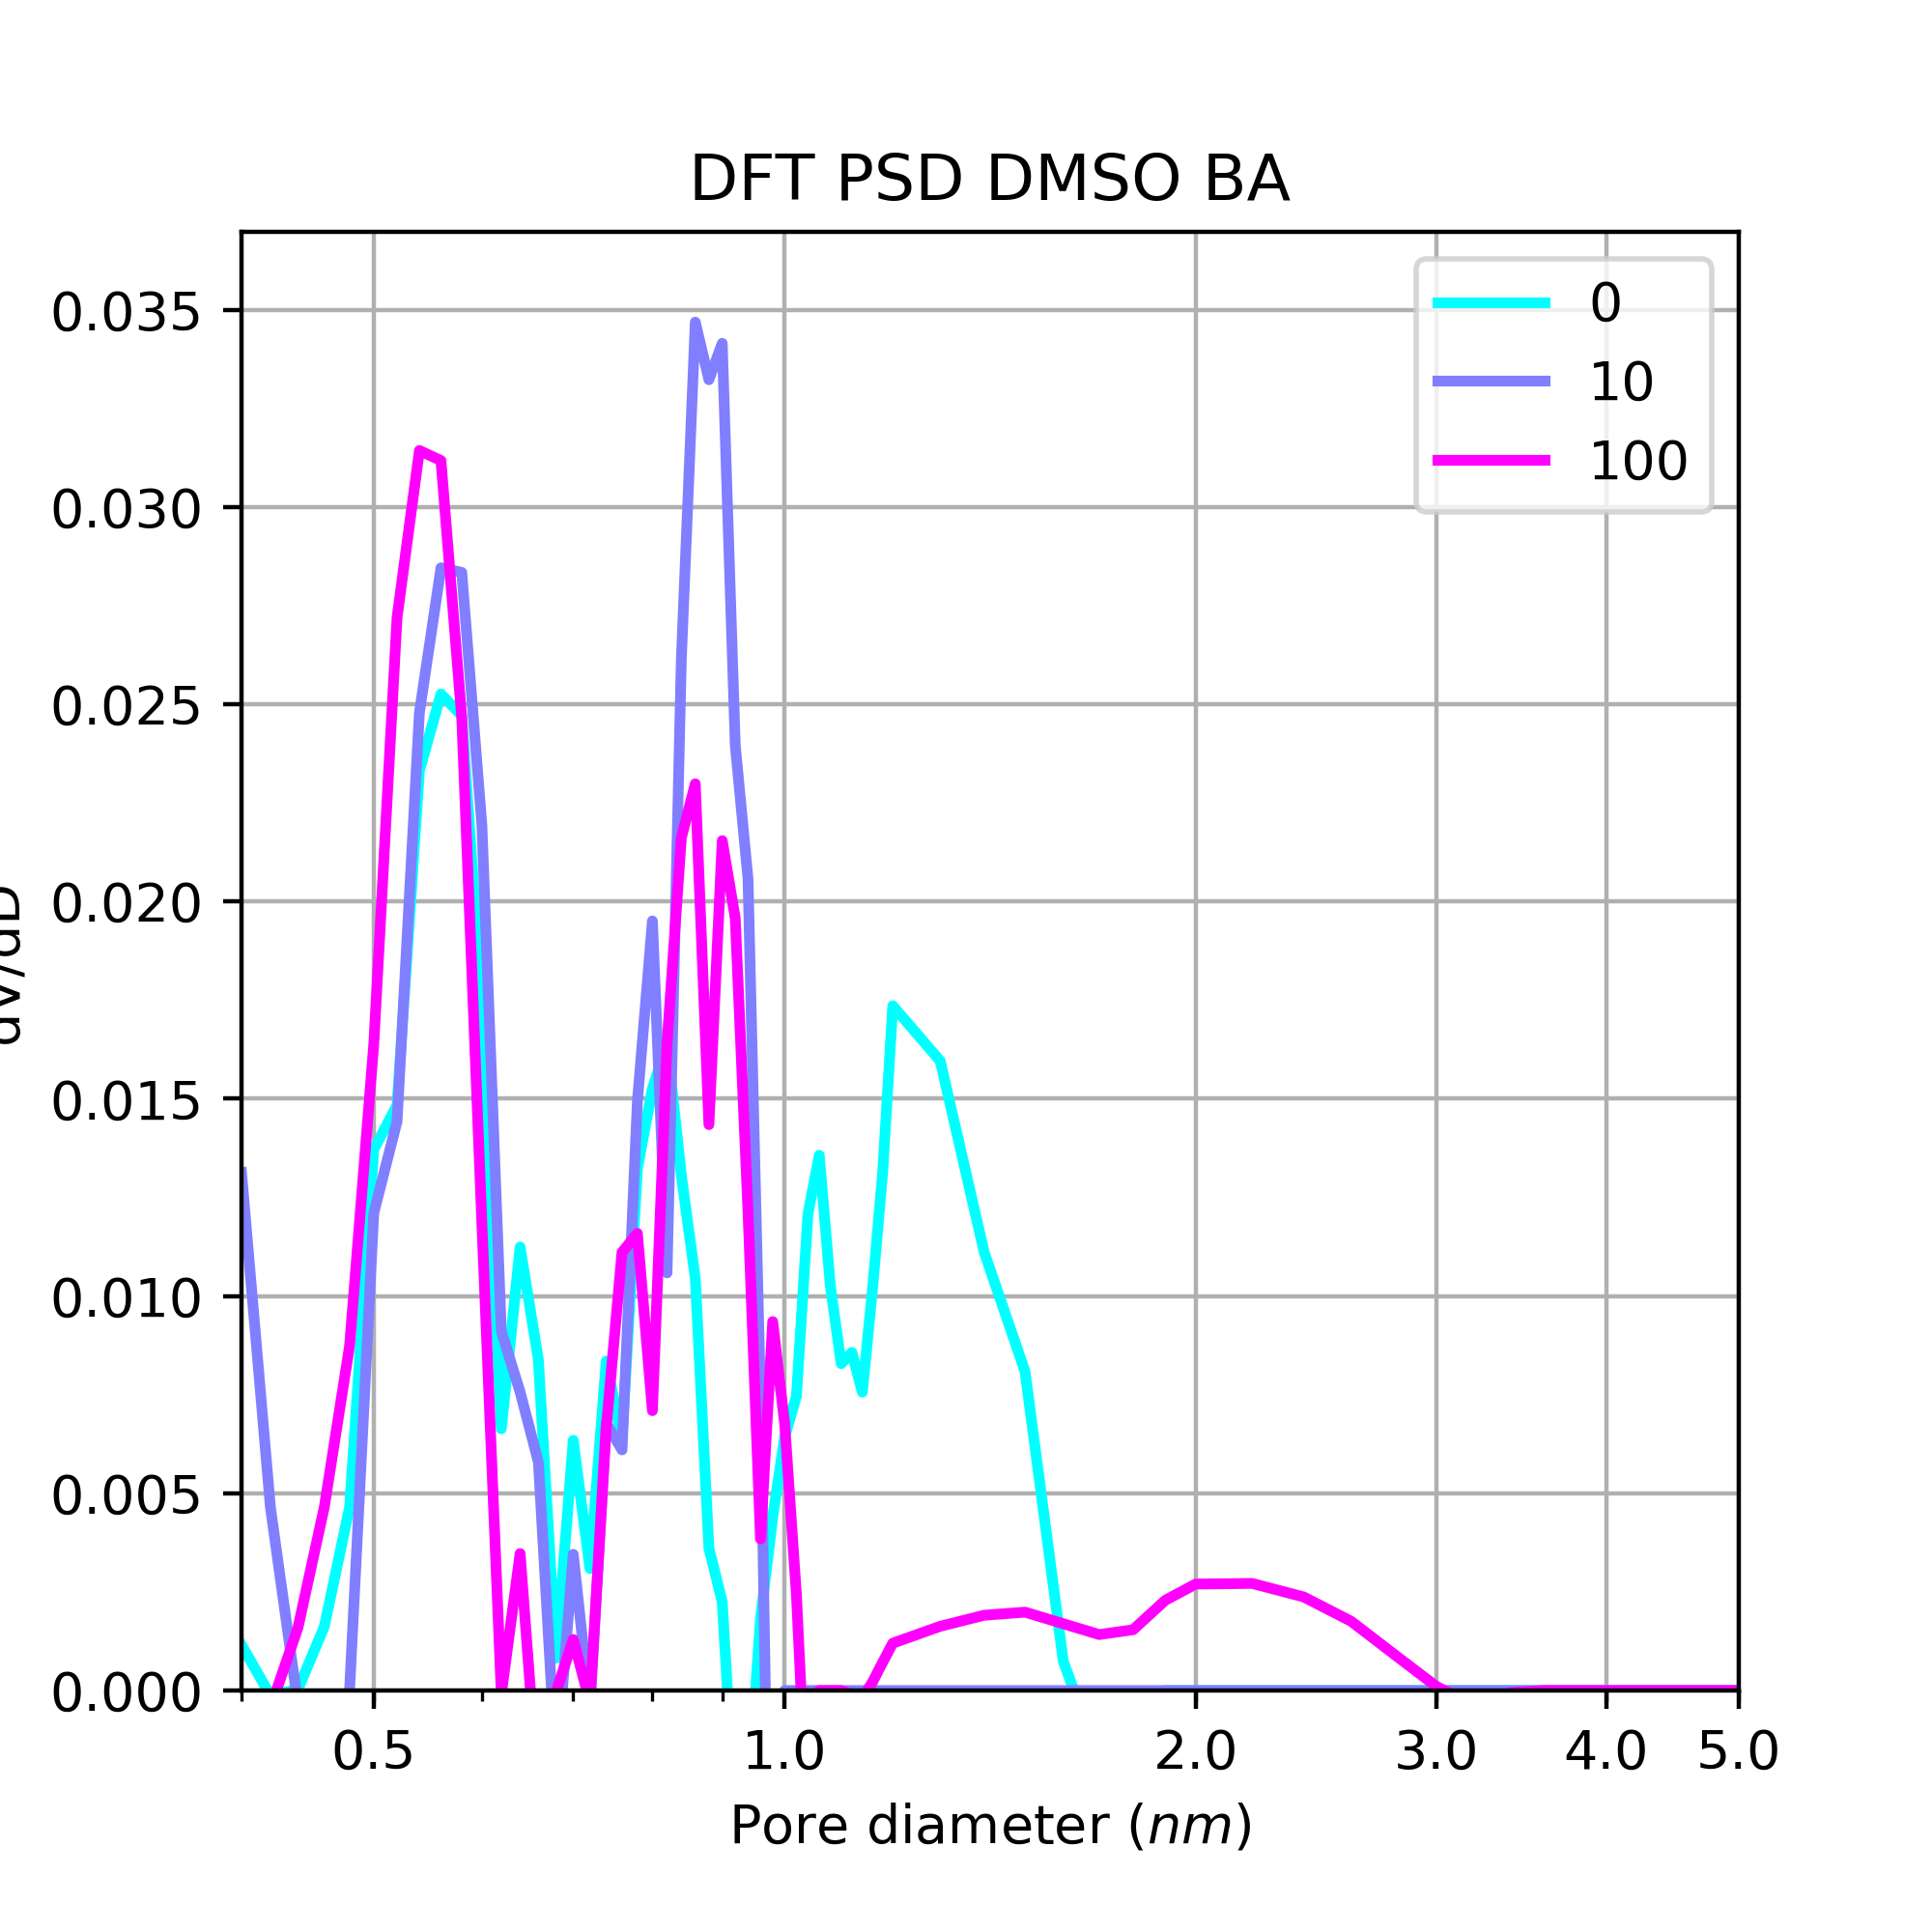
\includegraphics[width=\textwidth]{n2phys/dmso-ba-psd-dft}%
        \label{appx:def:fgr:psd-dmso-ba-dft}
    \end{subfigure}%

\end{figure}
